\documentclass[12pt,a4paper]{article}
\usepackage{booktabs}
\usepackage{multirow}
\usepackage{graphicx}
\usepackage{caption}
\usepackage{subcaption}
\usepackage{longtable}
\usepackage{geometry}
\usepackage{lmodern}
\usepackage[T1]{fontenc}
\usepackage[utf8]{inputenc}
\usepackage{microtype}
\usepackage{float}
\usepackage{rotating}
\usepackage{hyperref}

%% subcaption styling
\captionsetup[subfigure]{labelfont=bf, textfont=normalfont,
                          singlelinecheck=false, justification=raggedright}

\geometry{margin=2.5cm}

\graphicspath{{../figures/}{../maps/}}
\DeclareGraphicsExtensions{.png}

\title{TB in Bangladesh: Data Appendix\\
       \large Supplementary Tables and Figures}
\author{TB Bangladesh Review}
\date{\today}

\begin{document}
\maketitle
\tableofcontents
\clearpage

%% ─── Tables ────────────────────────────────────────────────────────────────
\section{Supplementary Tables}

%% Tables 1A and 1B share the counter value "1"; label suffix set manually.
\renewcommand{\thetable}{1A}
\begin{table}[htbp]
\centering
\caption{Current tuberculosis situation in Bangladesh}
\label{tab:overview}
\small
\begin{tabular}{p{3.2cm}p{4.5cm}p{7.0cm}}
\toprule
\textbf{Category} & \textbf{Key metric / status} & \textbf{Critical impacts \& details} \\
\midrule
Annual Incidence & $\approx$379,000 new cases per year & One of the WHO's 30 highest TB-burden countries. \\[3pt]
Annual Mortality & $\approx$44,000 deaths per year & Averages over 120 fatalities every single day. \\[3pt]
Funding Status & Critical Crisis & Sudden cuts from USAID and the Global Fund have left programmes near collapse. \\[3pt]
Workforce Impact & 1{,}600$+$ health workers laid off & Loss of specialised staff has fractured national preventive operations. \\[3pt]
MDR-TB Burden & $\approx$5{,}000 cases annually & Multidrug-resistant TB is rising; fewer than half of these cases are detected. \\[3pt]
Childhood TB & Critically underdiagnosed & Detection rates for children under five remain dangerously below the 10--15\,\% global benchmark. \\[3pt]
Diagnostic Upgrades & 600$+$ molecular tools deployed & Transitioning away from traditional microscopy to rapid, highly sensitive testing. \\[3pt]
Primary Drivers & Urban density \& climatic factors & Malnutrition, overcrowded cities (Dhaka), and flooding accelerate transmission. \\[3pt]
\bottomrule
\end{tabular}
\par\smallskip
\raggedright\footnotesize Sources: WHO Global TB Report 2024; NTP Bangladesh Annual Report 2023; Global Fund Programme Update 2024; USAID Bangladesh Health Office.
\end{table}
\clearpage

\addtocounter{table}{-1}%   keep counter at 1 for the B sub-table
\renewcommand{\thetable}{1B}
\begin{table}[htbp]
\centering
\caption{Precise tuberculosis infection state and risk profiles --- Bangladesh}
\label{tab:risk_profiles}
\small
\begin{tabular}{p{3.2cm}p{4.5cm}p{7.0cm}}
\toprule
\textbf{Category} & \textbf{Specific indicator / metric} & \textbf{Precise statistical value \& context} \\
\midrule
Global Burden Rank & National Standing & 6th globally in overall tuberculosis disease burden. \\[3pt]
Incidence Rate & Plateaued Transmission & 221 cases per 100{,}000 population; stagnant for 6 consecutive years. \\[3pt]
Annual Mortality & Flatlined Progress & 44{,}000 deaths per year (averaging exactly 121 lives lost daily). \\[3pt]
Notification Gap & Missing / Undetected Cases & $\approx$66{,}000 cases go undetected annually out of 379{,}000 estimated. \\[3pt]
Gender Risk & Male Vulnerability Profile & Men carry an adjusted relative risk (aRR\,$=$\,1.58) for treatment failure. \\[3pt]
Elderly Risk & Age 60$+$ Mortality & Mortality rises to 6.4\,\% (aRR\,$=$\,3.53) vs.\ 1.0\,\% in young adults. \\[3pt]
Pediatric Risk & Under-5 Mortality Rate & Children under five face a 5.4\,\% mortality rate once infected. \\[3pt]
Retreatment Risk & Prior Exposure Failure & Retreatment patients carry a 1.71--1.78$\times$ higher risk of clinical failure. \\[3pt]
\bottomrule
\end{tabular}
\par\smallskip
\raggedright\footnotesize aRR = adjusted relative risk. Sources: WHO Global TB Report 2024; Islam et al.\ (2023); NTP Bangladesh outcome cohort analyses; WHO Global TB Database.
\end{table}
\renewcommand{\thetable}{\arabic{table}}%  restore normal numbering
\clearpage

\begin{sidewaystable}
\centering
\caption{Dataset used for the study --- Bangladesh, 2000--2024}
\label{tab:dataset}
\footnotesize
\begin{tabular}{lrrrrrrrrrrrrrrr}
\toprule
\textbf{Year} & \textbf{Pop} & \textbf{$\rho$} & \textbf{UPop} & \textbf{RPop} & \textbf{GDP} & \textbf{HDI} & \textbf{Pov} & \textbf{PM$_{2.5}$} & \textbf{Temp} & \textbf{Hum} & \textbf{$E_{\mathrm{inc}}$} & \textbf{$E_{\mathrm{mort}}$} & \textbf{Notif} & \textbf{CDR} & \textbf{TSR} \\
 & (M) & (km$^{-2}$) & (M) & (M) & (USD) &  & (\%) & ($\mu$g\,m$^{-3}$) & (\textdegree C) & (\%) & ($\times 10^3$) & ($\times 10^3$) & ($\times 10^3$) & (\%) & (\%) \\
\midrule
2000 & 134.5 & 1,033 & 31.1 & 103.5 & 397 & 0.485 & 41.4 & 53.2 & 25.9 & 73.4 & 298 & 96 & 76 & 25 & 81 \\
2001 & 136.6 & 1,049 & 32.5 & 104.1 & 395 & 0.492 & 39.6 & 53.5 & 25.9 & 73.4 & 303 & 98 & 76 & 25 & 83 \\
2002 & 138.6 & 1,065 & 34.0 & 104.7 & 394 & 0.499 & 37.8 & 54.0 & 25.8 & 73.2 & 307 & 97 & 83 & 27 & 84 \\
2003 & 140.6 & 1,080 & 35.4 & 105.2 & 427 & 0.505 & 35.9 & 54.4 & 25.8 & 73.7 & 312 & 97 & 88 & 28 & 85 \\
2004 & 142.7 & 1,096 & 37.0 & 105.7 & 456 & 0.511 & 34.1 & 54.7 & 25.9 & 72.7 & 316 & 95 & 98 & 31 & 90 \\
2005 & 144.7 & 1,112 & 38.5 & 106.2 & 480 & 0.518 & 32.3 & 54.7 & 26.2 & 72.8 & 320 & 86 & 123 & 38 & 90 \\
2006 & 146.2 & 1,123 & 40.0 & 106.2 & 490 & 0.524 & 30.9 & 53.2 & 26.5 & 71.4 & 324 & 79 & 145 & 45 & 91 \\
2007 & 147.7 & 1,134 & 41.6 & 106.1 & 538 & 0.527 & 29.4 & 50.1 & 25.7 & 73.2 & 327 & 80 & 147 & 45 & 90 \\
2008 & 149.2 & 1,146 & 43.2 & 106.0 & 613 & 0.530 & 28.0 & 46.4 & 25.9 & 73.4 & 331 & 79 & 151 & 46 & 91 \\
2009 & 150.7 & 1,157 & 44.8 & 105.9 & 679 & 0.541 & 26.5 & 43.4 & 26.5 & 70.2 & 334 & 77 & 161 & 48 & 91 \\
2010 & 152.2 & 1,169 & 46.4 & 105.8 & 757 & 0.553 & 25.1 & 56.1 & 26.6 & 70.4 & 337 & 81 & 154 & 46 & 91 \\
2011 & 153.6 & 1,180 & 48.2 & 105.5 & 837 & 0.561 & 24.2 & 54.2 & 25.8 & 70.9 & 340 & 82 & 154 & 45 & 91 \\
2012 & 155.1 & 1,191 & 49.9 & 105.2 & 860 & 0.572 & 23.2 & 56.2 & 26.1 & 70.2 & 343 & 78 & 169 & 49 & 92 \\
2013 & 156.5 & 1,202 & 51.7 & 104.8 & 958 & 0.574 & 22.3 & 57.0 & 26.1 & 70.5 & 346 & 73 & 185 & 53 & 93 \\
2014 & 157.9 & 1,213 & 53.5 & 104.5 & 1,094 & 0.583 & 21.4 & 56.0 & 26.2 & 69.8 & 349 & 72 & 191 & 55 & 93 \\
2015 & 159.4 & 1,224 & 55.3 & 104.1 & 1,224 & 0.602 & 20.4 & 55.4 & 26.2 & 70.8 & 353 & 67 & 207 & 59 & 93 \\
2016 & 160.8 & 1,234 & 57.2 & 103.6 & 1,649 & 0.612 & 19.5 & 57.6 & 26.7 & 72.6 & 356 & 62 & 222 & 62 & 94 \\
2017 & 162.1 & 1,245 & 59.1 & 103.1 & 1,811 & 0.622 & 17.2 & 52.2 & 26.4 & 73.4 & 359 & 56 & 243 & 68 & 94 \\
2018 & 163.5 & 1,256 & 61.0 & 102.6 & 1,965 & 0.635 & 15.0 & 52.9 & 26.1 & 71.6 & 362 & 47 & 267 & 74 & 94 \\
2019 & 164.9 & 1,267 & 62.9 & 102.0 & 2,130 & 0.644 & 12.7 & 46.3 & 26.4 & 72.5 & 365 & 39 & 292 & 80 & 95 \\
2020 & 166.3 & 1,278 & 64.9 & 101.4 & 2,249 & 0.655 & 10.4 & 42.5 & 26.2 & 74.8 & 368 & 44 & 230 & 63 & 95 \\
2021 & 167.8 & 1,289 & 66.8 & 101.0 & 2,483 & 0.661 & 8.2 & 44.6 & 26.8 & 71.9 & 371 & 45 & 307 & 83 & 97 \\
2022 & 169.4 & 1,301 & 68.8 & 100.6 & 2,716 & 0.670 & 5.9 & 41.4 & 27.0 & 73.0 & 375 & 44 & 262 & 70 & 95 \\
2023 & 171.5 & 1,317 & 70.8 & 100.7 & 2,551 & 0.670 & 5.9 & 43.9 & 30.0 & 64.0 & 379 & 44 & 303 & 80 & 96 \\
2024 & 173.6 & 1,333 & 72.9 & 100.7 & 2,593 & 0.670 & 5.9 & 47.6 & 29.4 & 75.0 & 384 & 44 & 314 & 82 & --- \\
\bottomrule
\end{tabular}
\par\smallskip
\raggedright\footnotesize Abbreviations: Pop, total population (millions); $\rho$, population density (per km$^{2}$); UPop, urban population (millions); RPop, rural population (millions); GDP, gross domestic product per capita (current USD); HDI, Human Development Index; Pov, poverty headcount ratio (\% below \$2.15/day --- interpolated in non-survey years); PM$_{2.5}$, national mean ambient PM$_{2.5}$ ($\mu$g\,m$^{-3}$); Temp, mean annual dry-bulb temperature (\textdegree C, BMD Dhaka station); Hum, mean annual relative humidity (\%, BMD Dhaka station); $E_{\mathrm{inc}}$, estimated TB incidence cases ($\times 10^3$); $E_{\mathrm{mort}}$, estimated TB deaths ($\times 10^3$, HIV-negative); Notif, notified new and relapse TB cases ($\times 10^3$); CDR, case detection rate (\%); TSR, treatment success rate (\%). Sources: Worldometer (population); World Bank Open Data (GDP, poverty); UNDP (HDI); World Bank\,/\,WHO\,/\,CAMS (PM$_{2.5}$); BMD via DENV-Data-Analysis (temperature, humidity); WHO Global TB Programme (TB estimates, notifications, outcomes).
\end{sidewaystable}
\clearpage

\begin{table}[htbp]
\centering
\caption{Summary of descriptive statistics for study variables --- Bangladesh, 2000--2024}
\label{tab:descriptive_stats}
\small
\begin{tabular}{lrrrr}
\toprule
\textbf{Variable} & \textbf{Mean} & \textbf{Standard deviation} & \textbf{Min} & \textbf{Max} \\
\midrule
Population (M) & 154.65 & 11.33 & 134.54 & 173.56 \\
Density (per km$^{2}$) & 1188 & 87 & 1033 & 1333 \\
Urban population (M) & 50.69 & 12.85 & 31.05 & 72.90 \\
Rural population (M) & 103.96 & 1.94 & 100.61 & 106.22 \\
GDP per capita (USD) & 1,230 & 829 & 394 & 2,716 \\
Human Development Index & 0.577 & 0.063 & 0.485 & 0.670 \\
Poverty rate (\%) & 22.93 & 10.87 & 5.90 & 41.40 \\
PM$_{2.5}$ ($\mu$g\,m$^{-3}$) & 51.26 & 5.10 & 41.40 & 57.60 \\
Mean temperature (\textdegree C) & 26.48 & 1.03 & 25.71 & 30.00 \\
Humidity (\%) & 71.96 & 2.20 & 64.00 & 75.00 \\
Estimated incidence ($\times 10^3$) & 342.36 & 24.87 & 298.00 & 384.00 \\
Estimated deaths ($\times 10^3$) & 70.48 & 19.93 & 39.00 & 98.00 \\
Notified cases ($\times 10^3$) & 185.93 & 75.93 & 75.56 & 314.18 \\
CDR (\%) & 53.08 & 18.58 & 25.00 & 83.00 \\
TSR (\%) & 91.21 & 4.17 & 81.00 & 97.00 \\
\bottomrule
\end{tabular}
\par\smallskip
\raggedright\footnotesize Statistics computed over all available annual observations, 2000--2024 ($n = 25$ for most variables; TSR reported with $\approx$2-year lag and missing for the most recent cohort years). CDR = case detection rate; TSR = treatment success rate. Poverty rate interpolated linearly between World Bank HIES survey anchors (2000, 2005, 2010, 2016, 2022); 2023--2024 held at 2022 value. See Table~2 for the full annual series.
\end{table}
\clearpage

\begin{table}[htbp]
\centering
\caption{WHO TB Burden Estimates — Bangladesh, 2000--2024}
\label{tab:burden}
\small
\begin{tabular}{lrrrrrrr}
\toprule
\multicolumn{1}{c}{\textbf{Year}} &\multicolumn{3}{c}{\textbf{Incidence rate (per 100\,k)}} &\multicolumn{3}{c}{\textbf{Mortality rate (per 100\,k)}} &\multicolumn{1}{c}{\textbf{CDR (\%)}} \\
\cmidrule(lr){2-4} \cmidrule(lr){5-7}
& Estimate & Low & High & Estimate & Low & High & \\
\midrule
2000 & 221 & 161 & 291 & 71.0 & 45.0 & 103.0 & 25 \\
2001 & 221 & 161 & 291 & 72.0 & 46.0 & 104.0 & 25 \\
2002 & 221 & 161 & 291 & 70.0 & 44.0 & 101.0 & 27 \\
2003 & 221 & 161 & 291 & 69.0 & 44.0 & 100.0 & 28 \\
2004 & 221 & 161 & 291 & 66.0 & 42.0 & 96.0 & 31 \\
2005 & 221 & 161 & 291 & 60.0 & 38.0 & 86.0 & 38 \\
2006 & 221 & 161 & 291 & 54.0 & 35.0 & 77.0 & 45 \\
2007 & 221 & 161 & 291 & 54.0 & 35.0 & 77.0 & 45 \\
2008 & 221 & 161 & 291 & 53.0 & 34.0 & 76.0 & 46 \\
2009 & 221 & 161 & 291 & 51.0 & 33.0 & 73.0 & 48 \\
2010 & 221 & 161 & 291 & 53.0 & 34.0 & 77.0 & 46 \\
2011 & 221 & 161 & 291 & 54.0 & 35.0 & 77.0 & 45 \\
2012 & 221 & 161 & 291 & 51.0 & 33.0 & 72.0 & 49 \\
2013 & 221 & 161 & 291 & 47.0 & 30.0 & 67.0 & 53 \\
2014 & 221 & 161 & 291 & 46.0 & 30.0 & 65.0 & 55 \\
2015 & 221 & 161 & 291 & 42.0 & 27.0 & 60.0 & 59 \\
2016 & 221 & 161 & 291 & 39.0 & 25.0 & 56.0 & 62 \\
2017 & 221 & 161 & 291 & 34.0 & 22.0 & 49.0 & 68 \\
2018 & 221 & 161 & 291 & 29.0 & 19.0 & 42.0 & 74 \\
2019 & 221 & 161 & 291 & 24.0 & 15.0 & 35.0 & 80 \\
2020 & 221 & 161 & 291 & 26.0 & 17.0 & 38.0 & 63 \\
2021 & 221 & 161 & 291 & 27.0 & 17.0 & 39.0 & 83 \\
2022 & 221 & 161 & 291 & 26.0 & 17.0 & 38.0 & 70 \\
2023 & 221 & 161 & 291 & 26.0 & 17.0 & 38.0 & 80 \\
2024 & 221 & 161 & 291 & 25.0 & 16.0 & 38.0 & 82 \\
\bottomrule
\end{tabular}
\par\smallskip
\raggedright\footnotesize CDR = case detection rate (notified/estimated $\times$ 100). 95\% confidence intervals from WHO Global TB Programme burden estimates.
\end{table}
\clearpage

\begin{table}[htbp]
\centering
\caption{TB Case Notifications and Programme Performance — Bangladesh, 2000--2024}
\label{tab:notifications}
\small
\resizebox{\textwidth}{!}{
\begin{tabular}{lrrrrrr}
\toprule
\textbf{Year} & \textbf{Total notified} & \textbf{Smear-pos} & \textbf{Extra-pulm} & \textbf{Conf.\ RR/MDR} & \textbf{CDR (\%)} & \textbf{TSR (\%)} \\
\midrule
2000 & 75,557 & 38,484 & 5,914 & --- & 25 & 81 \\
2001 & 76,302 & 40,777 & 5,778 & --- & 25 & 83 \\
2002 & 83,485 & 46,811 & 6,351 & --- & 27 & 84 \\
2003 & 88,156 & 53,618 & 7,120 & --- & 28 & 85 \\
2004 & 98,336 & 62,694 & 8,626 & --- & 31 & 90 \\
2005 & 123,118 & 84,848 & 11,318 & --- & 38 & 90 \\
2006 & 145,186 & 101,967 & 14,436 & --- & 45 & 91 \\
2007 & 147,342 & 104,296 & 16,106 & --- & 45 & 90 \\
2008 & 151,062 & 106,373 & 18,359 & --- & 46 & 91 \\
2009 & 160,875 & 109,402 & 21,999 & --- & 48 & 91 \\
2010 & 153,892 & 105,772 & 23,506 & --- & 46 & 91 \\
2011 & 154,358 & 98,948 & 27,329 & --- & 45 & 91 \\
2012 & 168,683 & 106,790 & 30,549 & --- & 49 & 92 \\
2013 & 184,506 & --- & 33,704 & --- & 53 & 93 \\
2014 & 191,166 & --- & 37,406 & 994 & 55 & 93 \\
2015 & 206,915 & --- & 42,000 & 954 & 59 & 93 \\
2016 & 222,248 & --- & 43,549 & 969 & 62 & 94 \\
2017 & 242,639 & --- & 44,745 & 944 & 68 & 94 \\
2018 & 267,143 & --- & 49,775 & 1,228 & 74 & 94 \\
2019 & 291,595 & --- & 53,275 & 1,373 & 80 & 95 \\
2020 & 230,081 & --- & 42,244 & --- & 63 & 95 \\
2021 & 306,701 & --- & 55,994 & --- & 83 & 97 \\
2022 & 261,957 & --- & 62,692 & --- & 70 & 95 \\
2023 & 302,813 & --- & 66,370 & --- & 80 & 96 \\
2024 & 314,180 & --- & 67,584 & --- & 82 & --- \\
\bottomrule
\end{tabular}
}
\par\smallskip
\raggedright\footnotesize Smear-pos = new smear-positive pulmonary TB; reporting shifted to GeneXpert-based definitions after 2011. Extra-pulm = extra-pulmonary TB. CDR = case detection rate; TSR = treatment success rate (\%). Source: WHO Global TB Programme notifications and outcomes datasets.
\end{table}
\clearpage

\begin{table}[htbp]
\centering
\caption{TB Treatment Outcomes — Bangladesh (cohort years)}
\label{tab:outcomes}
\small
\begin{tabular}{lrrrrrr}
\toprule
\textbf{Year} & \textbf{Cohort} & \textbf{Success} & \textbf{TSR (\%)} & \textbf{Died} & \textbf{Failed} & \textbf{Lost} \\
\midrule
1994 & 1,635 & 1,121 & 73 & 96 & 32 & 180 \\
1995 & 10,867 & 7,218 & 71 & 530 & 166 & 1,094 \\
1996 & 29,674 & 17,150 & 63 & 1,008 & 416 & 4,890 \\
1997 & 33,784 & 22,391 & 73 & 1,299 & 413 & 5,402 \\
1998 & 38,029 & 27,668 & 77 & 1,717 & 318 & 4,294 \\
1999 & 37,821 & 28,143 & 79 & 1,572 & 277 & 3,588 \\
2000 & 38,484 & 29,655 & 81 & 1,578 & 300 & 3,355 \\
2001 & 40,771 & 32,294 & 83 & 1,760 & 330 & 3,088 \\
2002 & 46,811 & 37,953 & 84 & 2,215 & 325 & 3,268 \\
2003 & 53,618 & 44,581 & 85 & 2,574 & 341 & 2,840 \\
2004 & 62,694 & 55,468 & 90 & 2,400 & 439 & 1,745 \\
2005 & 84,848 & 76,833 & 90 & 2,986 & 541 & 1,745 \\
2006 & 101,761 & 92,921 & 91 & 3,294 & 555 & 1,993 \\
2007 & 104,296 & 94,778 & 90 & 3,468 & 583 & 1,796 \\
2008 & 106,089 & 95,316 & 91 & 3,860 & 781 & 1,903 \\
2009 & 109,075 & 98,943 & 91 & 4,034 & 915 & 1,906 \\
2010 & 105,659 & 95,565 & 91 & 4,061 & 876 & 1,853 \\
2011 & 98,932 & 89,989 & 91 & 3,737 & 808 & 1,641 \\
2012 & 164,587 & 151,447 & 92 & 6,681 & 933 & 2,622 \\
2013 & 184,077 & 170,893 & 93 & 7,395 & 822 & 2,251 \\
2014 & 191,141 & 177,715 & 93 & 7,252 & 1,027 & 2,232 \\
2015 & 206,907 & 192,571 & 93 & 7,806 & 1,148 & 2,084 \\
2016 & 222,252 & 207,832 & 94 & 8,040 & 1,187 & 1,640 \\
2017 & 242,640 & 227,305 & 94 & 8,762 & 1,030 & 1,773 \\
2018 & 267,143 & 252,170 & 94 & 8,363 & 876 & 1,707 \\
2019 & 289,863 & 274,452 & 95 & 8,431 & 905 & 1,753 \\
2020 & 228,779 & 218,114 & 95 & 6,482 & 693 & 838 \\
2021 & 306,860 & 296,487 & 97 & 5,862 & 684 & 819 \\
2022 & 262,044 & 249,315 & 95 & 6,790 & 782 & 1,197 \\
2023 & 301,256 & 287,717 & 96 & 7,563 & 680 & 1,577 \\
2024 & \multicolumn{6}{c}{\textit{Not yet reported by WHO}} \\
\bottomrule
\end{tabular}
\par\smallskip
\raggedright\footnotesize Outcomes reported with $\approx$2-year lag (cohort year shown). Pre-2012: smear-positive cohort used as proxy for total cohort. TSR = treated successfully / cohort $\times$ 100. 2024 data pending WHO Global TB Report 2026. Source: WHO Global TB Programme outcomes dataset.
\end{table}
\clearpage

\begin{table}[htbp]
\centering
\caption{Cumulative TB Burden by Division --- Bangladesh, 2000--2024. Split at 2015 to reflect the creation of Mymensingh division.}
\label{tab:division_cumulative}
\small
\begin{tabular}{lrrrr}
\toprule
\textbf{Division} & \textbf{Cases 2000--14} & \textbf{Cases 2015--24} & \textbf{Total 2000--24} & \textbf{Est.\ deaths} \\
\midrule
Dhaka$^{\dagger}$ & 306,000 & 171,900 & 477,900 & 159,541 \\
Chattogram & 147,000 & 76,600 & 223,600 & 74,646 \\
Rajshahi & 121,500 & 59,600 & 181,100 & 60,458 \\
Rangpur & 112,500 & 53,600 & 166,100 & 55,451 \\
Khulna & 96,000 & 42,600 & 138,600 & 46,270 \\
Sylhet & 93,000 & 40,600 & 133,600 & 44,601 \\
Mymensingh$^{\ddagger}$ & --- & 53,600 & 53,600 & 17,894 \\
Barishal & 51,000 & 23,300 & 74,300 & 24,804 \\
\midrule
\textbf{Bangladesh total} & \textbf{927,000} & \textbf{521,800} & \textbf{1,448,800} & \textbf{483,665} \\
\bottomrule
\end{tabular}
\par\smallskip
\raggedright\footnotesize Estimated deaths = total cases $\times$ national CFR (case-fatality ratio $\approx$\,33.4\,\%, derived from WHO burden estimates). $^{\dagger}$Dhaka 2000--2014 includes the territory that became Mymensingh division in 2015; the two cannot be separated from published records. $^{\ddagger}$Mymensingh established as a separate division in 2015; pre-2015 burden is subsumed within the Dhaka 2000--2014 figure. Case counts derived from NTP Bangladesh / DGHS Annual Reports.
\end{table}
\clearpage

\begin{table}[htbp]
\centering
\caption{Socioeconomic Indicators --- Bangladesh, 2000--2024}
\label{tab:socioeconomic}
\small
\resizebox{\textwidth}{!}{
\begin{tabular}{lrrrrrrrr}
\toprule
\textbf{Year} & \textbf{GDP p.c.\ (USD)} & \textbf{HDI} & \textbf{Poverty (\%)} & \textbf{Urban pop.\ (M)} & \textbf{Rural pop.\ (M)} & \textbf{Density (km$^{-2}$)} & \textbf{Health exp.\ (USD)} & \textbf{BCG (\%)} \\
\midrule
2000 & 397 & 0.485 & 41.4 & 31.1 & 103.5 & 1,033 & 8 & 94 \\
2001 & 395 & 0.492 & 39.6$^\dagger$ & 32.5 & 104.1 & 1,049 & 8 & 95 \\
2002 & 394 & 0.499 & 37.8$^\dagger$ & 34.0 & 104.7 & 1,065 & 9 & 95 \\
2003 & 427 & 0.505 & 35.9$^\dagger$ & 35.4 & 105.2 & 1,080 & 10 & 93 \\
2004 & 456 & 0.511 & 34.1$^\dagger$ & 37.0 & 105.7 & 1,096 & 11 & 96 \\
2005 & 480 & 0.518 & 32.3 & 38.5 & 106.2 & 1,112 & 11 & 97 \\
2006 & 490 & 0.524 & 30.9$^\dagger$ & 40.0 & 106.2 & 1,123 & 12 & 97 \\
2007 & 538 & 0.527 & 29.4$^\dagger$ & 41.6 & 106.1 & 1,134 & 14 & 98 \\
2008 & 613 & 0.530 & 28.0$^\dagger$ & 43.2 & 106.0 & 1,146 & 16 & 99 \\
2009 & 679 & 0.541 & 26.5$^\dagger$ & 44.8 & 105.9 & 1,157 & 18 & 99 \\
2010 & 757 & 0.553 & 25.1 & 46.4 & 105.8 & 1,169 & 21 & 98 \\
2011 & 837 & 0.561 & 24.2$^\dagger$ & 48.2 & 105.5 & 1,180 & 23 & 99 \\
2012 & 860 & 0.572 & 23.2$^\dagger$ & 49.9 & 105.2 & 1,191 & 23 & 98 \\
2013 & 958 & 0.574 & 22.3$^\dagger$ & 51.7 & 104.8 & 1,202 & 27 & 99 \\
2014 & 1,094 & 0.583 & 21.4$^\dagger$ & 53.5 & 104.5 & 1,213 & 30 & 99 \\
2015 & 1,224 & 0.602 & 20.4$^\dagger$ & 55.3 & 104.1 & 1,224 & 33 & 99 \\
2016 & 1,649 & 0.612 & 19.5 & 57.2 & 103.6 & 1,234 & 39 & 99 \\
2017 & 1,811 & 0.622 & 17.2$^\dagger$ & 59.1 & 103.1 & 1,245 & 42 & 99 \\
2018 & 1,965 & 0.635 & 15.0$^\dagger$ & 61.0 & 102.6 & 1,256 & 45 & 99 \\
2019 & 2,130 & 0.644 & 12.7$^\dagger$ & 62.9 & 102.0 & 1,267 & 45 & 99 \\
2020 & 2,249 & 0.655 & 10.4$^\dagger$ & 64.9 & 101.4 & 1,278 & 49 & 99 \\
2021 & 2,483 & 0.661 & 8.2$^\dagger$ & 66.8 & 101.0 & 1,289 & 56 & 99 \\
2022 & 2,716 & 0.670 & 5.9 & 68.8 & 100.6 & 1,301 & 57 & 99 \\
2023 & 2,551 & 0.670 & 5.9$^\dagger$ & 70.8 & 100.7 & 1,317 & 53 & 99 \\
2024 & 2,593 & 0.670 & 5.9$^\dagger$ & 72.9 & 100.7 & 1,333 & --- & 99 \\
\bottomrule
\end{tabular}
}
\par\smallskip
\raggedright\footnotesize GDP p.c.\ = gross domestic product per capita (current USD; World Bank). HDI = Human Development Index (UNDP). Poverty = population below \$2.15/day international poverty line (\%; World Bank SI.POV.DDAY); survey years 2000, 2005, 2010, 2016, 2022; $\dagger$~linearly interpolated between survey anchors; 2023--2024 held at 2022 value. Urban and Rural pop.\ in millions; Density per km$^2$: Worldometer Bangladesh (via DENV-Data-Analysis, github.com/awnonbhowmik/DENV-Data-Analysis); 2000 estimated. Health exp.\ = current health expenditure per capita (USD; World Bank). BCG = BCG immunisation coverage (\% of infants; World Bank).
\end{table}
\clearpage

\begin{table}[htbp]
\centering
\caption{Environmental Factors --- Bangladesh, 2000--2024}
\label{tab:environmental}
\small
\begin{tabular}{lrrr}
\toprule
\textbf{Year} & \textbf{Mean temp.\ (\textdegree C)} & \textbf{Humidity (\%)} & \textbf{PM\textsubscript{2.5} --- national mean ($\mu$g\,m$^{-3}$)} \\
\midrule
2000 & 25.9 & 73.4 & 53.2 \\
2001 & 25.9 & 73.4 & 53.5 \\
2002 & 25.8 & 73.2 & 54.0 \\
2003 & 25.8 & 73.7 & 54.4 \\
2004 & 25.9 & 72.7 & 54.7 \\
2005 & 26.2 & 72.8 & 54.7 \\
2006 & 26.5 & 71.4 & 53.2 \\
2007 & 25.7 & 73.2 & 50.1 \\
2008 & 25.9 & 73.4 & 46.4 \\
2009 & 26.5 & 70.2 & 43.4 \\
2010 & 26.6 & 70.4 & 56.1 \\
2011 & 25.8 & 70.9 & 54.2 \\
2012 & 26.1 & 70.2 & 56.2 \\
2013 & 26.1 & 70.5 & 57.0 \\
2014 & 26.2 & 69.8 & 56.0 \\
2015 & 26.2 & 70.8 & 55.4 \\
2016 & 26.7 & 72.6 & 57.6 \\
2017 & 26.4 & 73.4 & 52.2 \\
2018 & 26.1 & 71.6 & 52.9 \\
2019 & 26.4 & 72.5 & 46.3 \\
2020 & 26.2 & 74.8 & 42.5 \\
2021 & 26.8 & 71.9 & 44.6 \\
2022 & 27.0 & 73.0 & 41.4 \\
2023 & 30.0 & 64.0 & 43.9 \\
2024 & 29.4 & 75.0 & 47.6 \\
\bottomrule
\end{tabular}
\par\smallskip
\raggedright\footnotesize Temperature and Humidity: Bangladesh Meteorological Department (BMD) Dhaka station annual records (Dry Bulb Temperature, Relative Humidity); sourced from DENV-Data-Analysis (github.com/awnonbhowmik/DENV-Data-Analysis). 2000 values are estimated from adjacent years. PM\textsubscript{2.5} 2000--2020: World Bank indicator EN.ATM.PM25.MC.M3 (national population-weighted). PM\textsubscript{2.5} 2021--2023: WHO GHO indicator SDGPM25 (national total). PM\textsubscript{2.5} 2024: CAMS reanalysis via Open-Meteo. WHO PM\textsubscript{2.5} guideline revised from 10 to 5\,\textmu{}g\,m\textsuperscript{$-3$} in 2021.
\end{table}
\clearpage

\begin{table}[htbp]
\centering
\caption{TB Incidence Rate (per 100,000) and Absolute Cases by Division --- Bangladesh, Selected Years}
\label{tab:division_incidence}
\small
\resizebox{\textwidth}{!}{
\begin{tabular}{lrrrrrrrrrrrr}
\toprule
\multirow{2}{*}{\textbf{Division}} & \multicolumn{2}{c}{\textbf{2000}} & \multicolumn{2}{c}{\textbf{2005}} & \multicolumn{2}{c}{\textbf{2010}} & \multicolumn{2}{c}{\textbf{2015}} & \multicolumn{2}{c}{\textbf{2020}} & \multicolumn{2}{c}{\textbf{2024}} \\
\cmidrule(lr){2-3}\cmidrule(lr){4-5}\cmidrule(lr){6-7}\cmidrule(lr){8-9}\cmidrule(lr){10-11}\cmidrule(lr){12-13}
 & \footnotesize Rate & \footnotesize Cases & \footnotesize Rate & \footnotesize Cases & \footnotesize Rate & \footnotesize Cases & \footnotesize Rate & \footnotesize Cases & \footnotesize Rate & \footnotesize Cases & \footnotesize Rate & \footnotesize Cases \\
\midrule
Barishal & 45 & 4,100 & 40 & 3,600 & 35 & 3,100 & 30 & 2,600 & 25 & 2,100 & 27 & 2,300 \\
Chattogram & 62 & 11,200 & 57 & 10,200 & 52 & 9,200 & 47 & 8,200 & 42 & 7,200 & 44 & 7,600 \\
Dhaka & 85 & 22,500 & 80 & 21,000 & 75 & 19,500 & 70 & 18,000 & 65 & 16,500 & 67 & 17,100 \\
Khulna & 50 & 7,800 & 45 & 6,800 & 40 & 5,800 & 35 & 4,800 & 30 & 3,800 & 32 & 4,200 \\
Mymensingh & --- & --- & --- & --- & --- & --- & 55 & 5,900 & 50 & 4,900 & 52 & 5,300 \\
Rajshahi & 48 & 9,500 & 43 & 8,500 & 38 & 7,500 & 33 & 6,500 & 28 & 5,500 & 30 & 5,900 \\
Rangpur & 52 & 8,900 & 47 & 7,900 & 42 & 6,900 & 37 & 5,900 & 32 & 4,900 & 34 & 5,300 \\
Sylhet & 58 & 7,600 & 53 & 6,600 & 48 & 5,600 & 43 & 4,600 & 38 & 3,600 & 40 & 4,000 \\
\bottomrule
\end{tabular}
}
\par\smallskip
\raggedright\footnotesize Rate = TB incidence rate per 100,000 population. Cases = estimated absolute notified cases. Mymensingh became a separate division in 2015 (shown as --- before that year). Source: NTP Bangladesh / DGHS Annual Reports.
\end{table}
\clearpage

\begin{table}[htbp]
\centering
\caption{TB-Associated Risk Factors --- Bangladesh, 2000--2024}
\label{tab:riskfactors}
\small
\resizebox{\textwidth}{!}{
\begin{tabular}{lrrrr}
\toprule
\textbf{Year} & \textbf{Undernourishment (\%)} & \textbf{Child Stunting (\%$^\dagger$)} & \textbf{Smoking (\%$^\ddagger$)} & \textbf{Health Exp.\ (\% GDP)} \\
\midrule
2000 & --- & 51.1 & 58.1 & 1.81 \\
2001 & 15.5 & 53.2 & --- & 1.77 \\
2002 & 14.6 & 51.4 & --- & 1.93 \\
2003 & 14.8 & 47.8 & --- & 1.96 \\
2004 & 14.7 & 50.5 & --- & 2.00 \\
2005 & 15.1 & 46.2 & 50.7 & 2.06 \\
2006 & 15.4 & 45.1 & --- & 2.11 \\
2007 & 16.1 & 43.2 & 48.0 & 2.17 \\
2008 & 16.9 & --- & --- & 2.12 \\
2009 & 17.9 & --- & --- & 2.18 \\
2010 & 18.2 & --- & 44.2 & 2.29 \\
2011 & 18.0 & 41.3 & --- & 2.36 \\
2012 & 17.3 & 37.0 & --- & 2.35 \\
2013 & 16.7 & 42.0 & --- & 2.30 \\
2014 & 15.6 & 36.2 & --- & 2.28 \\
2015 & 15.2 & 35.0 & 38.9 & 2.27 \\
2016 & 14.4 & --- & --- & 2.39 \\
2017 & 13.4 & --- & --- & 2.37 \\
2018 & 12.0 & 30.9 & --- & 2.32 \\
2019 & 10.9 & 28.0 & --- & 2.13 \\
2020 & 10.8 & --- & 34.4 & 2.18 \\
2021 & 10.3 & --- & 33.8 & 2.27 \\
2022 & 10.6 & 23.6 & 32.9 & 2.22 \\
2023 & 10.4 & --- & --- & 2.17 \\
2024 & --- & --- & --- & --- \\
\bottomrule
\end{tabular}
}
\par\smallskip
\raggedright\footnotesize Undernourishment: FAO prevalence of undernourishment, \% of population (World Bank SN.ITK.DEFC.ZS); annual 2001--2023. $\dagger$~Child stunting: prevalence of stunting, height-for-age, \% of children under-5 (World Bank SH.STA.STNT.ZS); survey years only, shown as --- otherwise. $\ddagger$~Smoking: age-standardised prevalence of current tobacco smoking, \% adults $\geq$15 (World Bank SH.PRV.SMOK); survey years only. Health exp.\ = current health expenditure as \% of GDP (World Bank SH.XPD.CHEX.GD.ZS).
\end{table}
\clearpage

%% ─── Figures ───────────────────────────────────────────────────────────────
\section{Supplementary Figures}
\noindent\textit{Figures are ordered to match the narrative flow of the review:
national burden $\to$ programme performance $\to$ demographics $\to$
geographic distribution $\to$ determinants $\to$ statistical analysis.
Multi-panel figures use lettered sub-panels (A, B, C\ldots).}
\bigskip

%% Figure 1 ─────────────────────────────────────────────────────────────────
\begin{figure}[htbp]
  \centering
  %% Panel A — full width on top
  \begin{subfigure}[t]{\textwidth}
    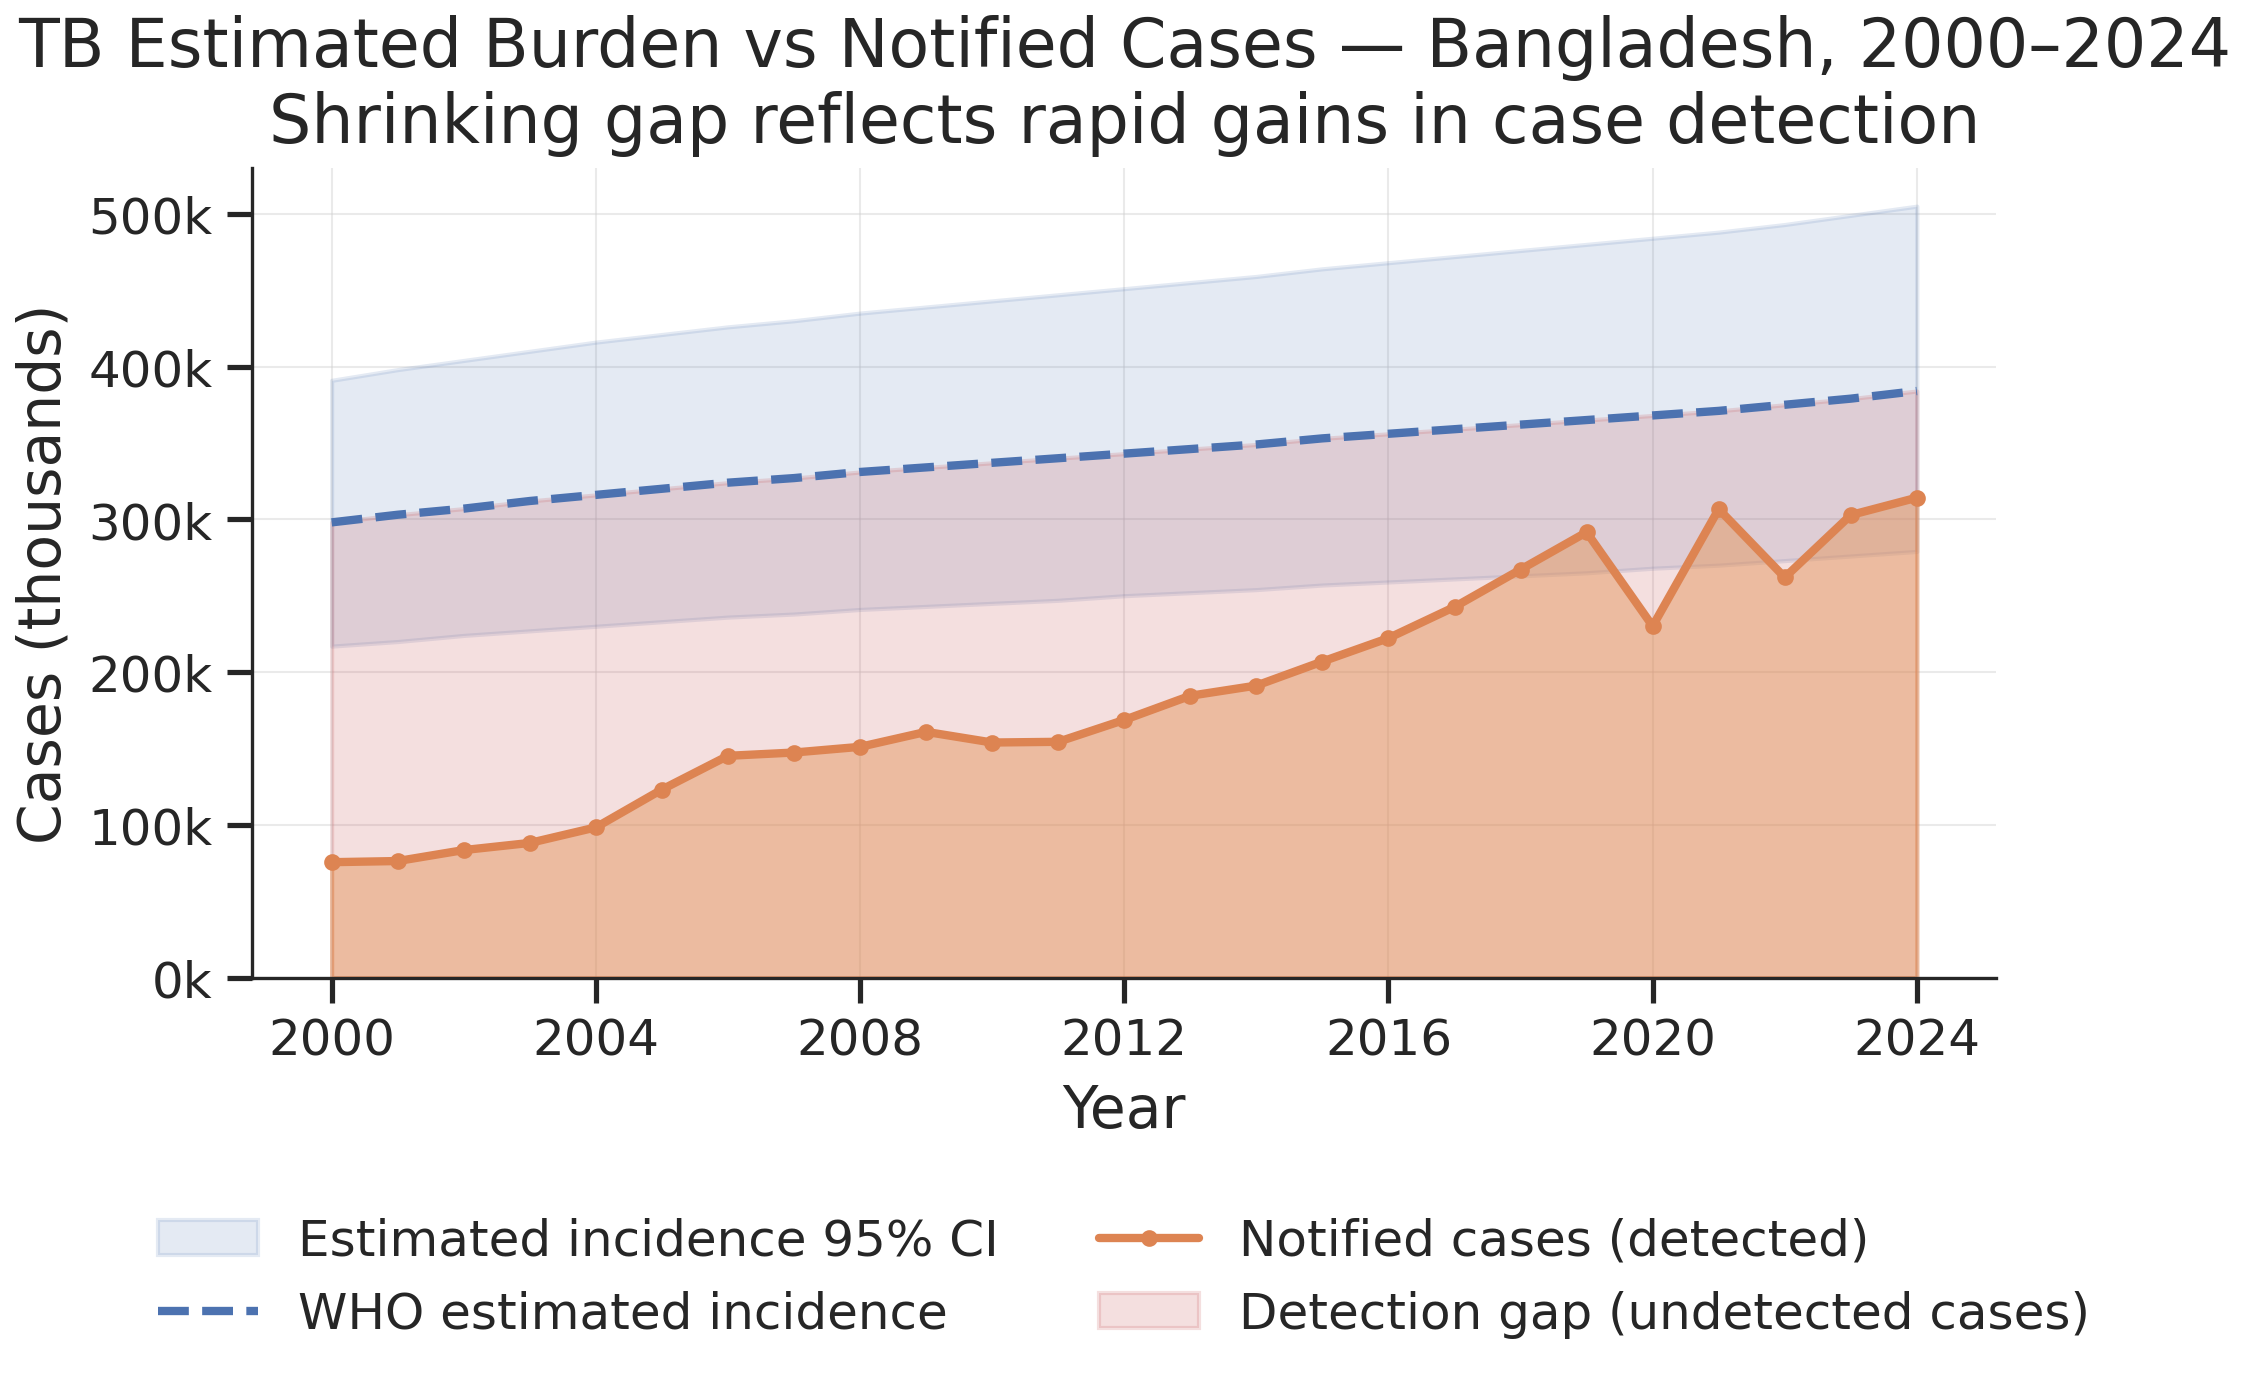
\includegraphics[width=\textwidth]{fig1_incidence_trend}
    \subcaption{Estimated TB burden versus notified cases, 2000--2024.
      The shaded blue band is the WHO 95\,\% confidence interval for estimated incidence;
      the orange filled area represents the detection gap (undetected cases).
      The rapid convergence after 2010 reflects scaled-up DOTS and GeneXpert deployment.}
    \label{fig:1a}
  \end{subfigure}
  \vspace{0.8em}
  %% Panels B and C — side by side
  \begin{subfigure}[t]{0.48\textwidth}
    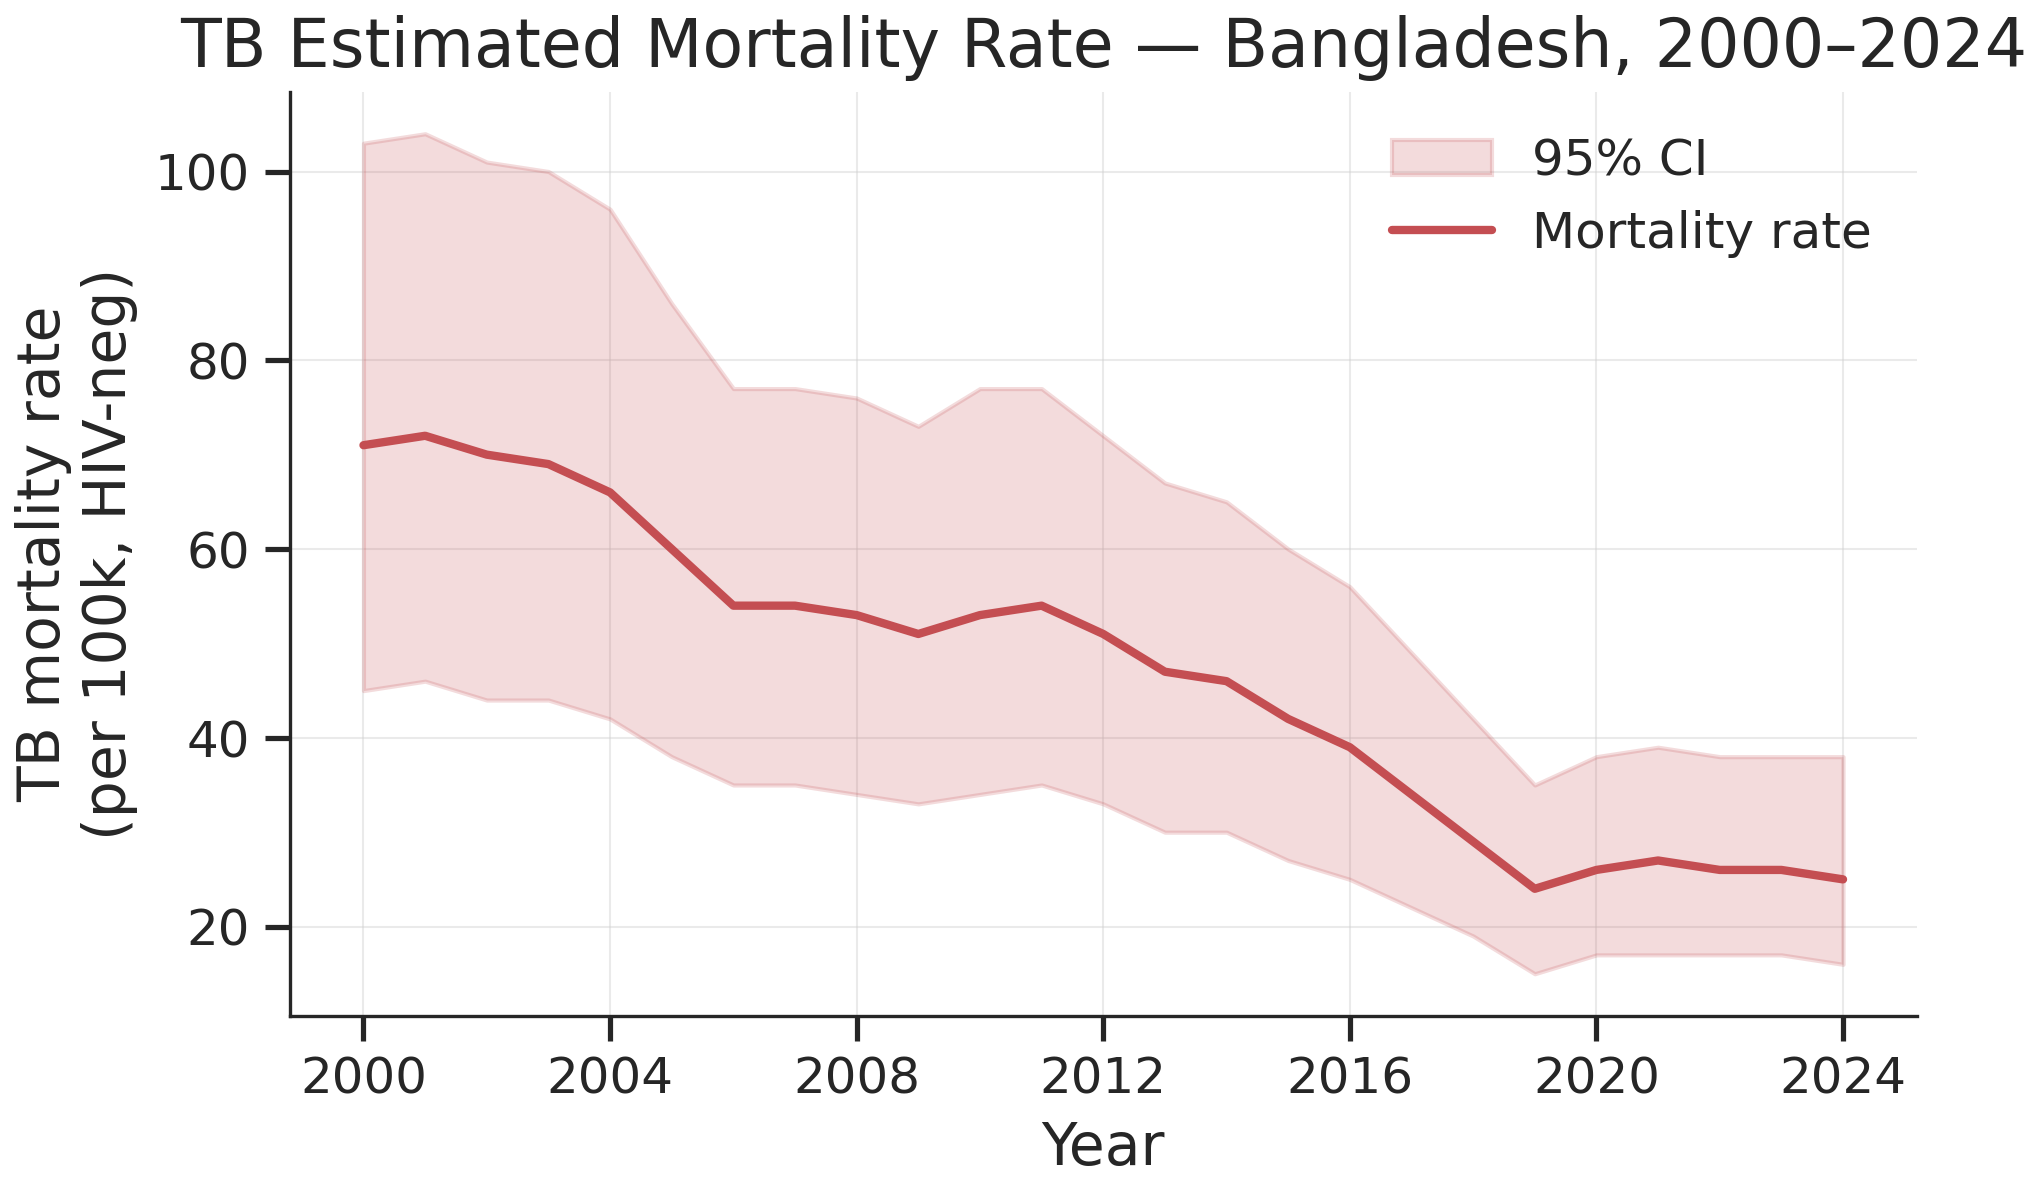
\includegraphics[width=\textwidth]{fig2_mortality_trend}
    \subcaption{Estimated TB mortality rate (per 100\,000, HIV-negative) with 95\,\%
      confidence interval.  Mortality fell from $\sim$75 to $\sim$27 per 100\,000,
      a $>$60\,\% decline over 25 years.}
    \label{fig:1b}
  \end{subfigure}
  \hfill
  \begin{subfigure}[t]{0.48\textwidth}
    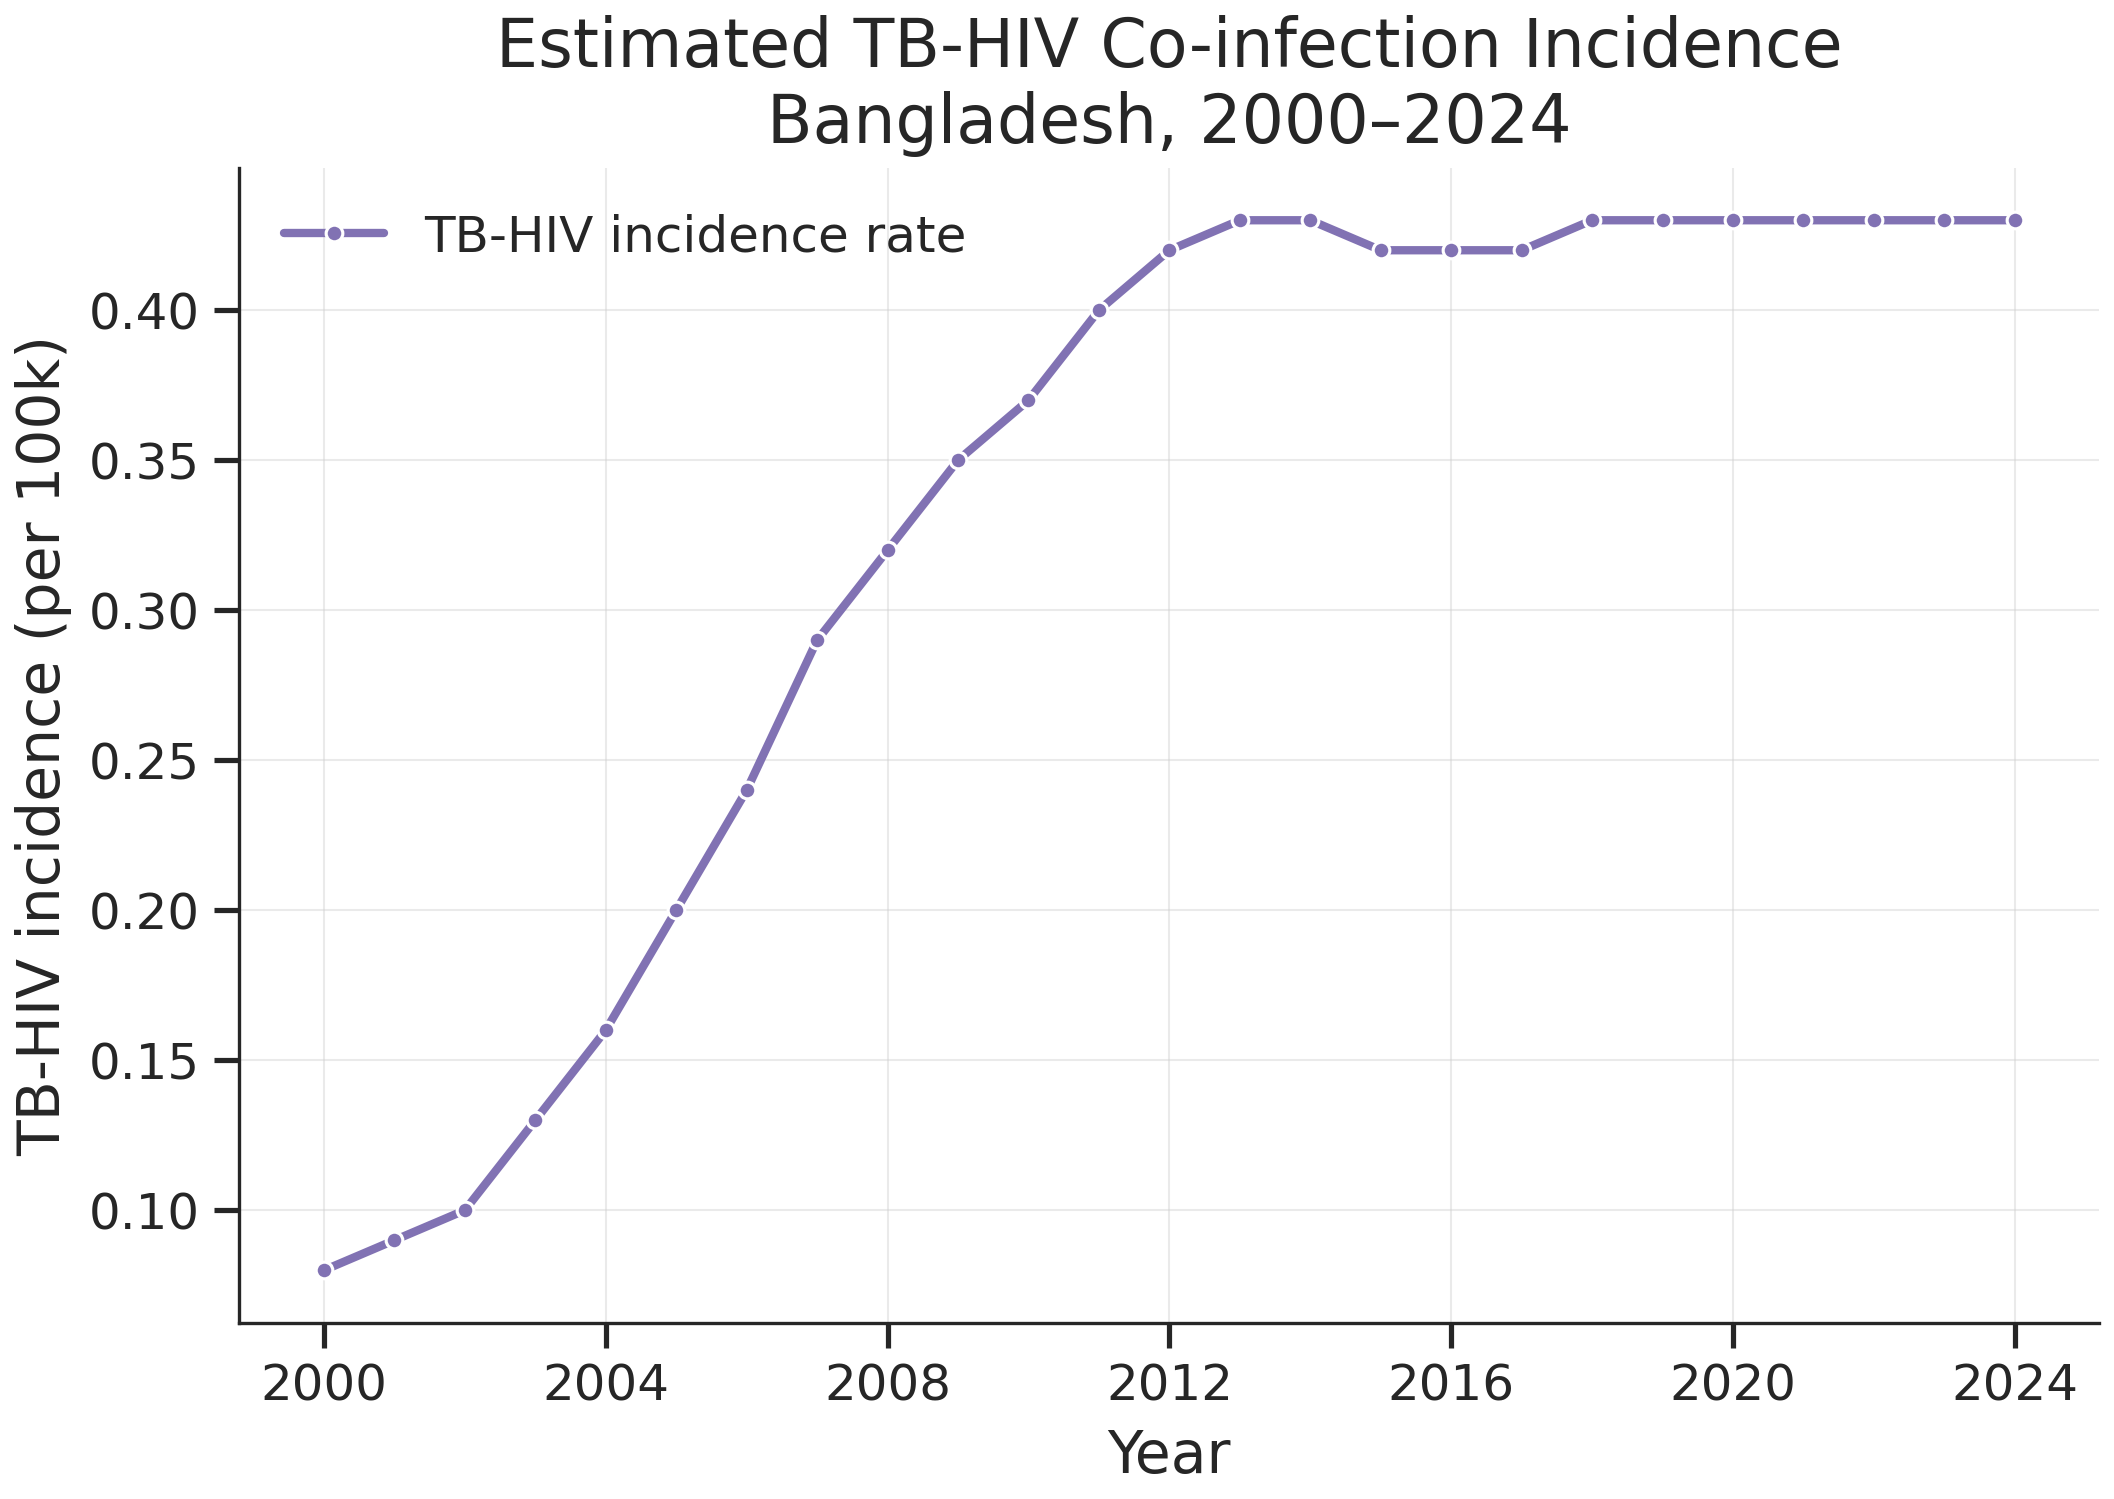
\includegraphics[width=\textwidth]{fig4_hivtb}
    \subcaption{Estimated TB-HIV co-infection incidence rate (per 100\,000).
      Bangladesh maintains HIV prevalence $<0.1$\,\%; the plateau since $\sim$2012
      reflects the low but stable co-infection background.}
    \label{fig:1c}
  \end{subfigure}
  \caption{\textbf{National TB epidemiological trends --- Bangladesh, 2000--2024.}
    Panel~(A) contextualises absolute burden against detection capacity;
    panels~(B) and~(C) track mortality and HIV co-infection trajectories.
    Together they establish the epidemiological arc of Bangladesh's TB response over 25 years.
    \textit{Source: WHO Global TB Programme burden estimates and notifications datasets.}}
  \label{fig:epi_trends}
\end{figure}
\clearpage

%% Figure 2 ─────────────────────────────────────────────────────────────────
\begin{figure}[htbp]
  \centering
  \begin{subfigure}[t]{0.56\textwidth}
    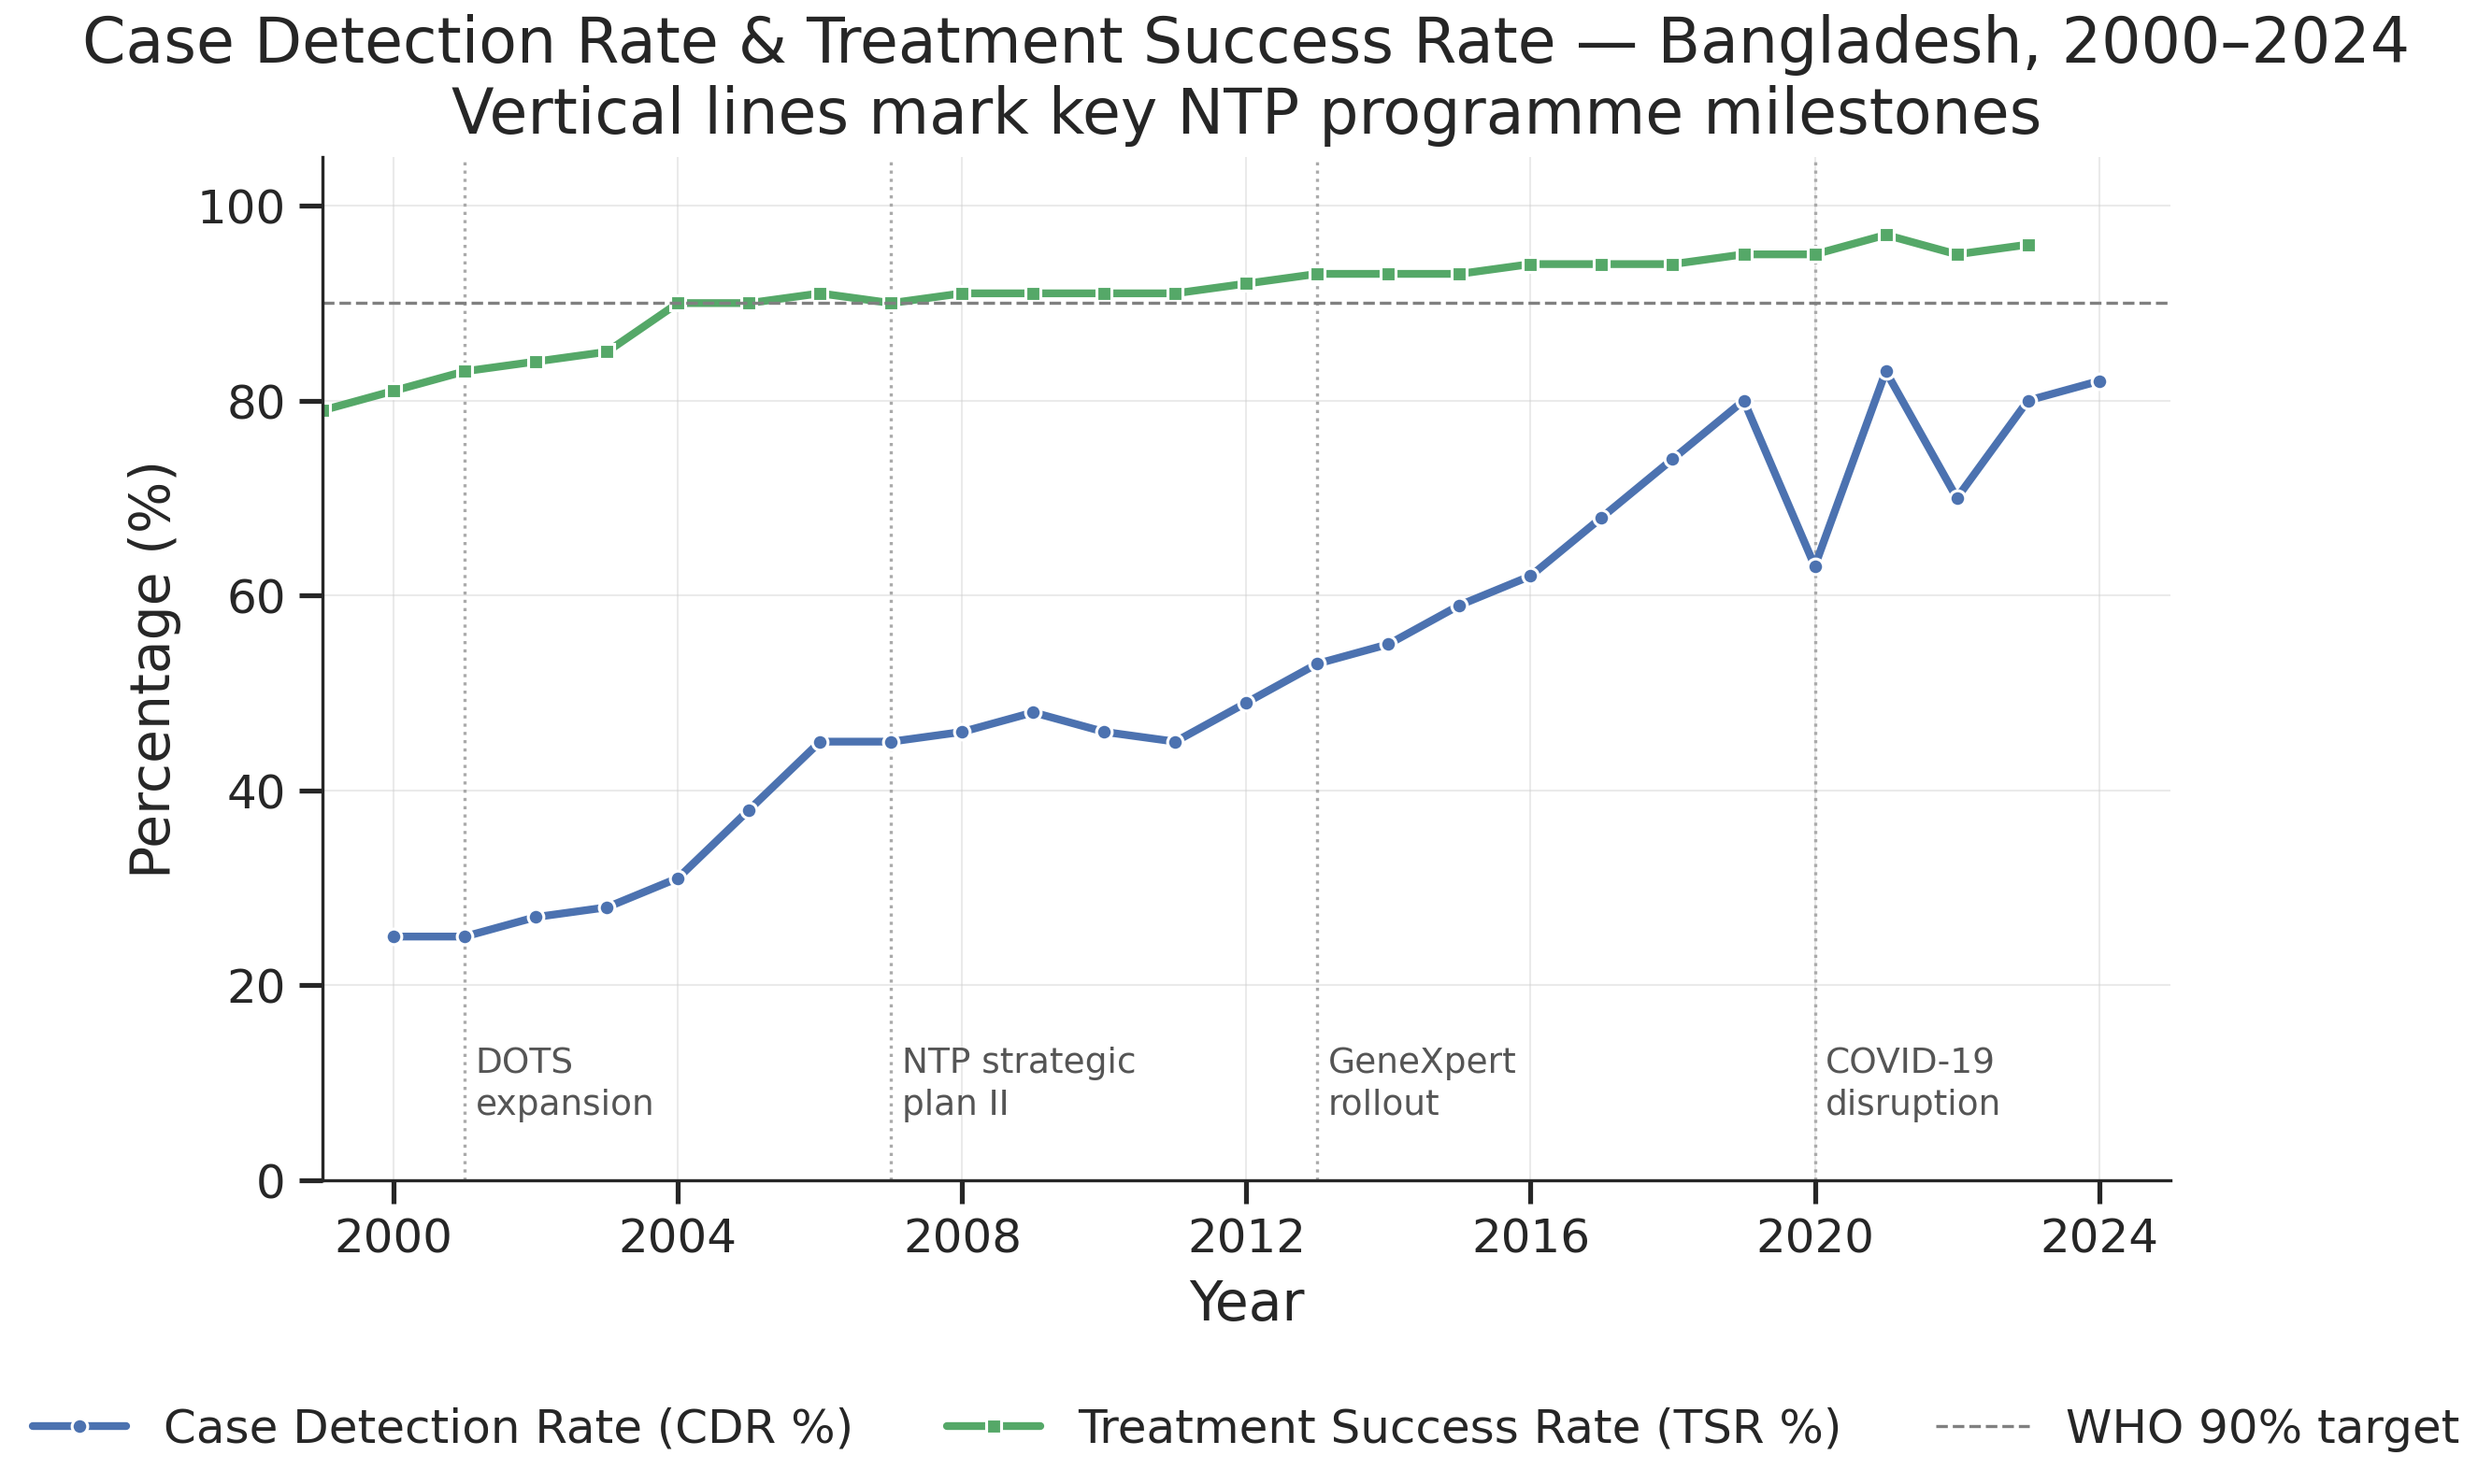
\includegraphics[width=\textwidth]{fig3_cdr_tsr}
    \subcaption{Case Detection Rate (CDR, \%) and Treatment Success Rate (TSR, \%)
      with key NTP programme milestones.  Bangladesh surpassed the WHO 90\,\%
      TSR target by 2009 and has sustained it since; CDR crossed 80\,\% in 2019
      before a COVID-19-related dip in 2020--21.}
    \label{fig:2a}
  \end{subfigure}
  \hfill
  \begin{subfigure}[t]{0.42\textwidth}
    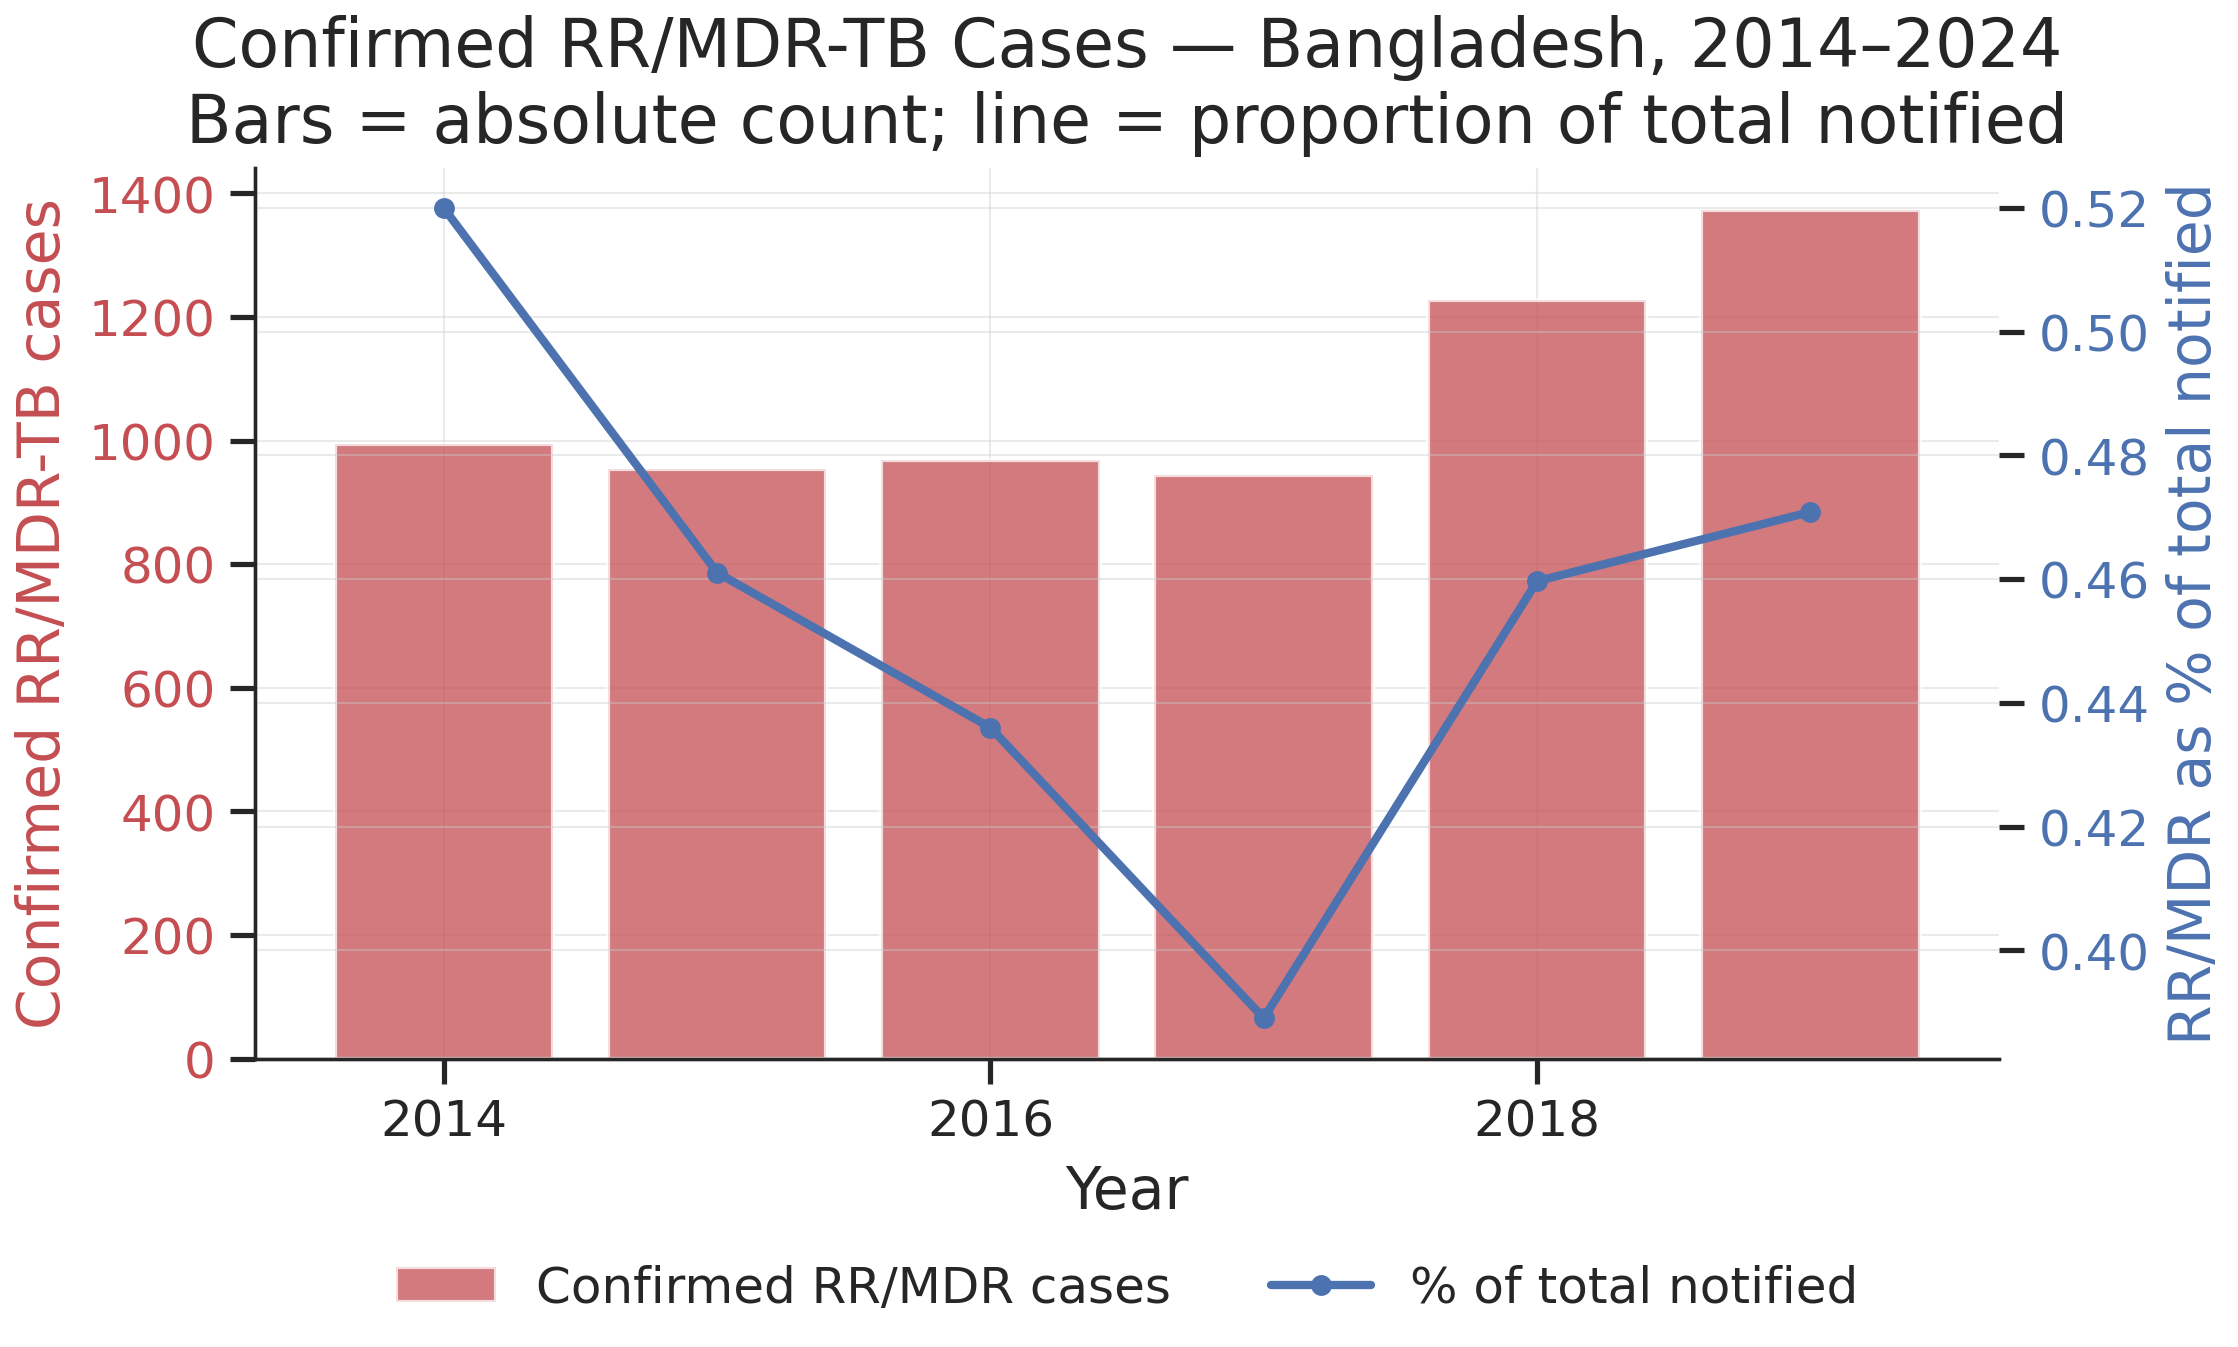
\includegraphics[width=\textwidth]{fig12_mdr_trend}
    \subcaption{Confirmed RR/MDR-TB cases (bars, left axis) and proportion of
      total notified cases (line, right axis), 2014--2024.
      Absolute case counts have risen despite a declining proportion,
      signalling an absolute drug-resistance burden that requires sustained vigilance.}
    \label{fig:2b}
  \end{subfigure}
  \caption{\textbf{National TB programme performance --- Bangladesh, 2000--2024.}
    Panel~(A) shows the trajectory of case-finding and treatment success alongside
    the four pivotal NTP milestones (DOTS expansion 2001, strategic plan II 2007,
    GeneXpert rollout 2013, COVID-19 disruption 2020).
    Panel~(B) tracks the emerging drug-resistance challenge.
    Both indicators are prerequisites for achieving WHO End-TB targets by 2030.
    \textit{Source: WHO Global TB Programme.}}
  \label{fig:prog_perf}
\end{figure}
\clearpage

%% Figure 3 ─────────────────────────────────────────────────────────────────
\begin{figure}[htbp]
  \centering
  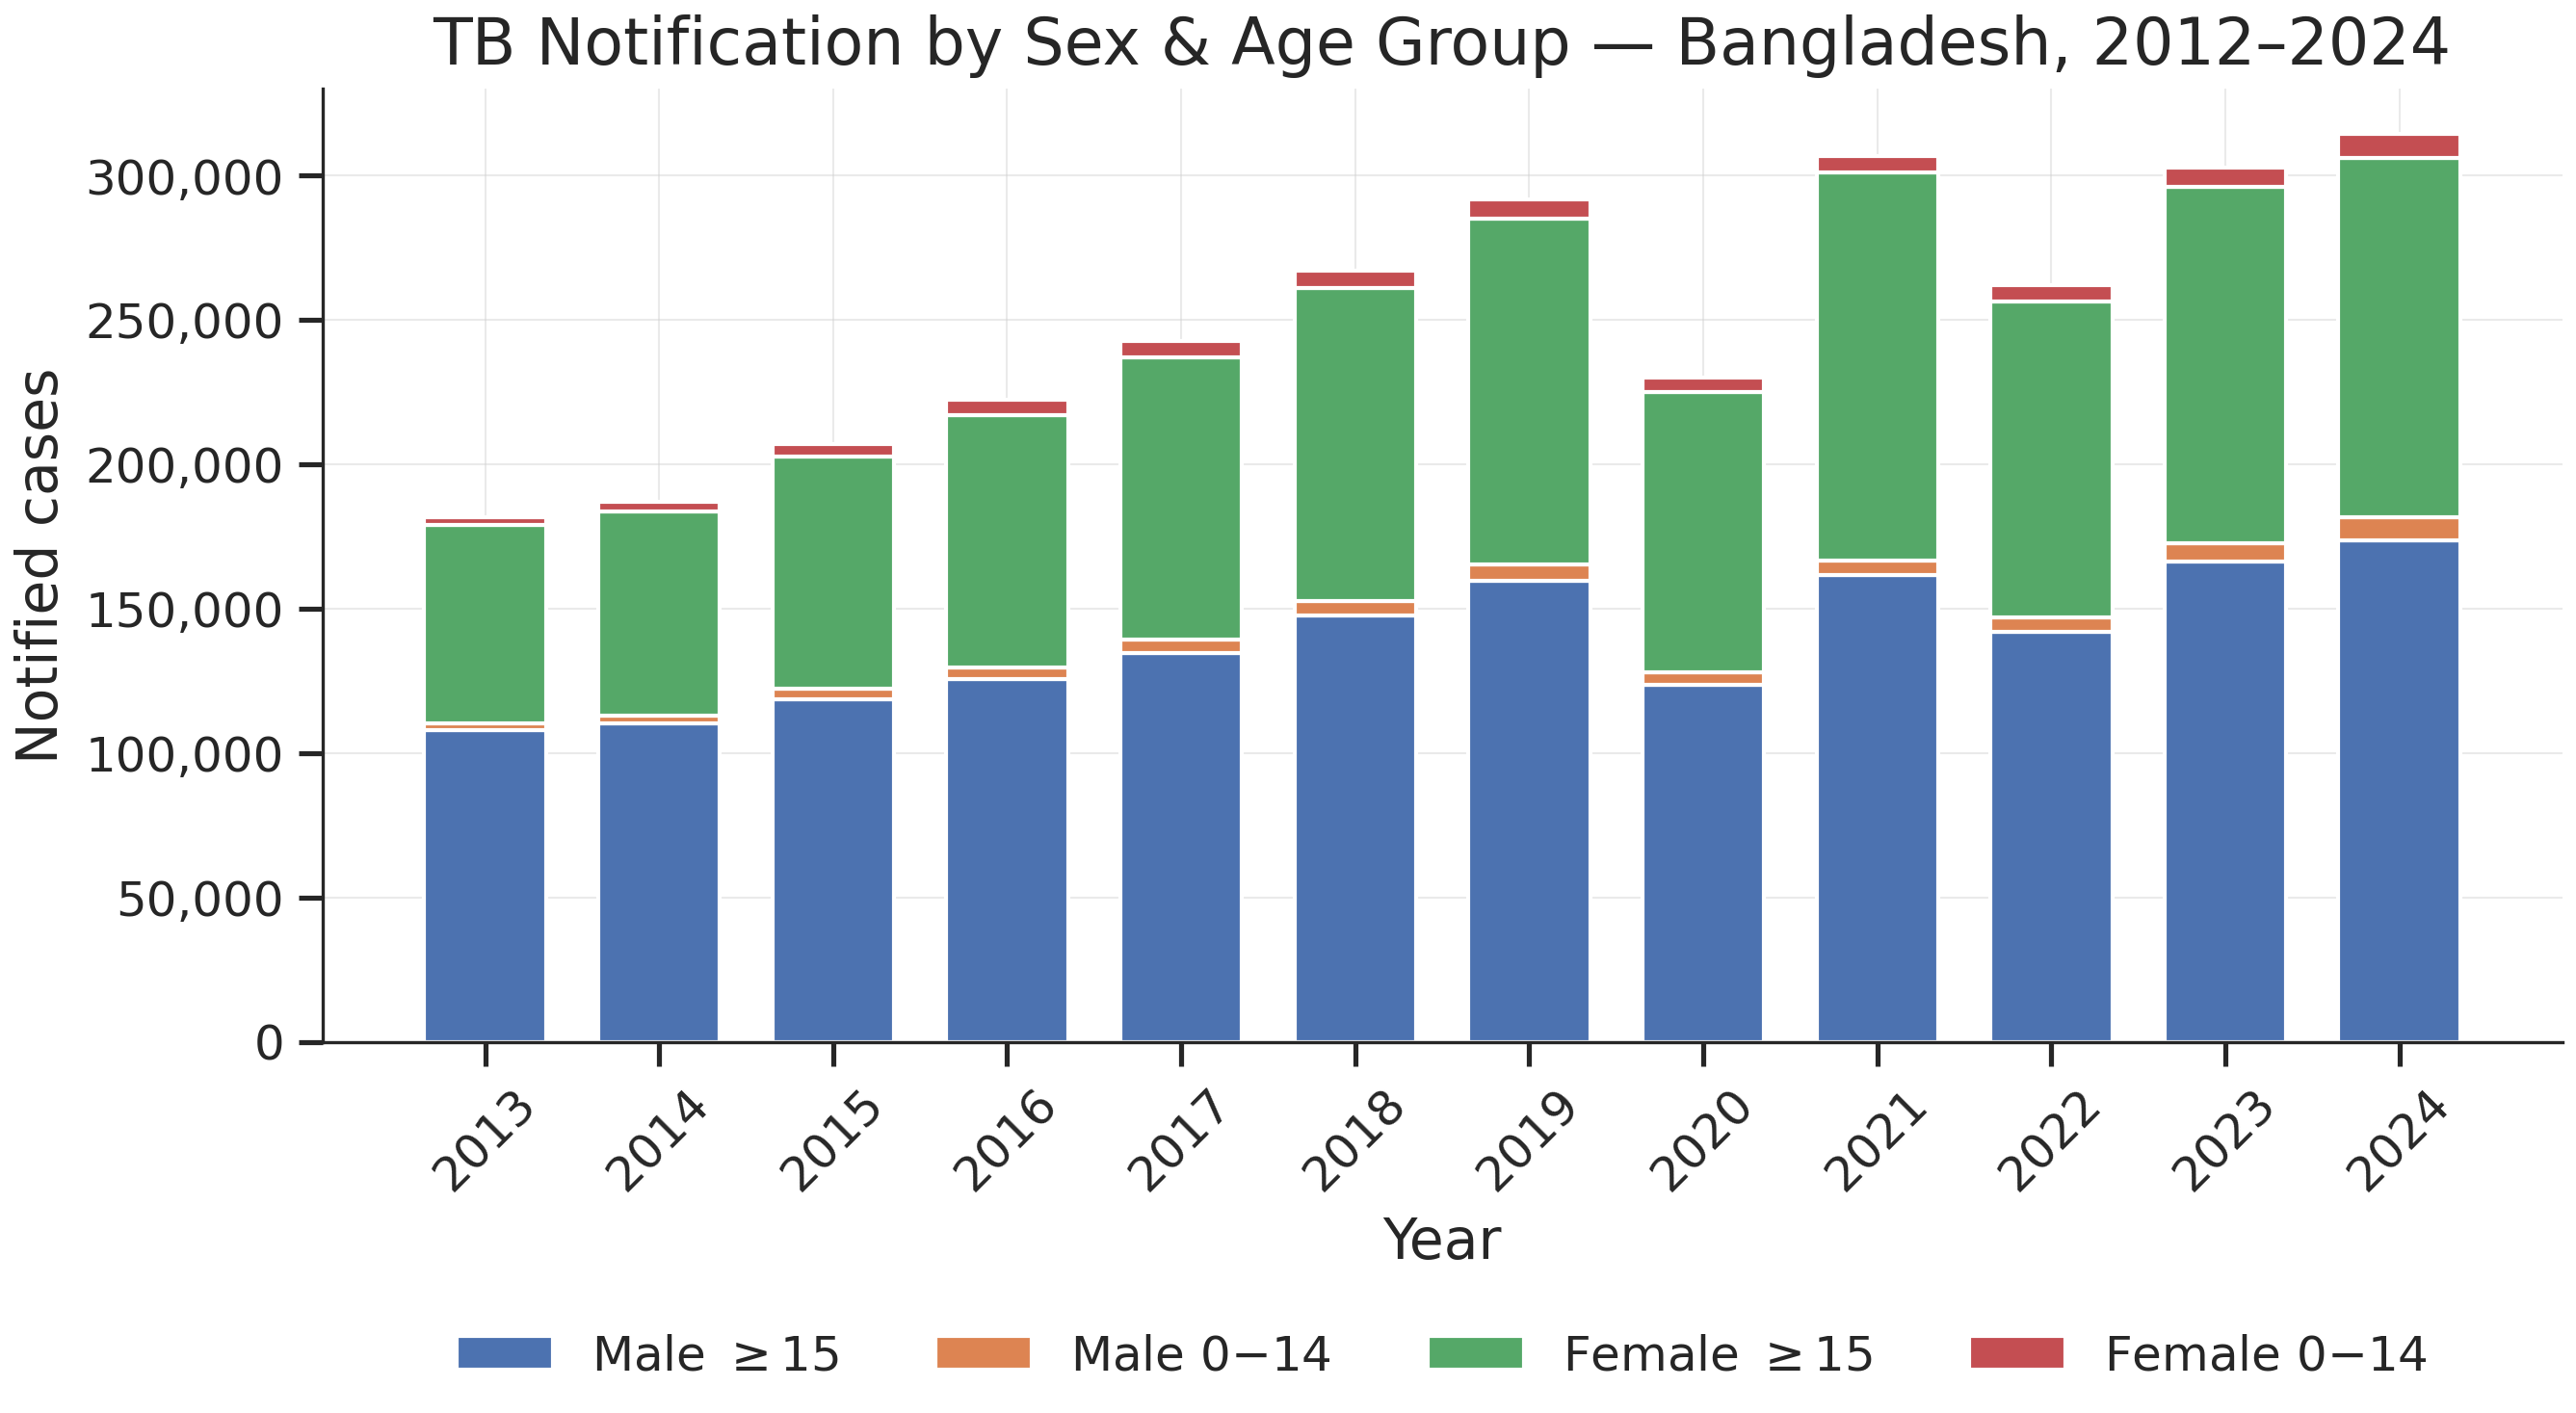
\includegraphics[width=\textwidth]{fig5_sex_age_distribution}
  \caption{\textbf{TB notifications by sex and age group --- Bangladesh, 2012--2024.}
    Stacked bars show four demographic strata: males $\geq$15 (dominant stratum, blue),
    females $\geq$15 (green), males 0--14 (orange), and females 0--14 (red).
    Adult males consistently account for $\sim$55\,\% of all notifications,
    consistent with the global pattern of higher TB exposure and prevalence in working-age men.
    The decline in 2020 reflects COVID-19-related health-service disruption;
    the subsequent rebound demonstrates programme resilience.
    Sex- and age-disaggregated data available from 2012 onward.
    \textit{Source: WHO Global TB Programme notifications dataset.}}
  \label{fig:demographics}
\end{figure}
\clearpage

%% Figure 4 ─────────────────────────────────────────────────────────────────
\begin{figure}[htbp]
  \centering
  \begin{subfigure}[t]{\textwidth}
    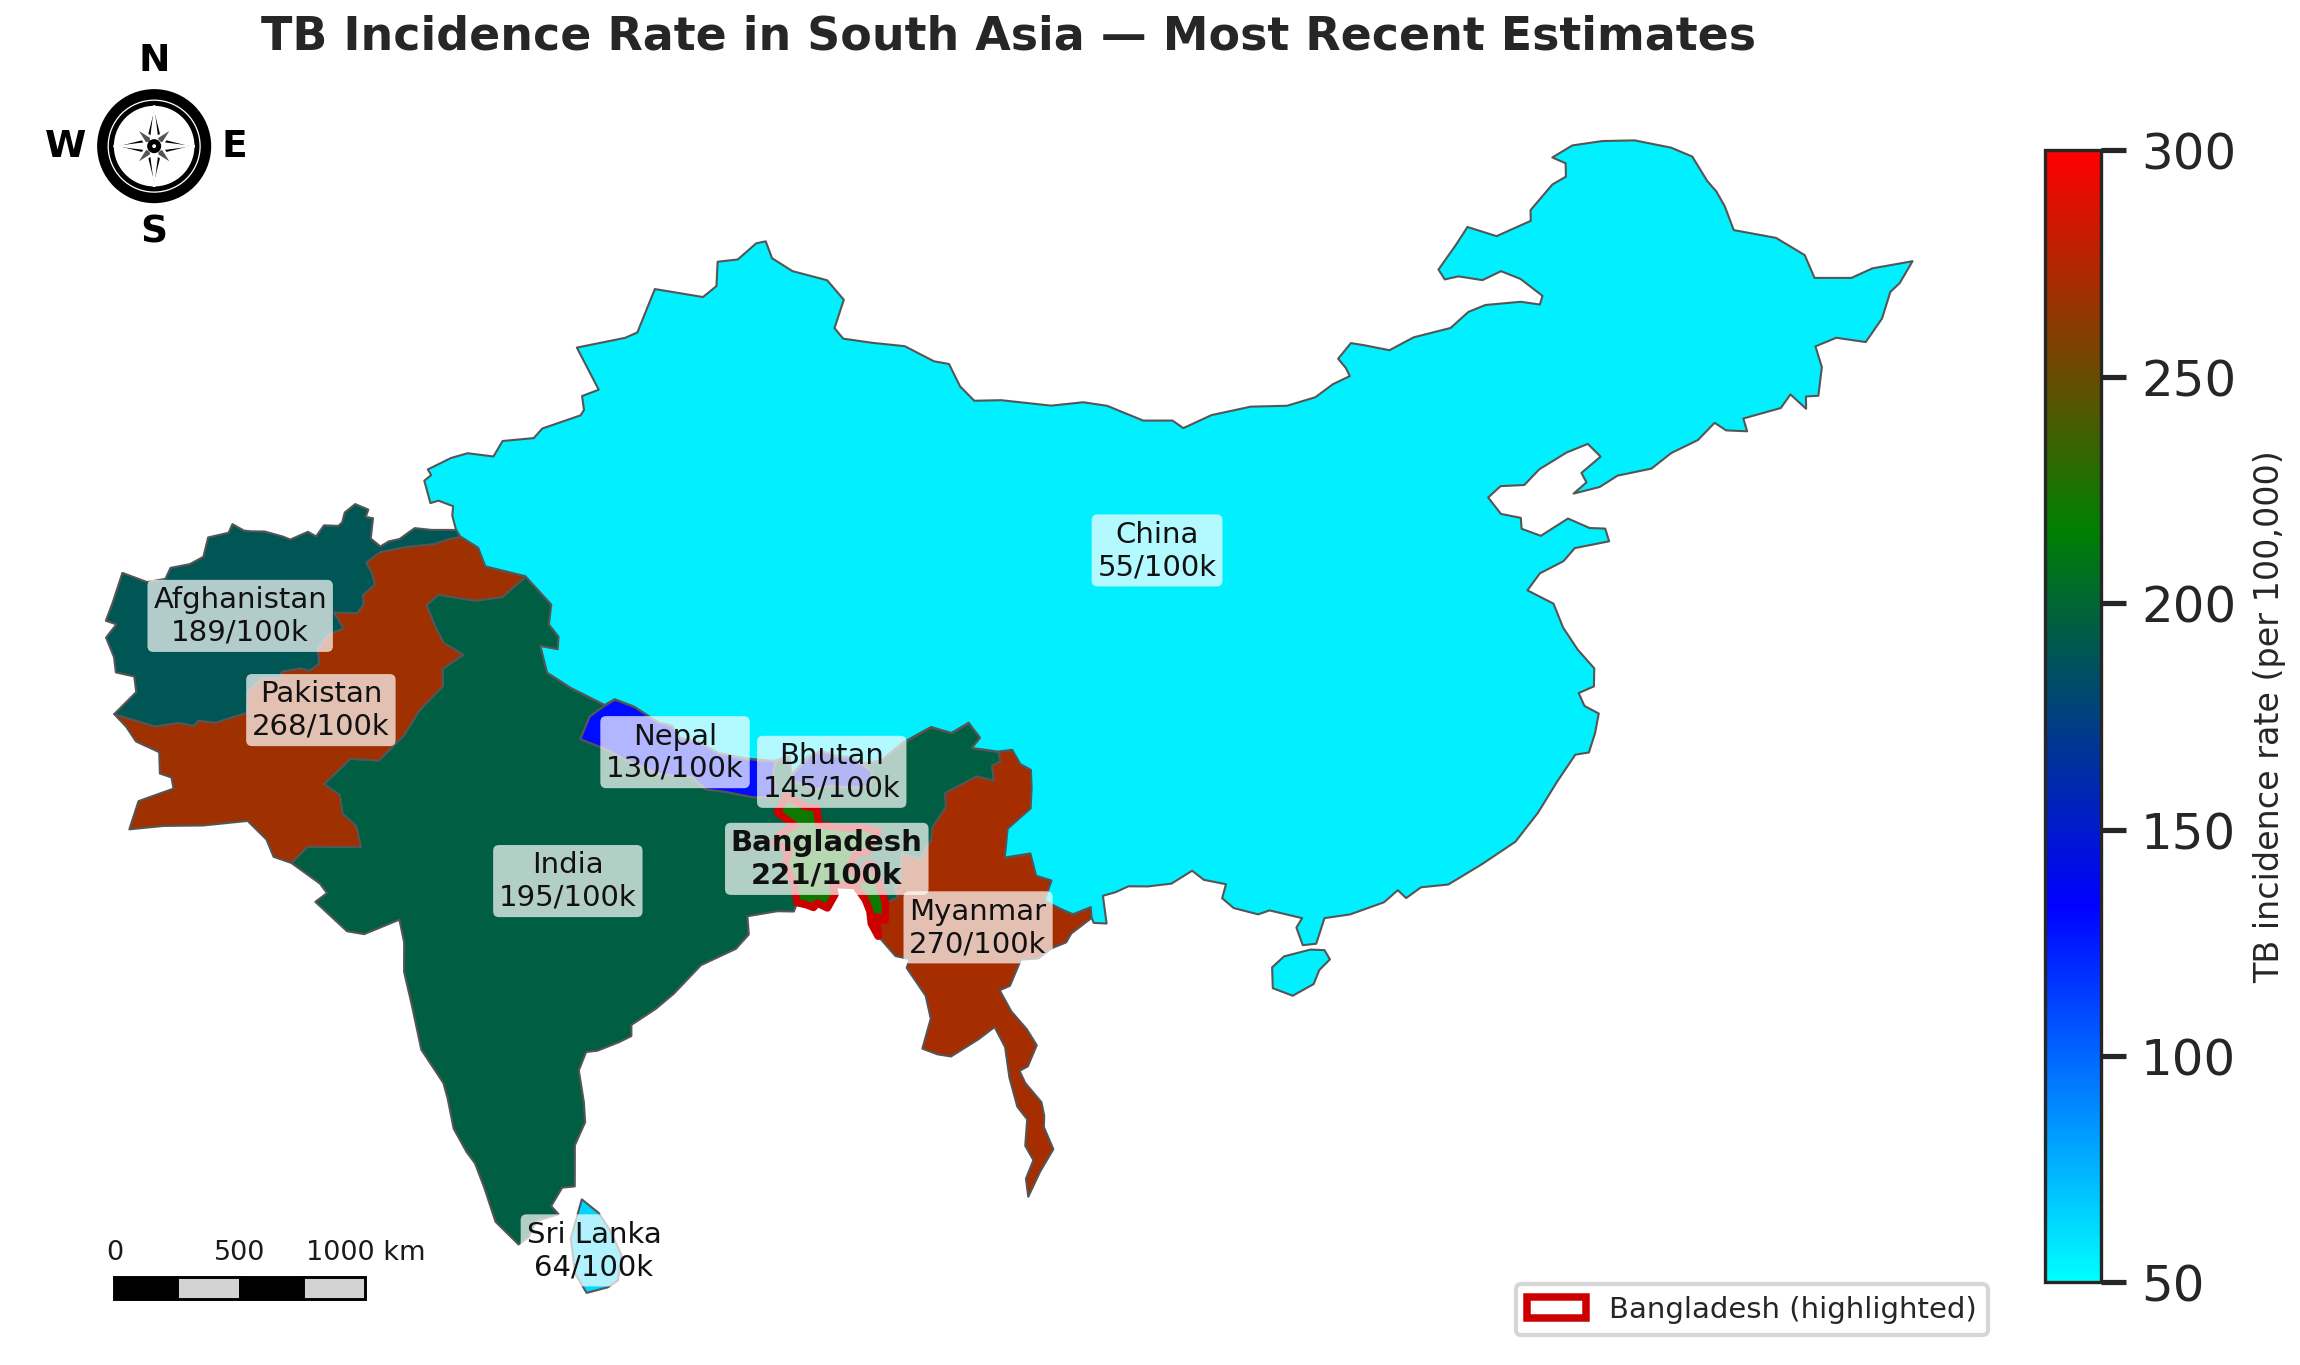
\includegraphics[width=\textwidth, height=0.28\textheight, keepaspectratio]{map5_south_asia_context}
    \subcaption{TB incidence rate (per 100\,000) across South and Southeast Asia ---
      most recent WHO estimates.  Bangladesh (red border) carries one of the region's
      highest absolute burdens, second only to India in total case count,
      yet its incidence rate is lower than several neighbouring countries.}
    \label{fig:4a}
  \end{subfigure}
  \vspace{0.8em}
  \begin{subfigure}[t]{0.50\textwidth}
    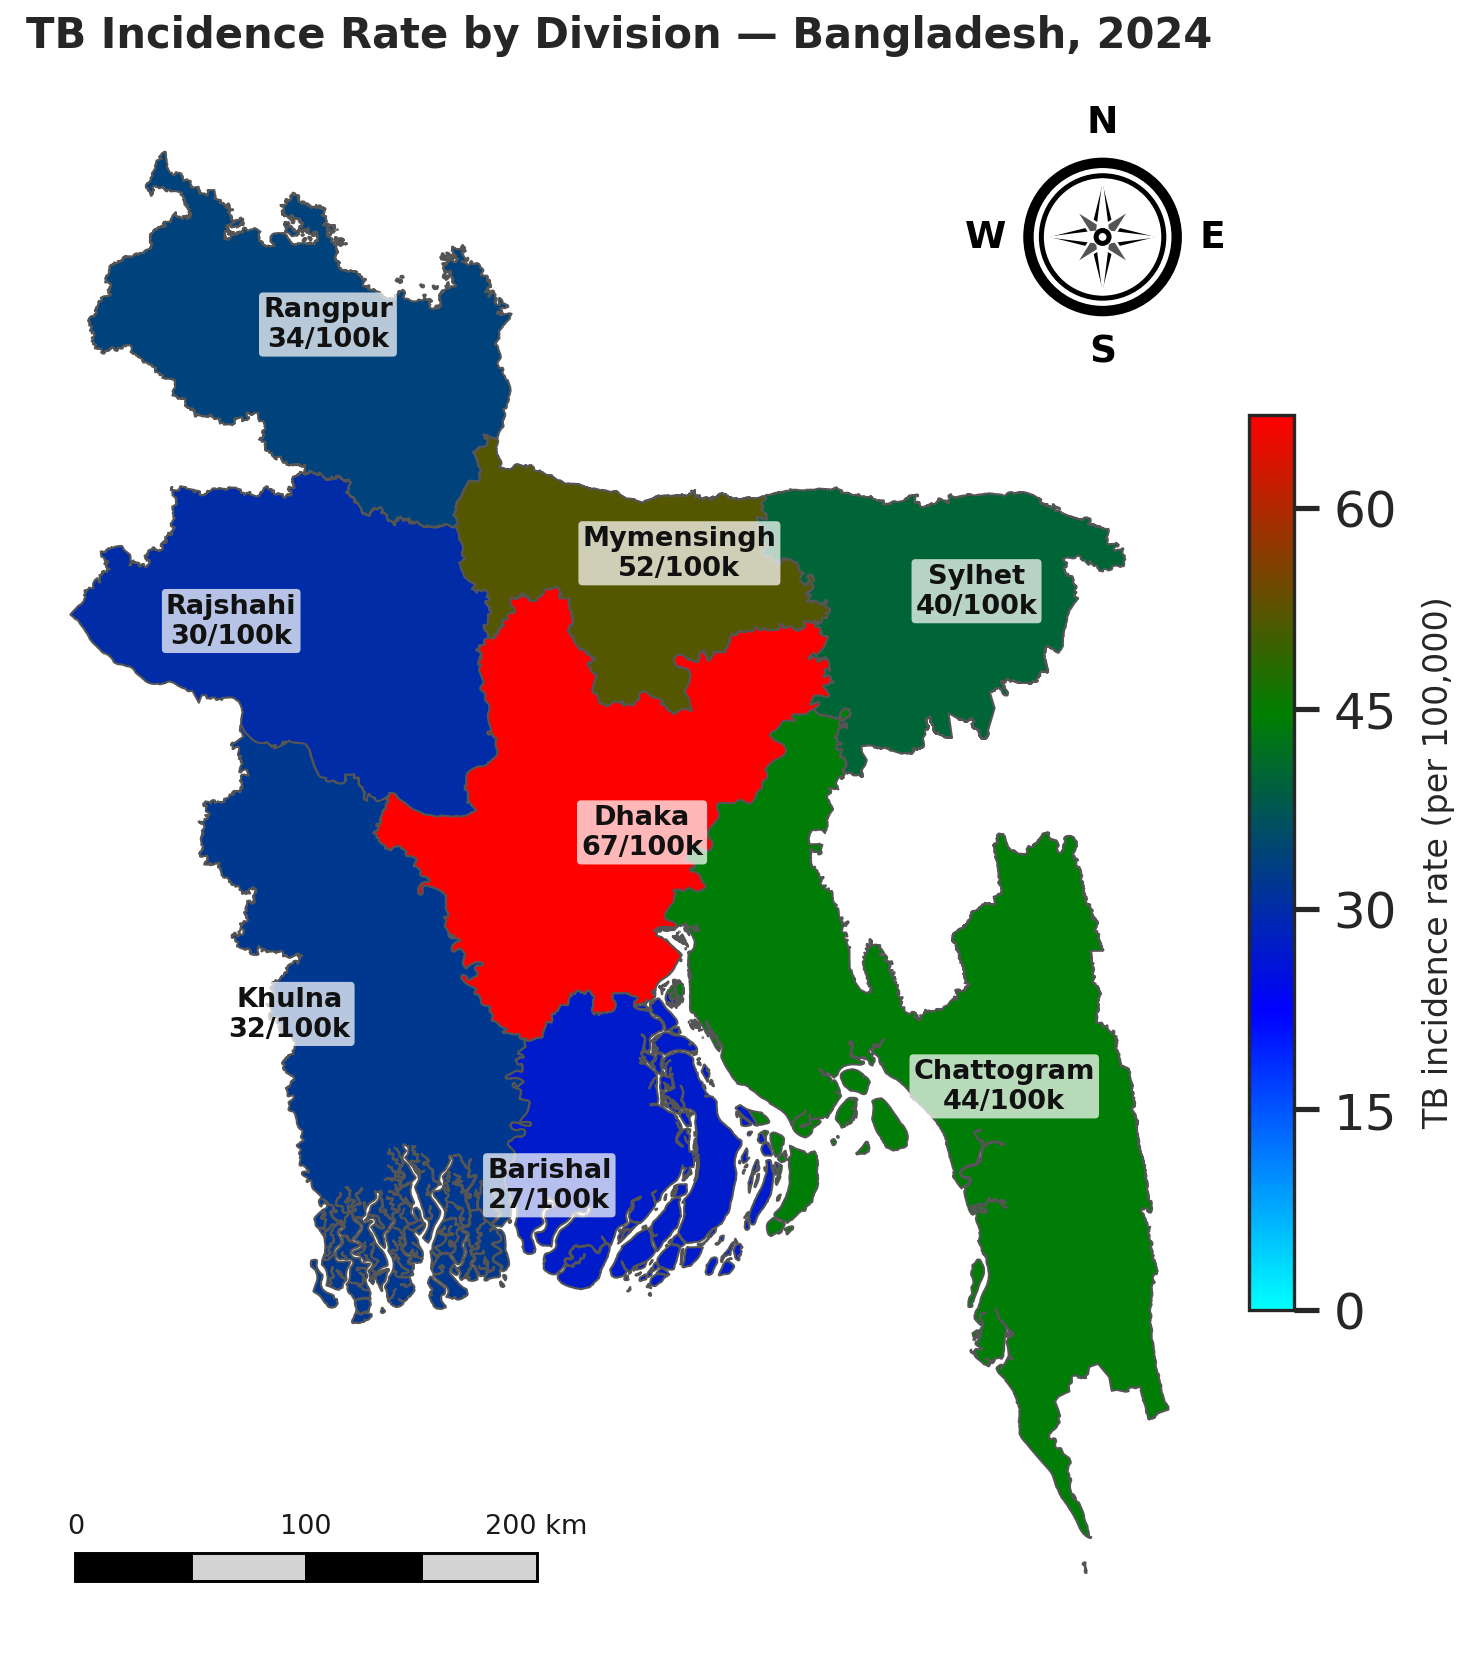
\includegraphics[width=\textwidth, height=0.30\textheight, keepaspectratio]{map4_incidence_2024}
    \subcaption{Division-level TB incidence rate (per 100\,000) --- Bangladesh, 2024.
      Dhaka and Chattogram divisions record the highest rates,
      driven by population density and urban migration.}
    \label{fig:4b}
  \end{subfigure}
  \hfill
  \begin{subfigure}[t]{0.46\textwidth}
    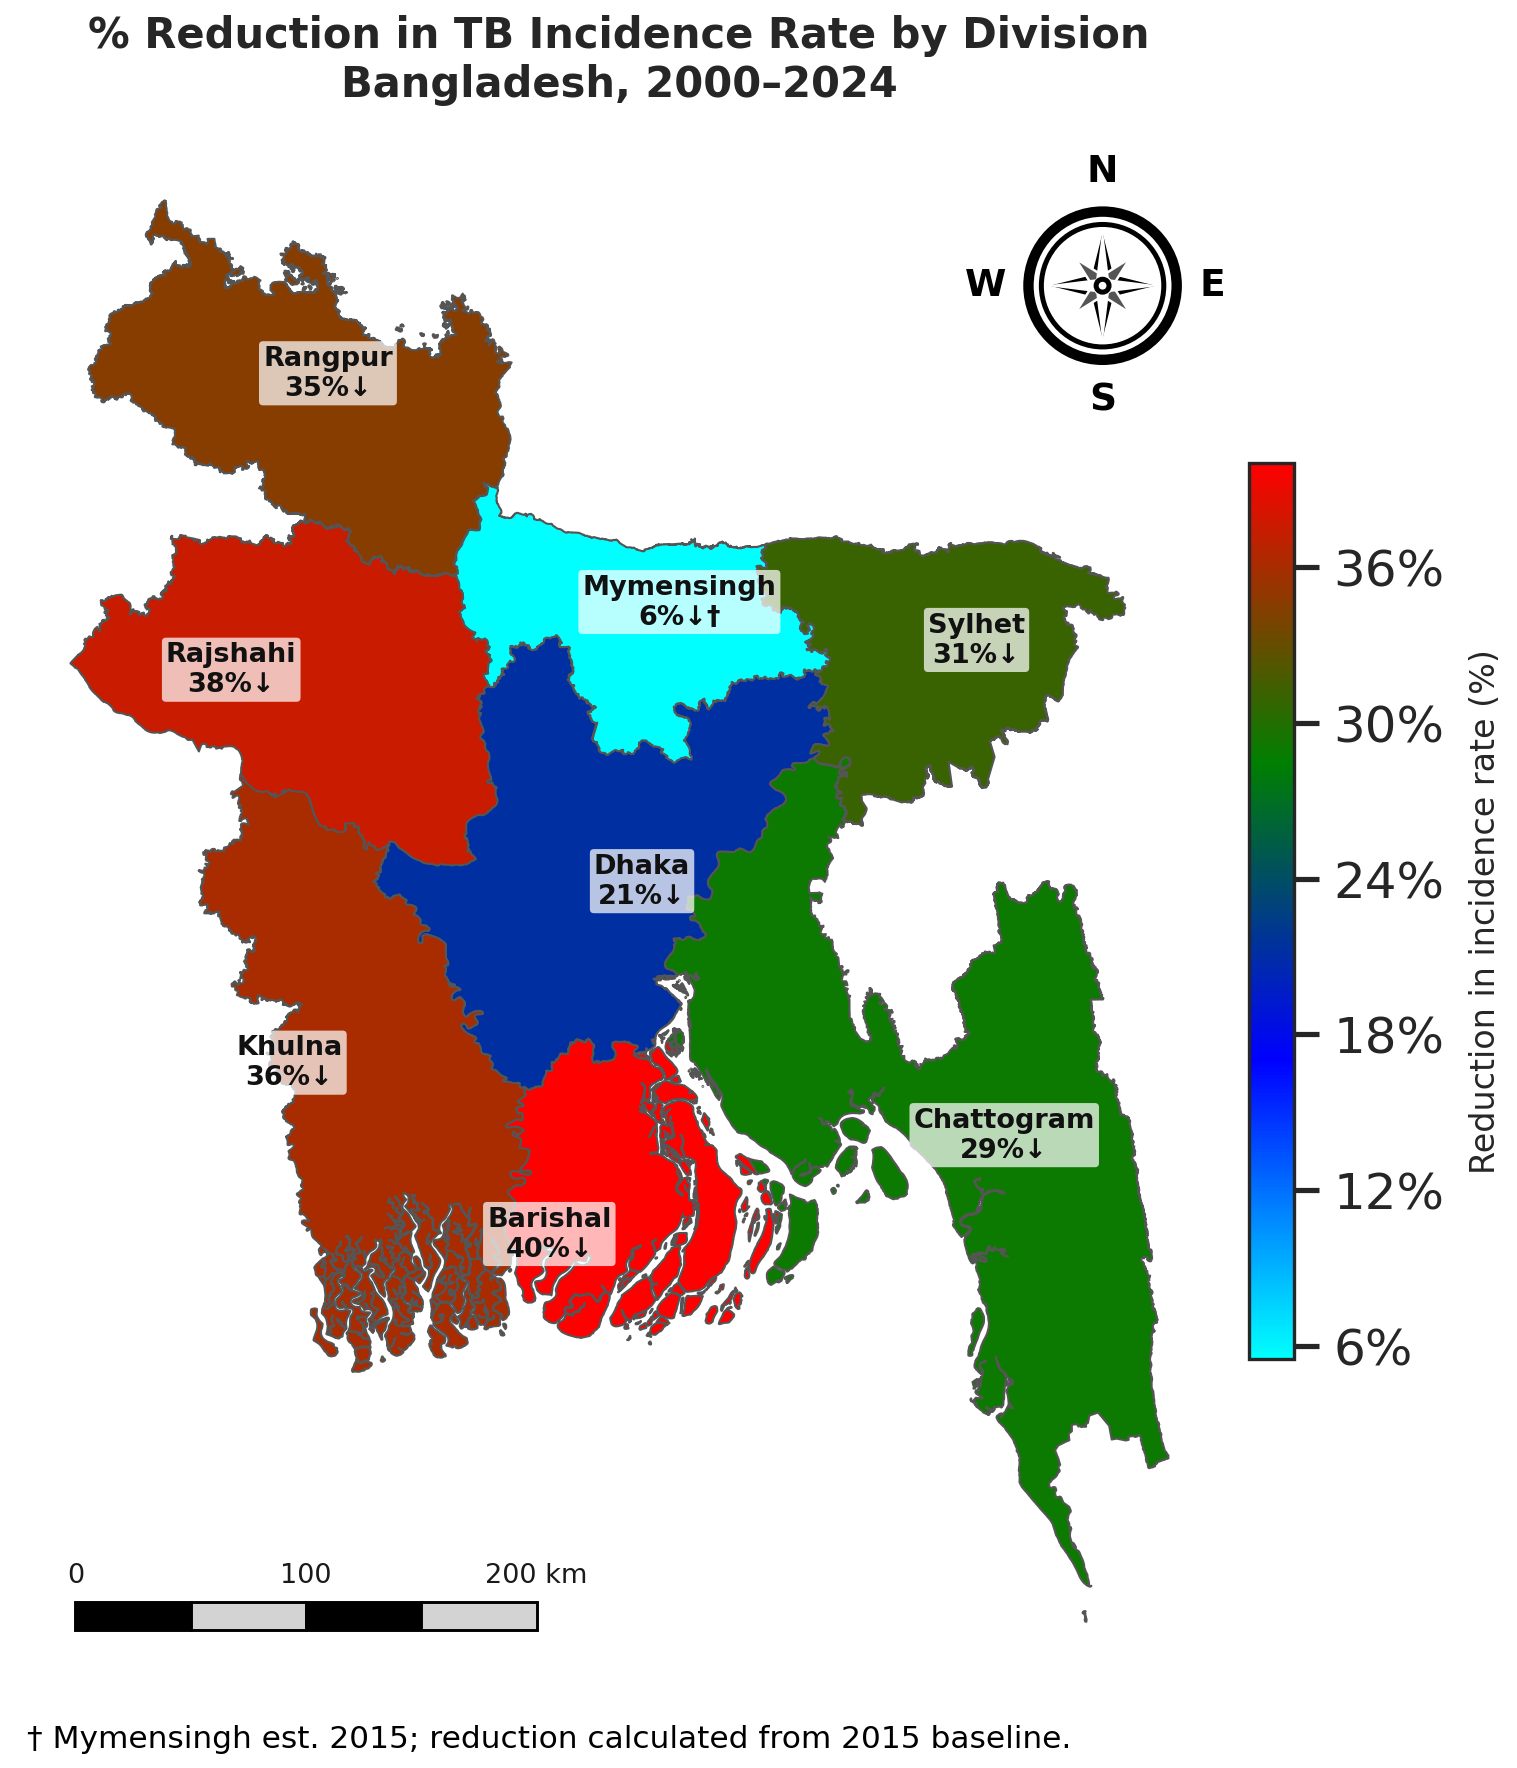
\includegraphics[width=\textwidth, height=0.30\textheight, keepaspectratio]{map6_incidence_reduction}
    \subcaption{Proportional reduction in TB incidence rate by division, 2000$\to$2024.
      Greener shading indicates greater improvement.
      $\dagger$Mymensingh division established 2015; reduction calculated from 2015 baseline.}
    \label{fig:4c}
  \end{subfigure}
  \caption{\textbf{Geographic distribution of TB burden --- regional context and within-country variation.}
    Panel~(A) situates Bangladesh within the South Asian high-burden region.
    Panel~(B) shows the within-country distribution in 2024, highlighting
    the urban concentration of disease.
    Panel~(C) quantifies progress: all divisions achieved at least a 4\,\% reduction,
    but the magnitude varies substantially, pointing to persistent geographic inequities.
    \textit{Sources: WHO Global TB Programme; NTP Bangladesh / DGHS Annual Reports;
    Natural Earth 1:110m boundaries; OCHA HDX Bangladesh Admin Boundaries.}}
  \label{fig:geo_dist}
\end{figure}
\clearpage

%% Figure 5 ─────────────────────────────────────────────────────────────────
\begin{figure}[htbp]
  \centering
  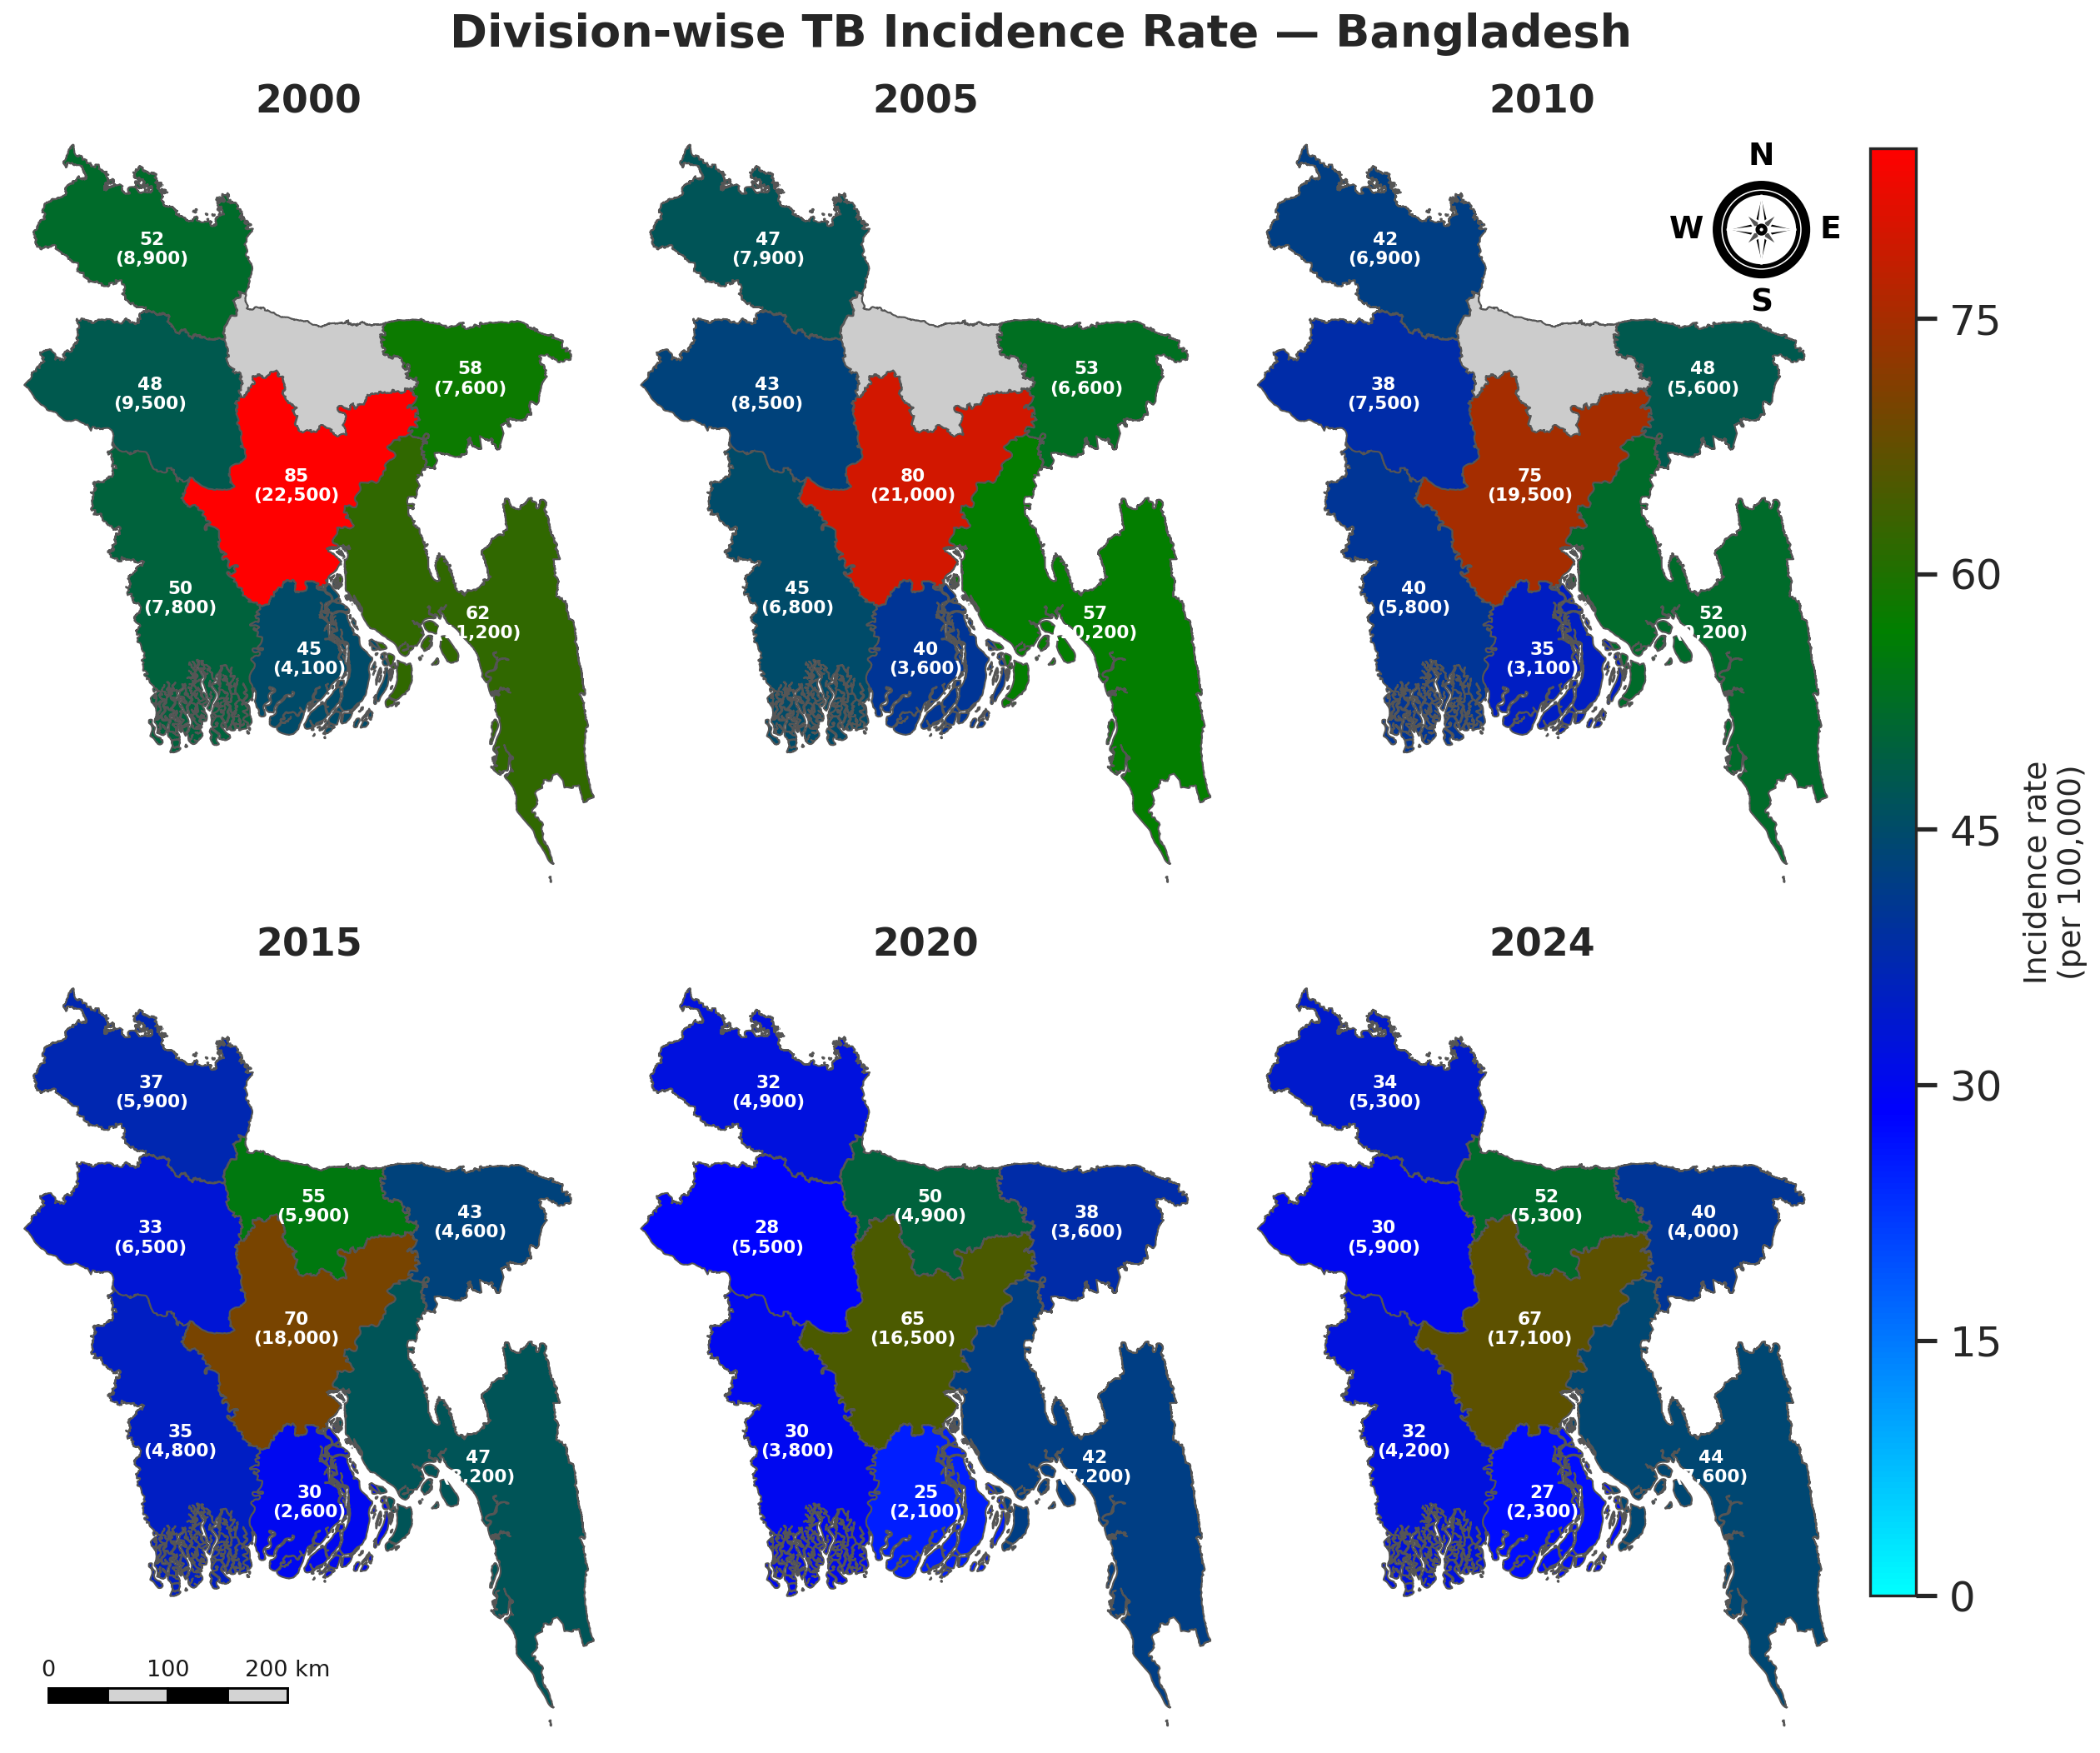
\includegraphics[width=\textwidth]{map3_incidence_small_multiples}
  \caption{\textbf{Division-wise TB incidence rate (per 100\,000) at key years ---
    Bangladesh, 2000--2024.}
    Each panel label shows both the incidence rate and absolute notified case count.
    The progression from 2000 to 2024 illustrates the uneven pace of decline:
    Dhaka consistently leads in absolute burden; Mymensingh appears from 2015
    (carved from Dhaka division); all divisions show declining rates by 2020--24,
    accelerated by intensified case-finding efforts.
    \textit{Source: NTP Bangladesh / DGHS Annual Reports.}}
  \label{fig:geo_temporal}
\end{figure}
\clearpage

%% Figure 6 ─────────────────────────────────────────────────────────────────
\begin{figure}[htbp]
  \centering
  \begin{subfigure}[t]{\textwidth}
    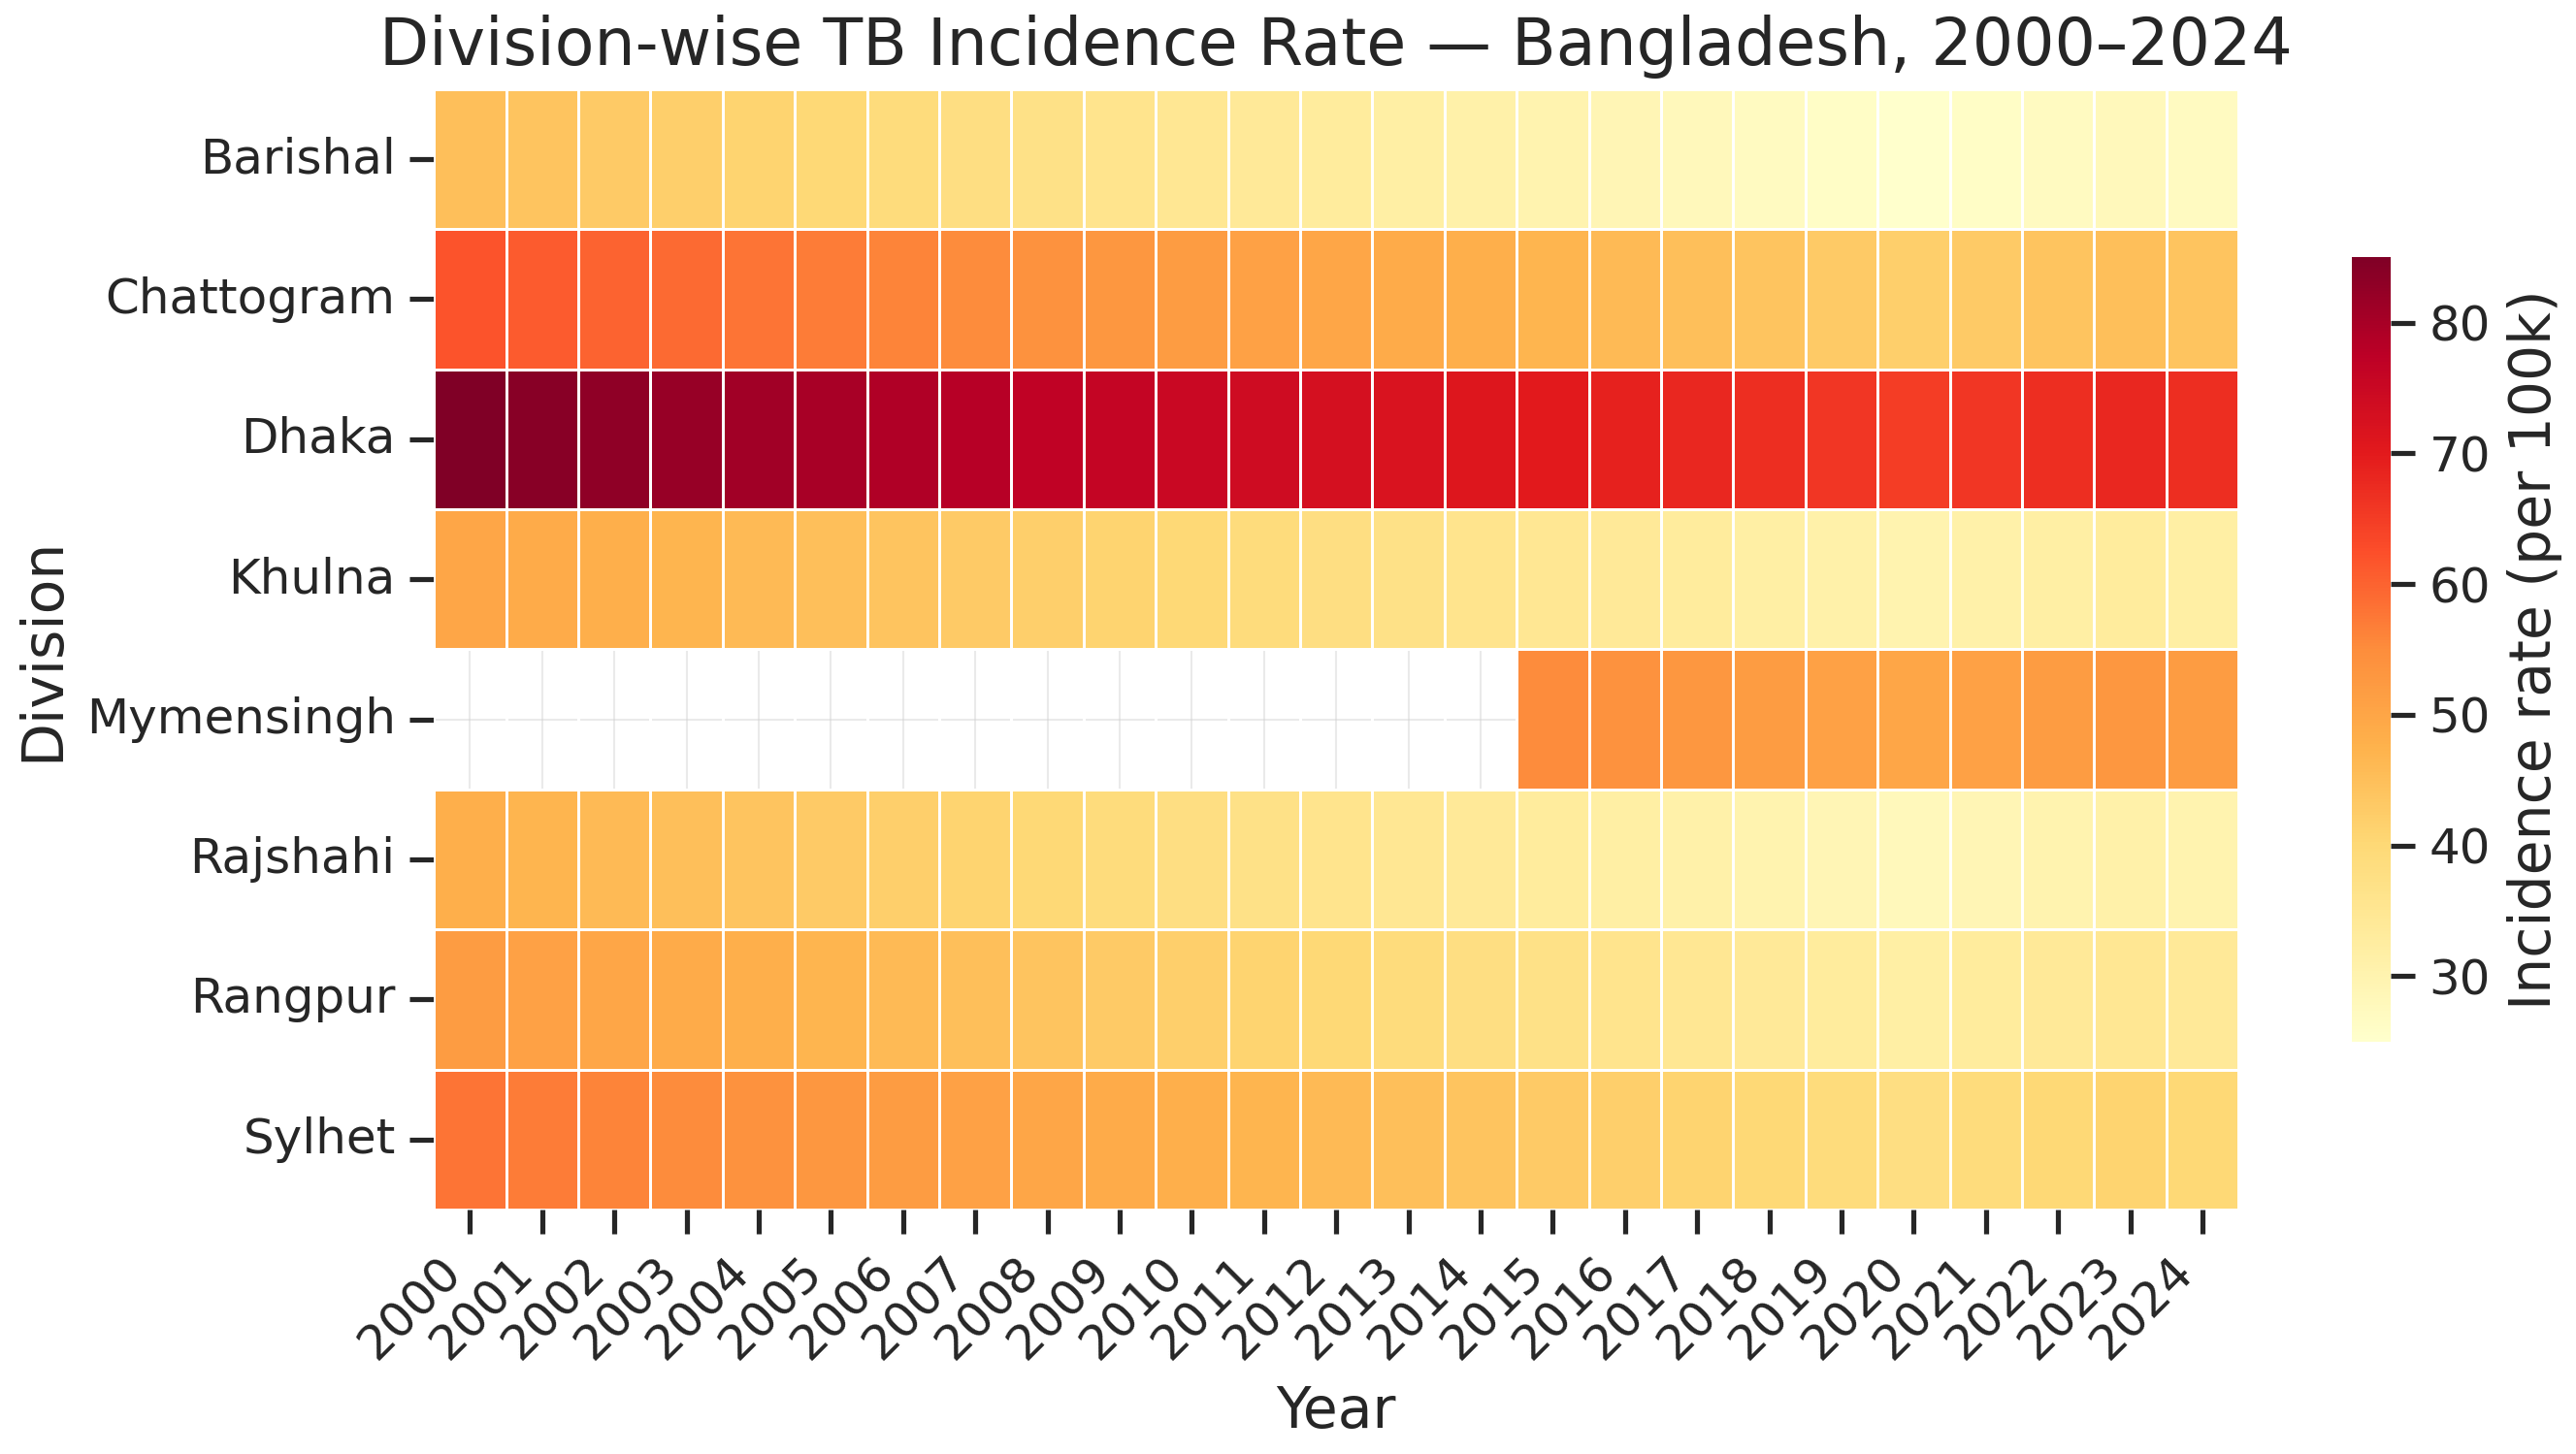
\includegraphics[width=\textwidth]{fig6_division_heatmap}
    \subcaption{Division-wise TB incidence rate heatmap, 2000--2024.
      Colour intensity encodes incidence per 100\,000.
      Dhaka (darkest) has remained the highest-burden division throughout;
      Mymensingh data begin in 2015.}
    \label{fig:6a}
  \end{subfigure}
  \vspace{0.8em}
  \begin{subfigure}[t]{\textwidth}
    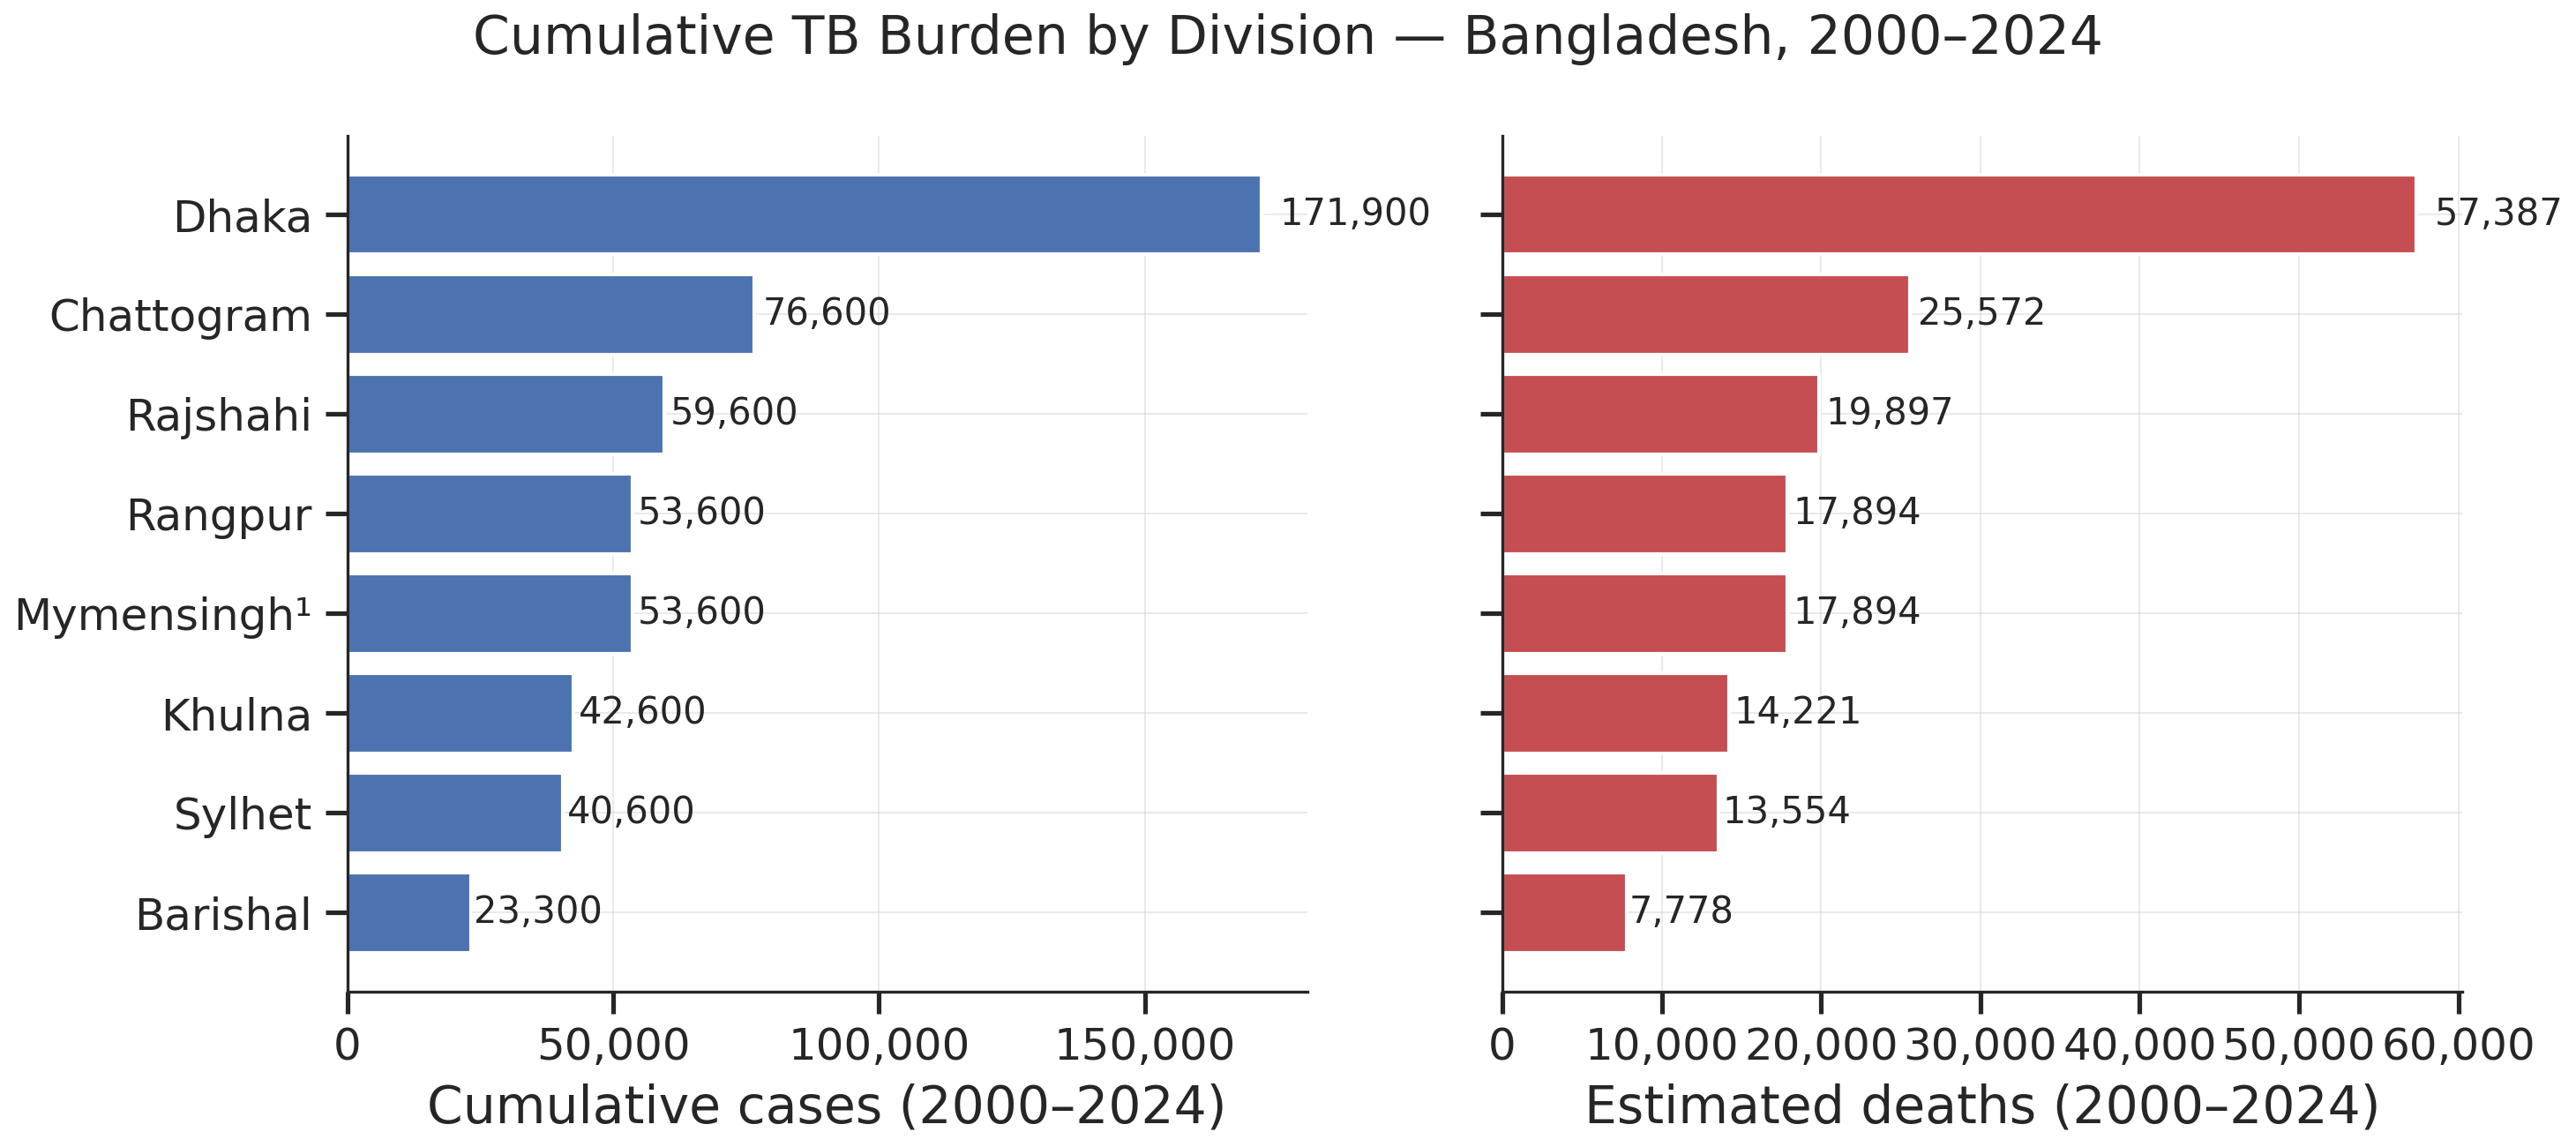
\includegraphics[width=\textwidth]{fig7_division_cumulative}
    \subcaption{Cumulative TB cases (left) and estimated deaths (right) by division,
      2000--2024, sorted by descending case count.
      Dhaka accounts for $\sim$28\,\% of all cumulative cases;
      together Dhaka and Chattogram represent nearly half the national burden.}
    \label{fig:6b}
  \end{subfigure}
  \caption{\textbf{Division-level TB burden --- temporal heatmap and cumulative summary,
    Bangladesh 2000--2024.}
    Panel~(A) reveals year-on-year trends within each division;
    panel~(B) converts those trends into cumulative burden for direct comparison
    across the eight administrative units.
    The contrast between Dhaka and Barishal ($\sim$7$\times$ difference in cumulative cases)
    underscores the need for geographically targeted resource allocation.
    \textit{Source: NTP Bangladesh / DGHS Annual Reports.}}
  \label{fig:div_burden}
\end{figure}
\clearpage

%% Figure 7 ─────────────────────────────────────────────────────────────────
\begin{figure}[htbp]
  \centering
  \begin{subfigure}[t]{0.48\textwidth}
    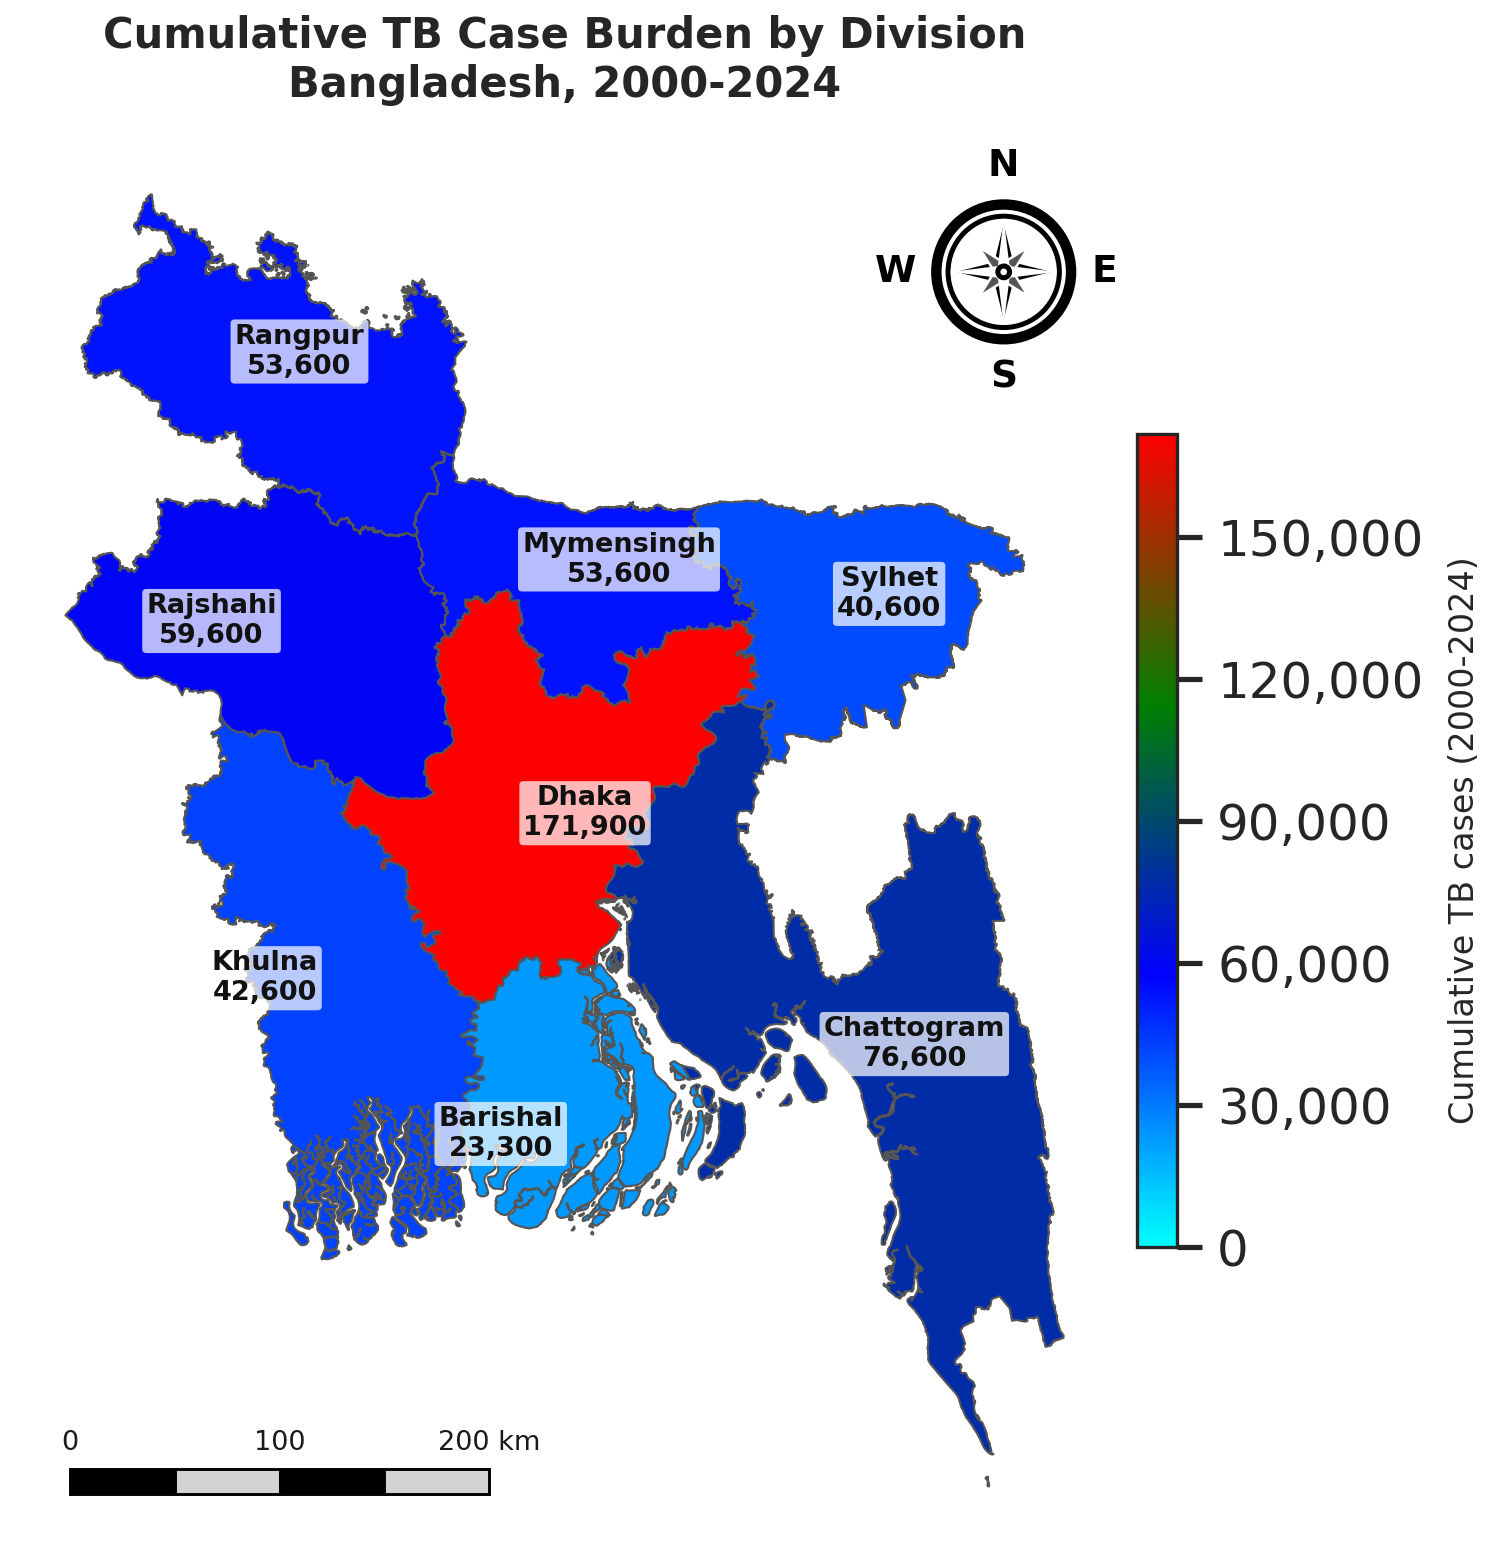
\includegraphics[width=\textwidth]{map1_cumulative_cases}
    \subcaption{Cumulative TB cases by division, 2000--2024.
      Darker shading indicates higher absolute case burden.}
    \label{fig:7a}
  \end{subfigure}
  \hfill
  \begin{subfigure}[t]{0.48\textwidth}
    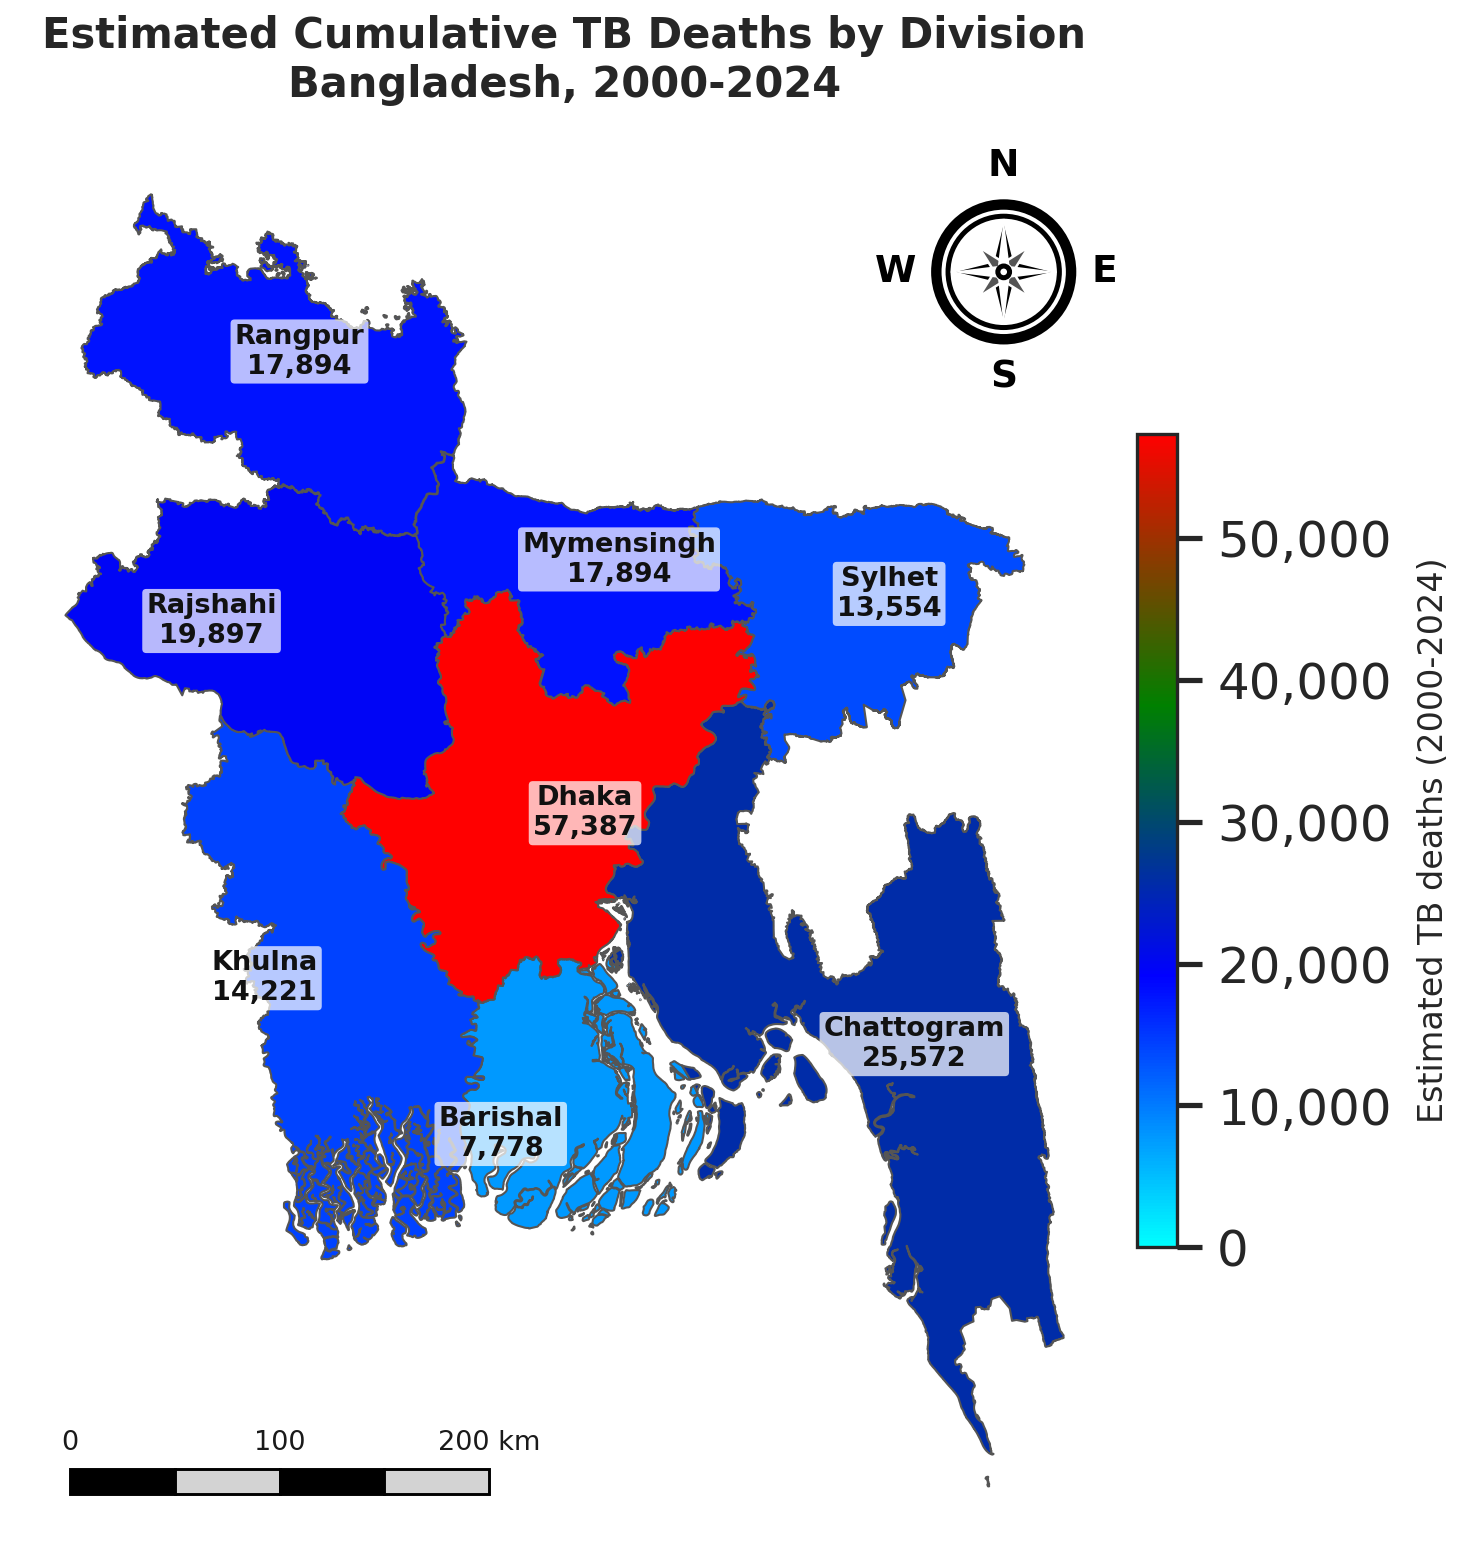
\includegraphics[width=\textwidth]{map2_cumulative_deaths}
    \subcaption{Estimated cumulative TB deaths by division, 2000--2024.
      Deaths estimated by applying the national case-fatality ratio to division case counts.}
    \label{fig:7b}
  \end{subfigure}
  \caption{\textbf{Cumulative geographic TB burden --- Bangladesh, 2000--2024.}
    The spatial concentration of cumulative cases and deaths mirrors population density:
    Dhaka and Chattogram divisions together bear $\sim$43\,\% of the 25-year case total
    and an equivalent share of estimated mortality.
    Barishal records the lowest burden in both panels, consistent with its
    lower population density and historically better TB indicators.
    \textit{Source: NTP Bangladesh / DGHS Annual Reports.}}
  \label{fig:geo_cumul}
\end{figure}
\clearpage

%% Figure 8 ─────────────────────────────────────────────────────────────────
\begin{figure}[htbp]
  \centering
  \begin{subfigure}[t]{\textwidth}
    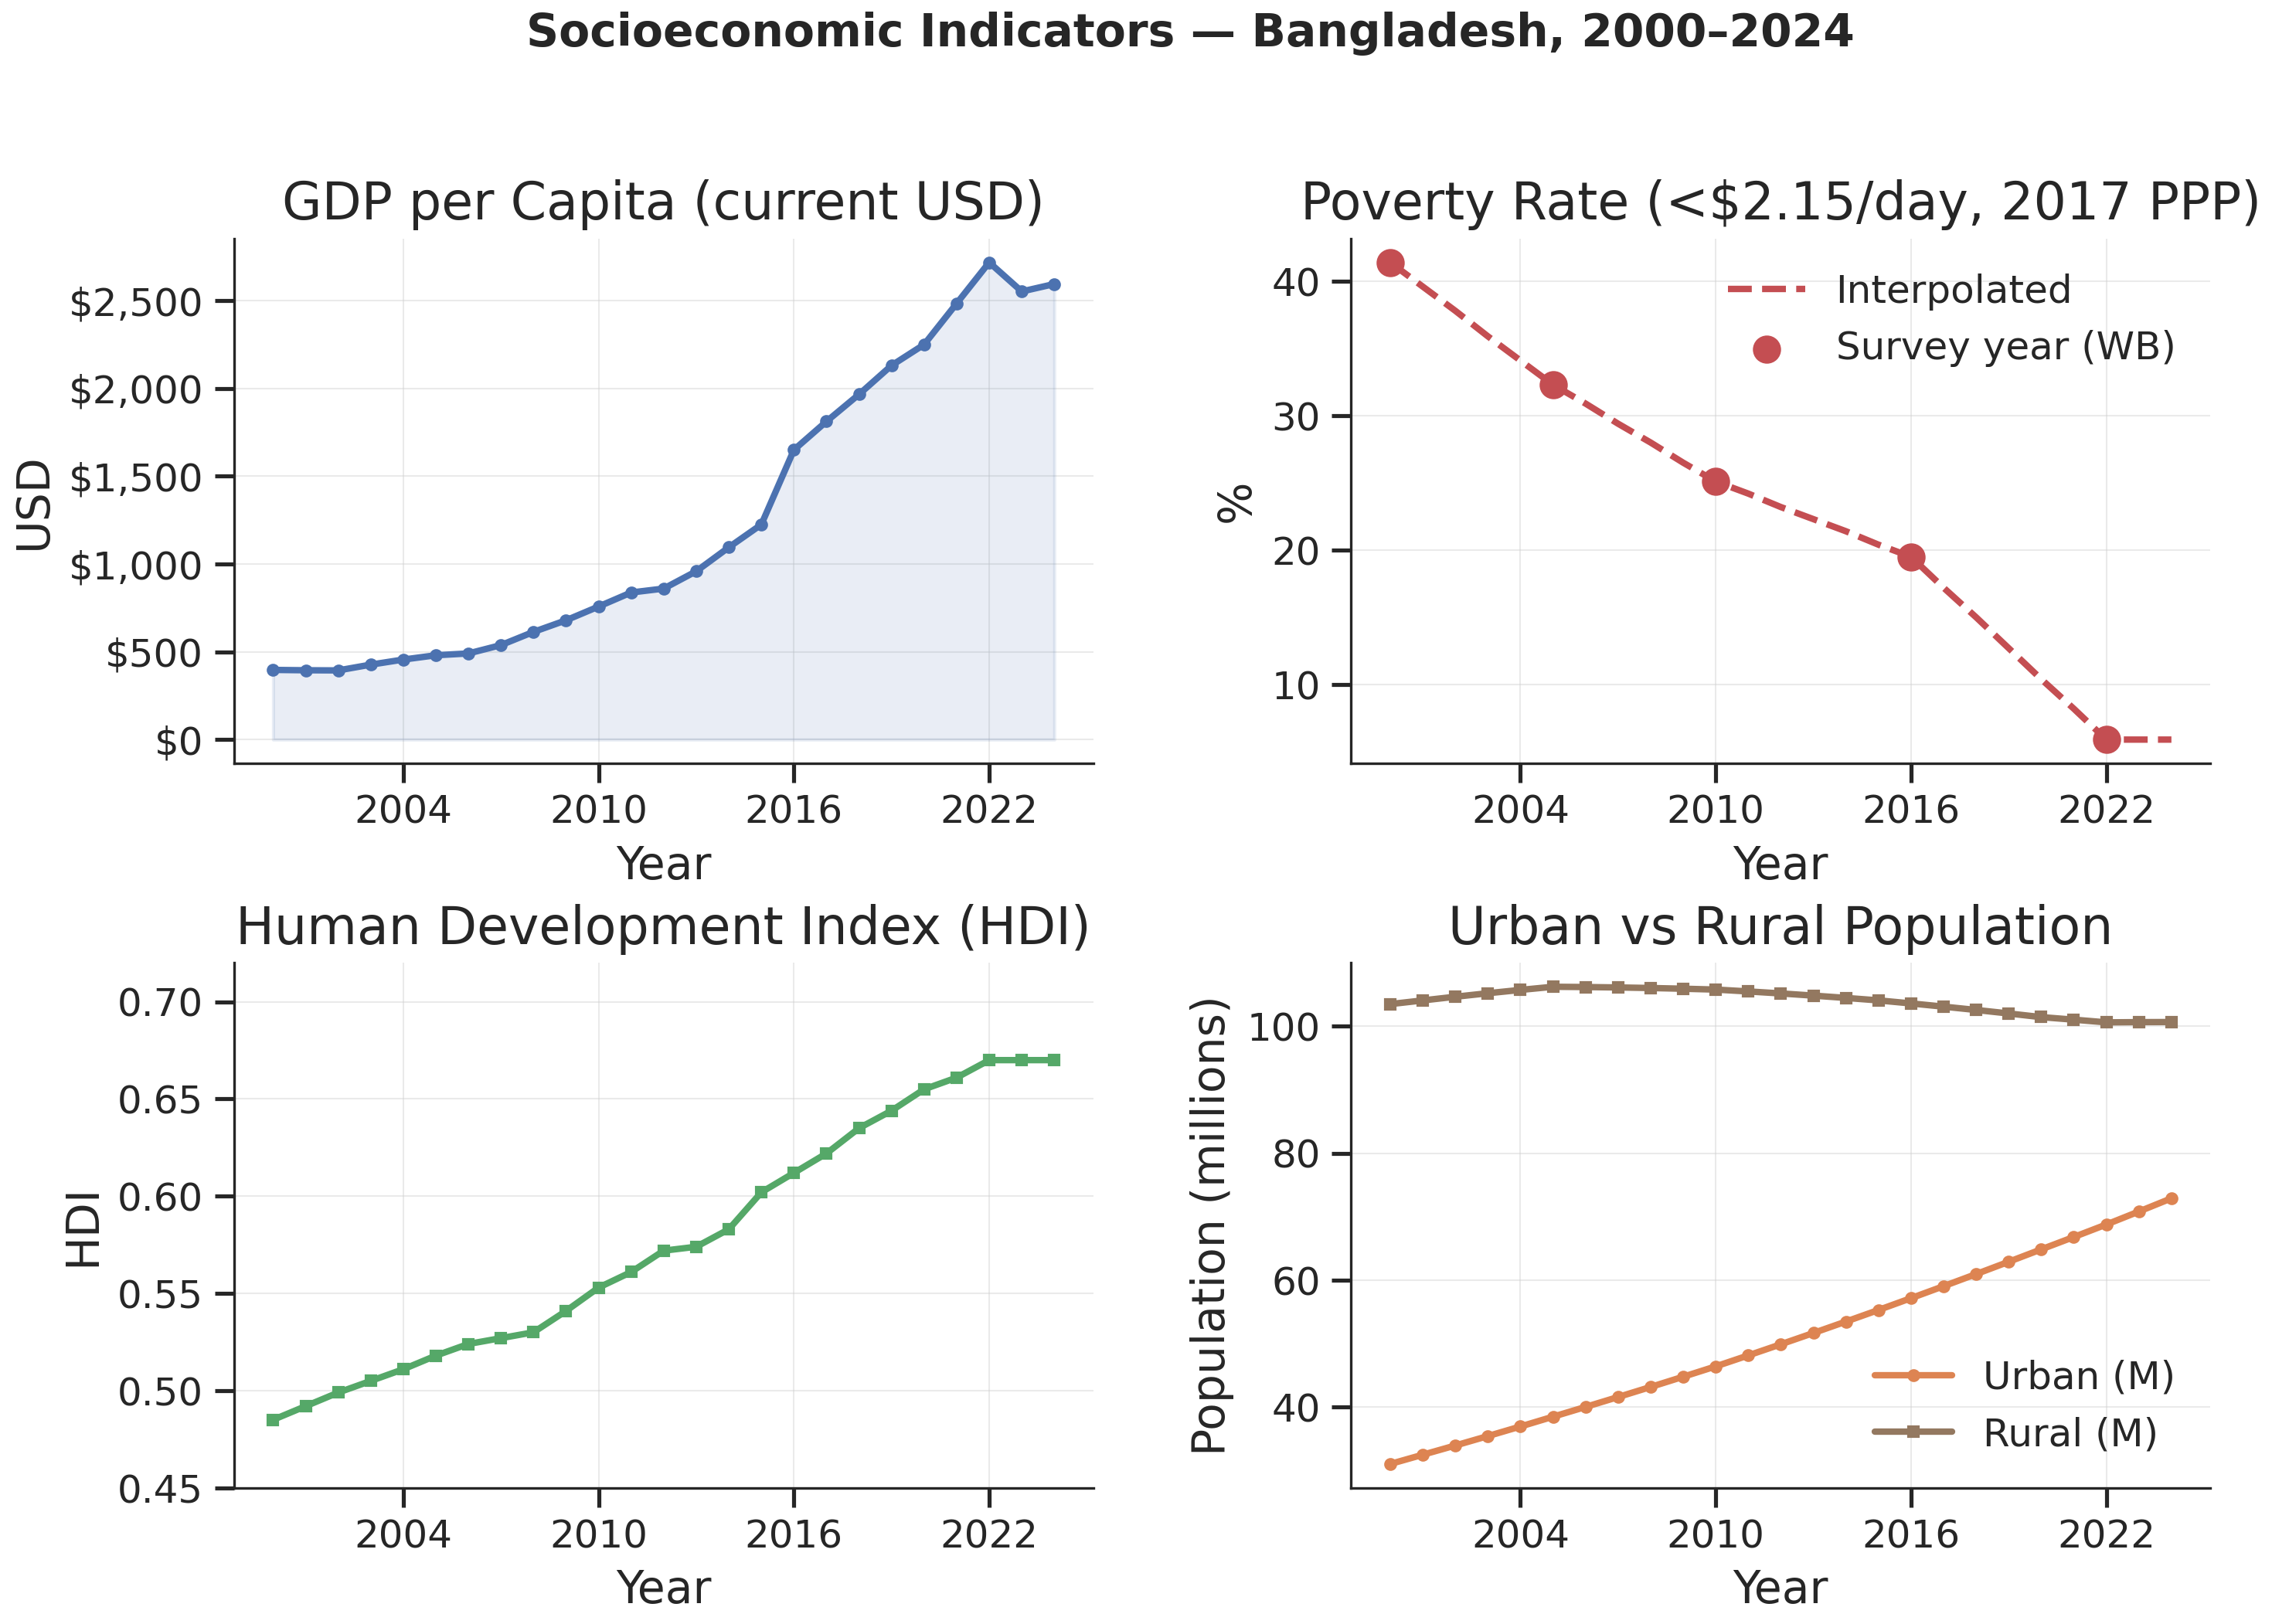
\includegraphics[width=\textwidth, height=0.38\textheight, keepaspectratio]{fig10_socioeconomic_trends}
    \subcaption{Socioeconomic indicator trends, 2000--2024.
      GDP per capita rose $\sim$5$\times$ in constant USD;
      poverty (below \$2.15/day) fell from 41\,\% to $<$6\,\%;
      the Human Development Index climbed from 0.47 to 0.68;
      and urban population grew from $\sim$25\,\% to $\sim$40\,\% of total.}
    \label{fig:8a}
  \end{subfigure}
  \vspace{0.8em}
  \begin{subfigure}[t]{0.60\textwidth}
    \centering
    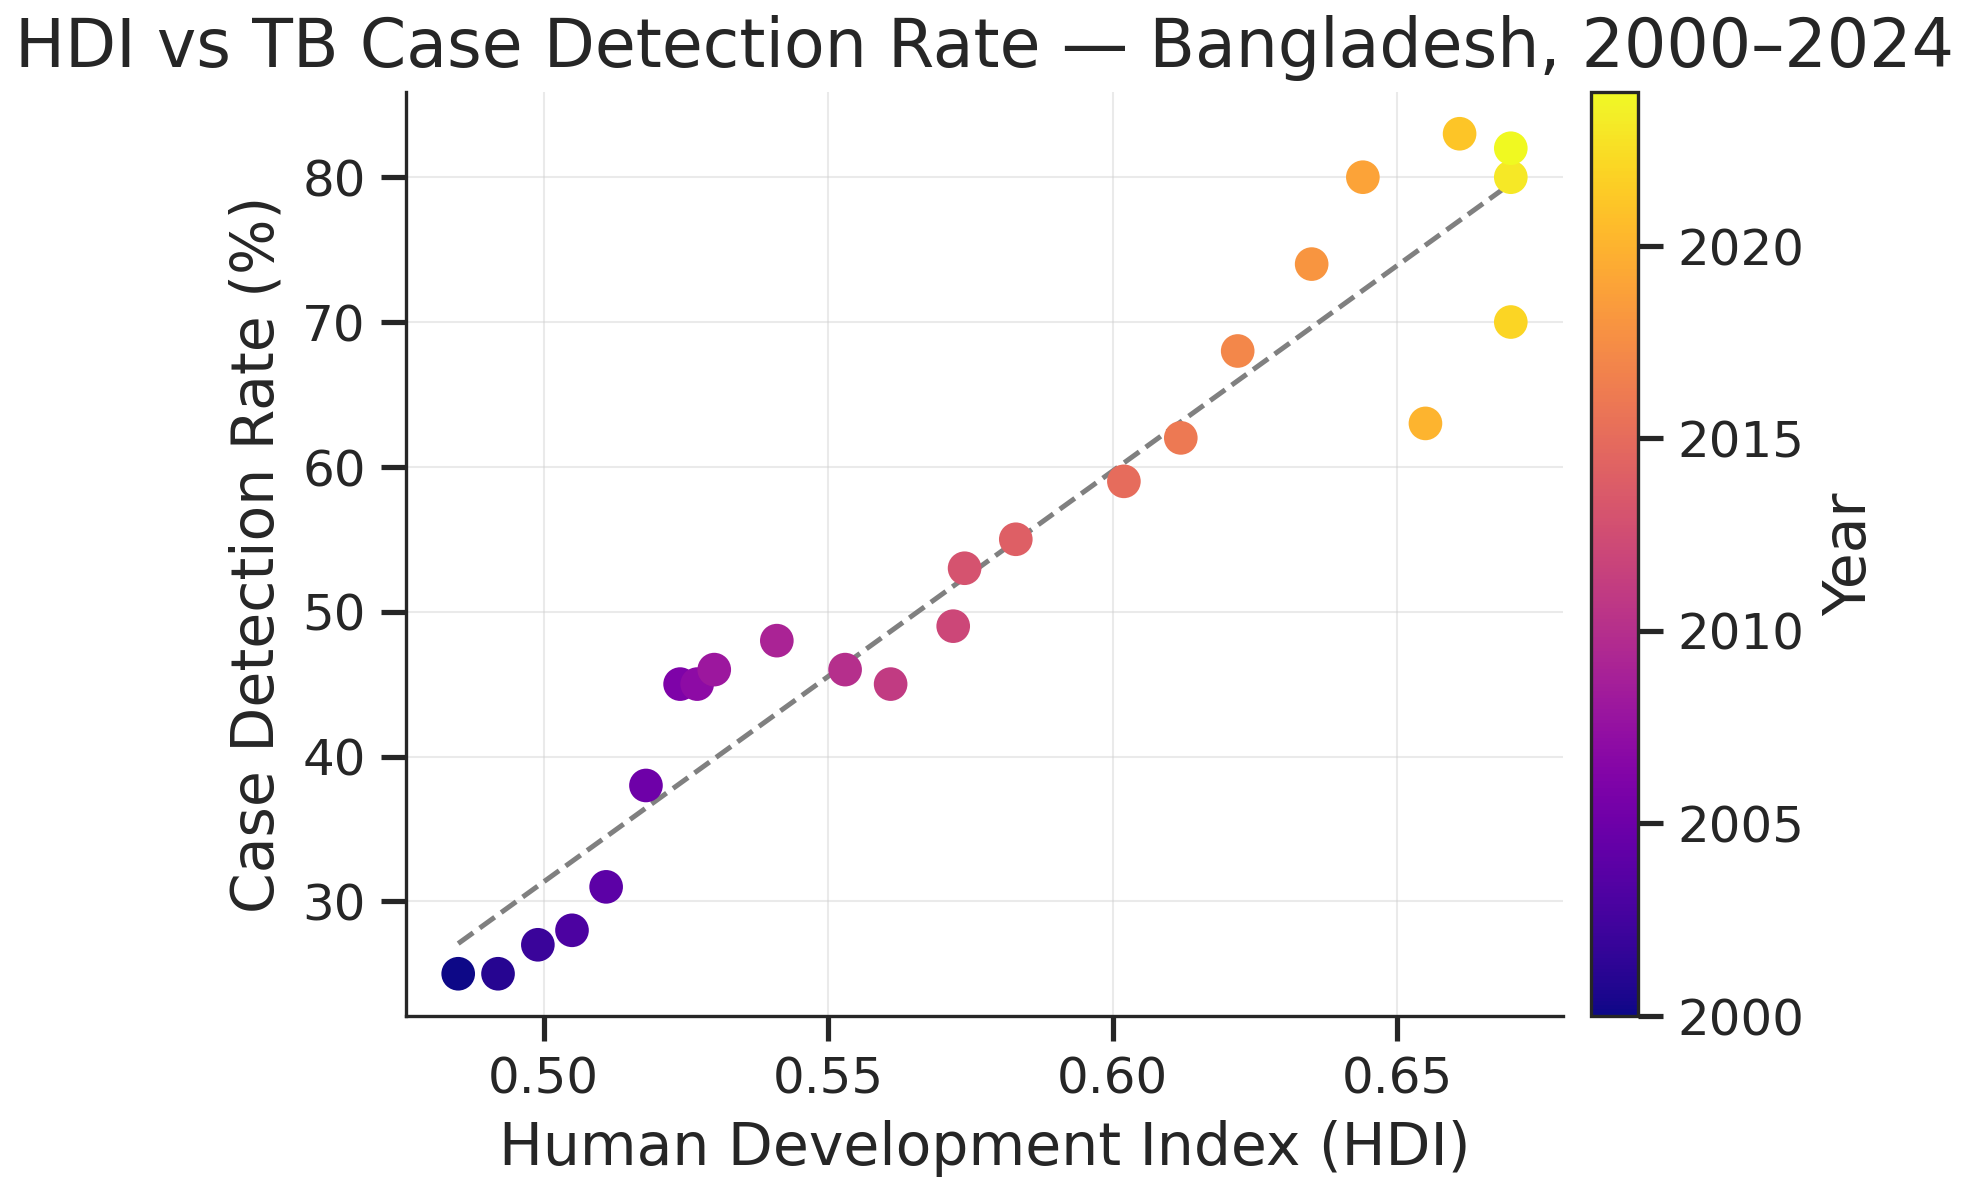
\includegraphics[width=\textwidth, height=0.32\textheight, keepaspectratio]{fig8_hdi_vs_cdr}
    \subcaption{HDI vs.\ Case Detection Rate --- each point is one year,
      colour-coded by calendar year.  The strong positive correlation
      ($r \approx +0.97$) confirms that human development gains
      are a structural enabler of improved TB case-finding.}
    \label{fig:8b}
  \end{subfigure}
  \caption{\textbf{Socioeconomic determinants of TB --- Bangladesh, 2000--2024.}
    Panel~(A) documents Bangladesh's remarkable development trajectory over the study period.
    Panel~(B) demonstrates that this trajectory closely tracks the country's
    capacity to detect TB cases: as the HDI rose, CDR rose in near-lockstep,
    suggesting that investments in education, health infrastructure and income
    simultaneously strengthened the TB response.
    \textit{Sources: World Bank Open Data (GDP, poverty, urbanisation);
    UNDP Human Development Reports; WHO Global TB Programme.}}
  \label{fig:socioeco}
\end{figure}
\clearpage

%% Figure 9 ─────────────────────────────────────────────────────────────────
\begin{figure}[htbp]
  \centering
  \begin{subfigure}[t]{0.54\textwidth}
    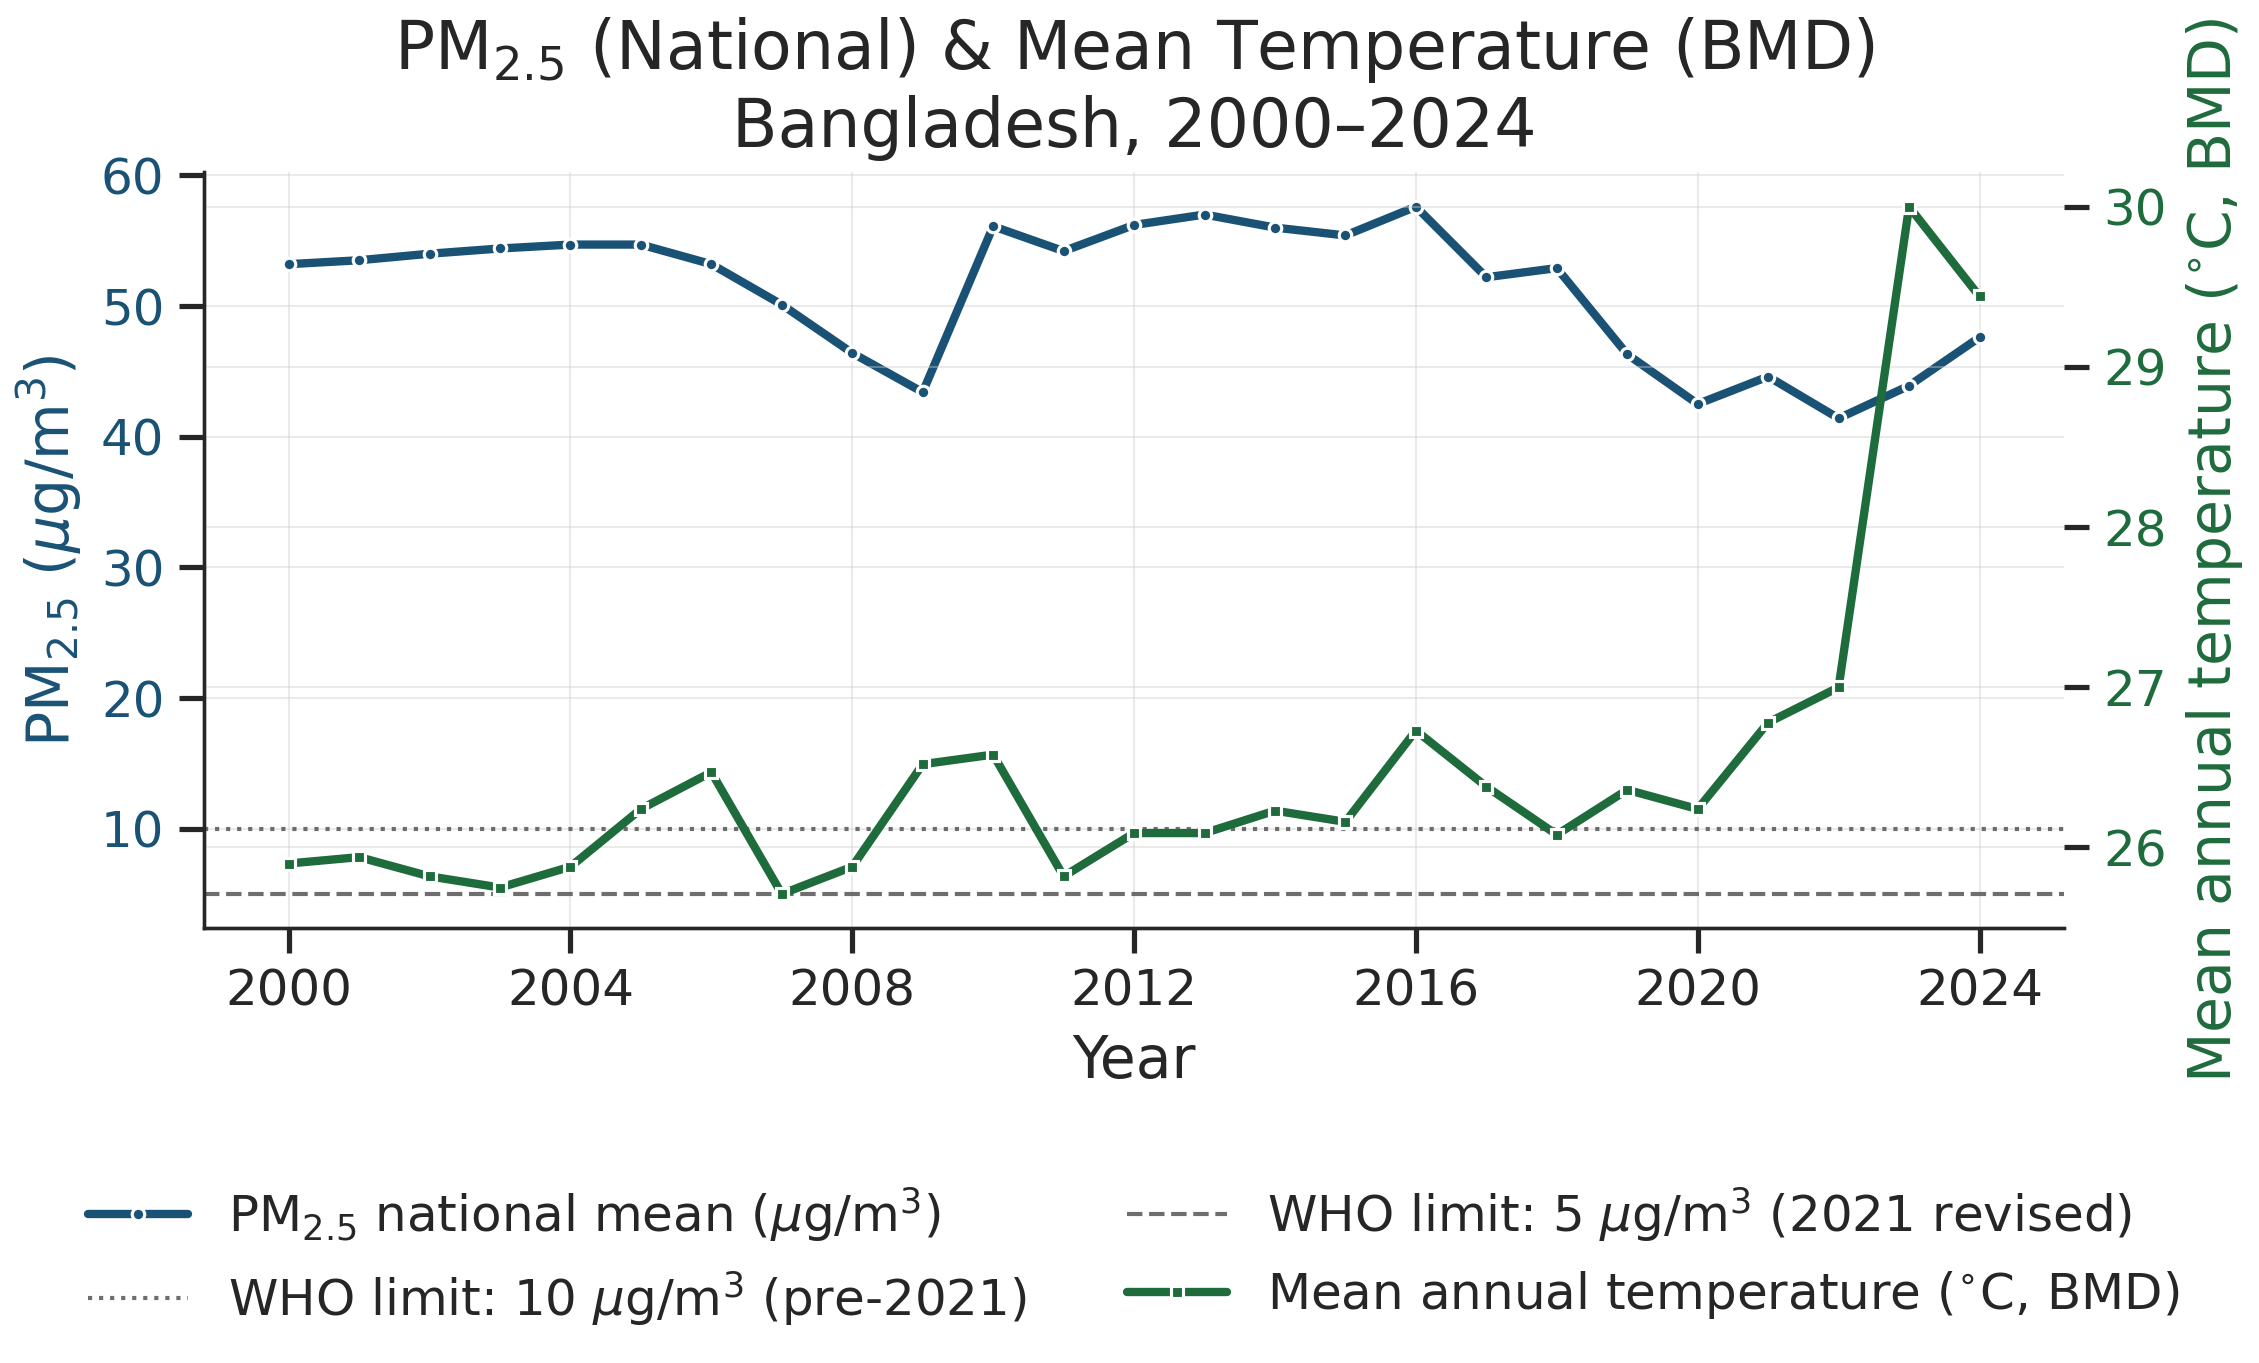
\includegraphics[width=\textwidth]{fig9_environmental}
    \subcaption{National mean PM\textsubscript{2.5} ($\mu$g\,m$^{-3}$, left axis)
      and mean annual temperature at the BMD Dhaka station (\textdegree C, right axis),
      2000--2024.
      Bangladesh consistently exceeds both the pre-2021 WHO guideline (10\,$\mu$g\,m$^{-3}$)
      and the 2021 revised guideline (5\,$\mu$g\,m$^{-3}$) by a factor of $5$--$10\times$,
      constituting a persistent environmental TB risk modifier.}
    \label{fig:9a}
  \end{subfigure}
  \hfill
  \begin{subfigure}[t]{0.44\textwidth}
    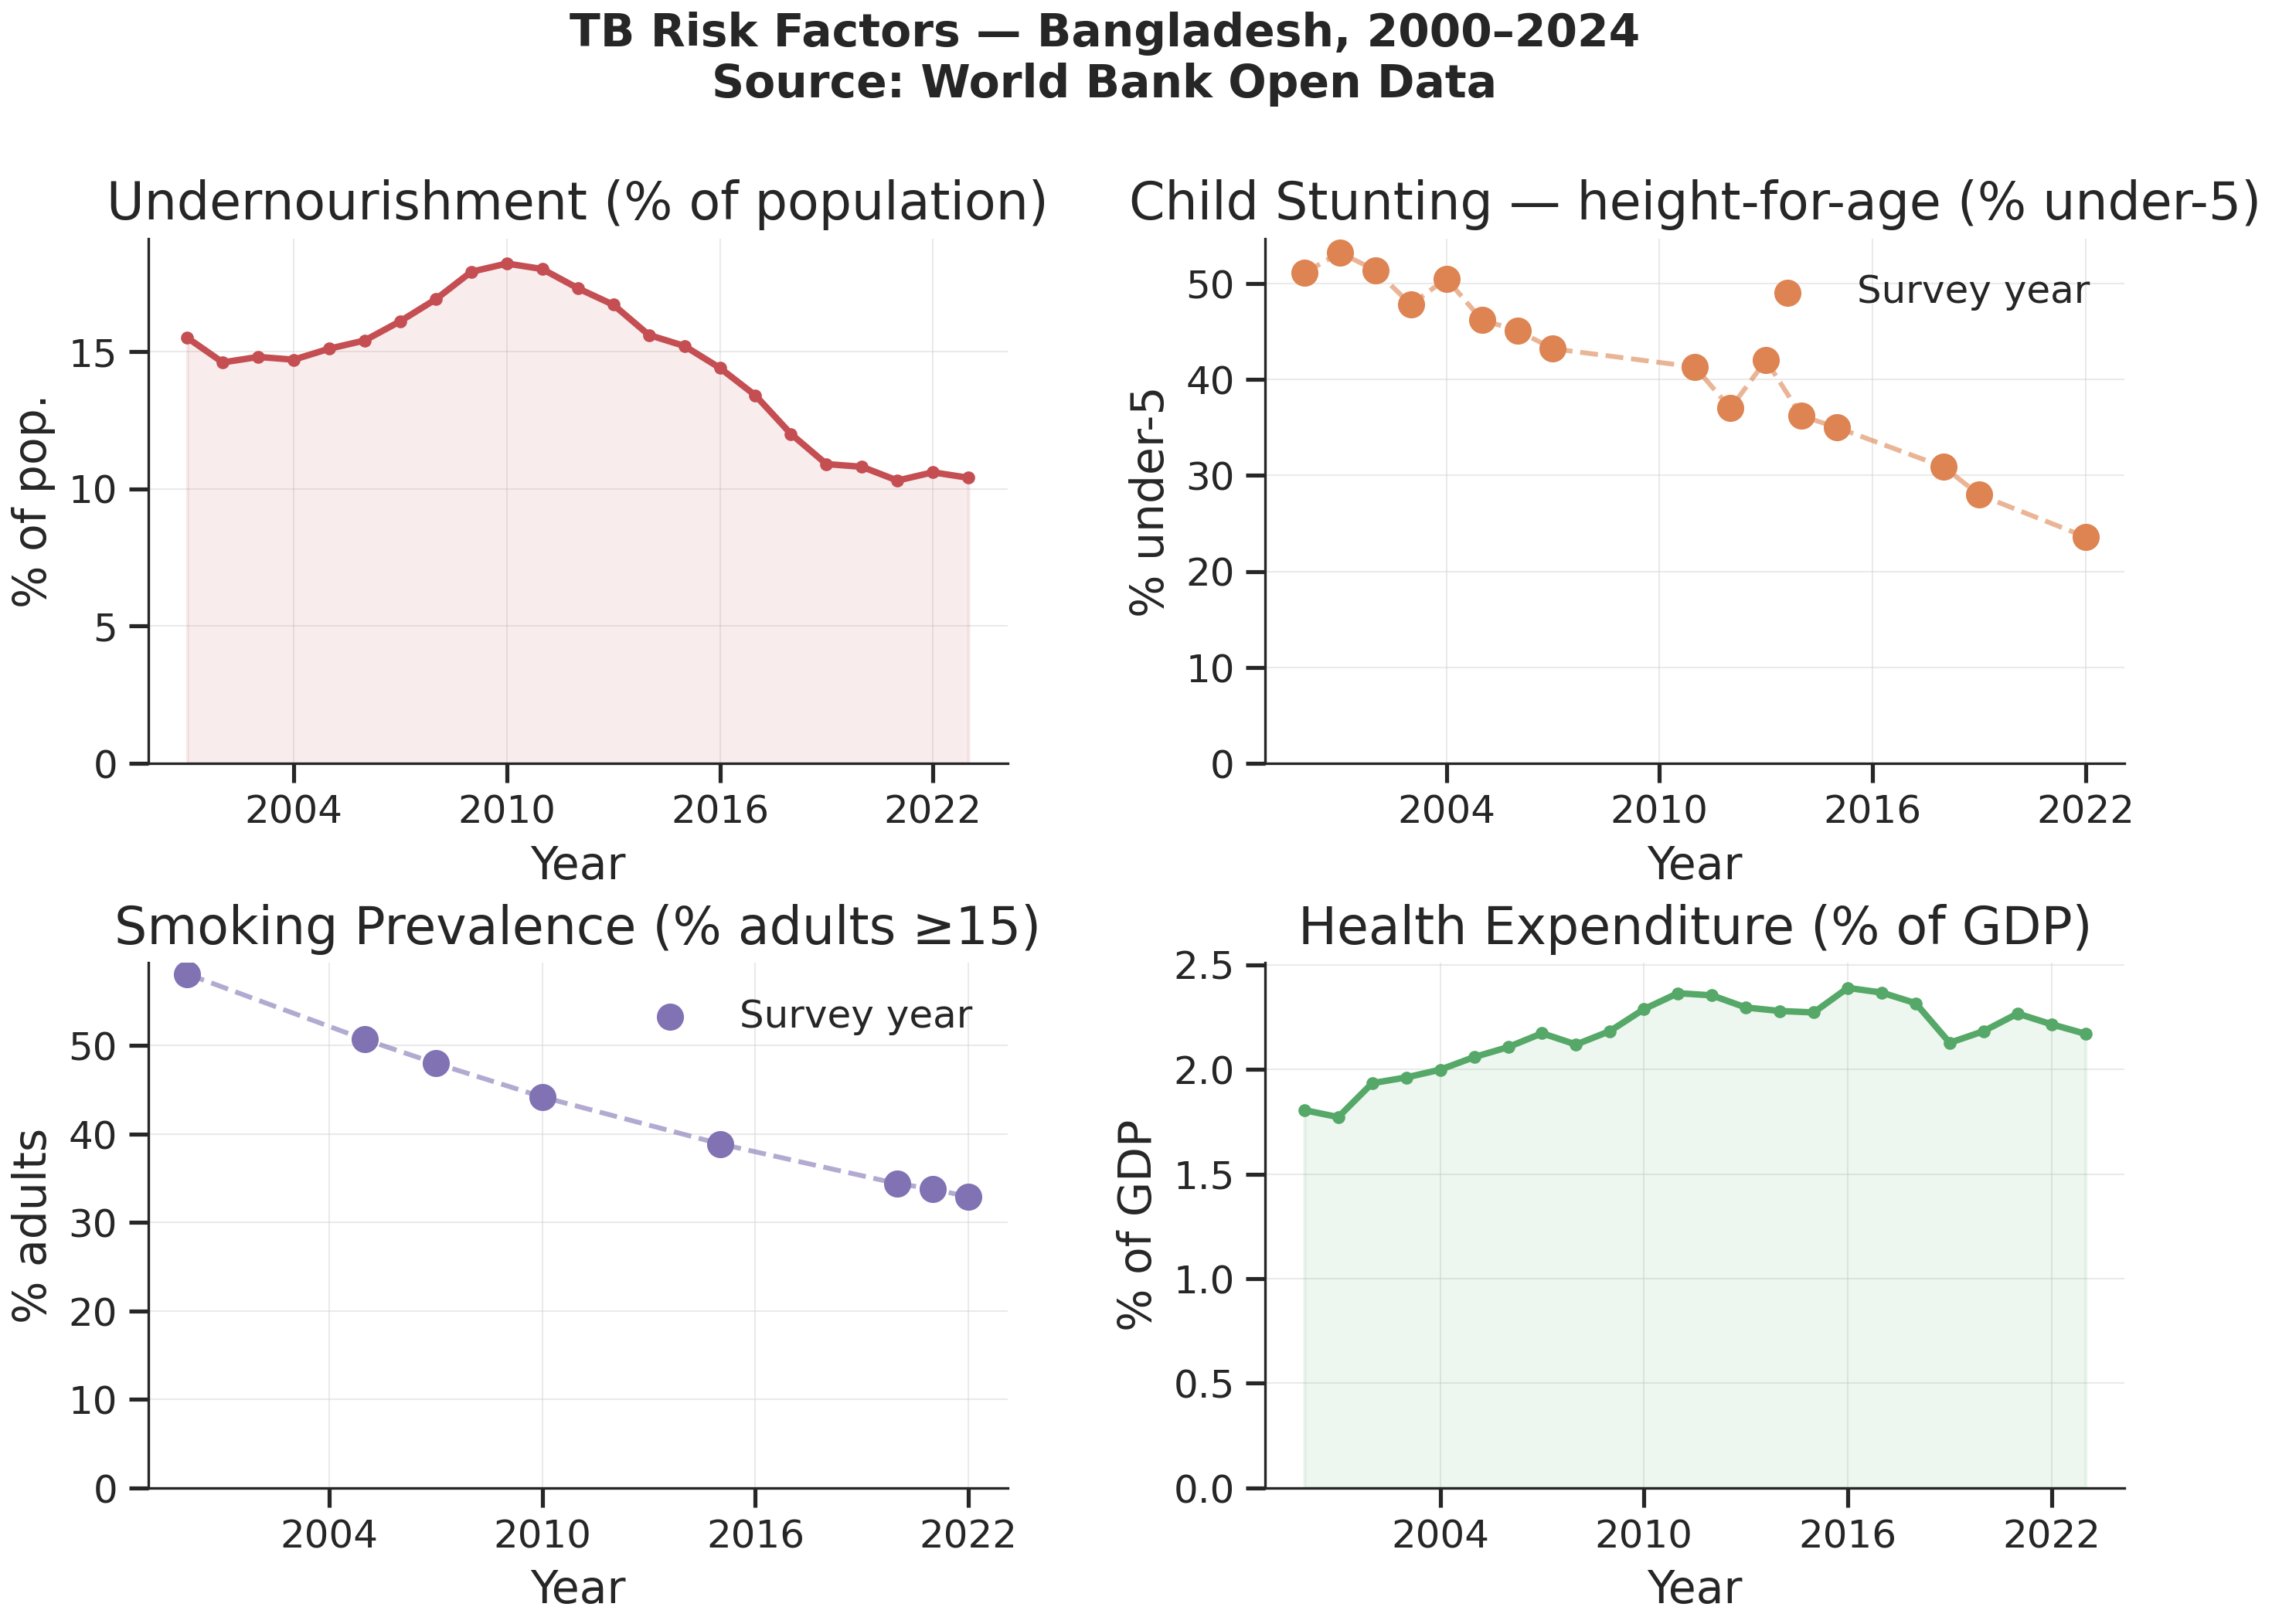
\includegraphics[width=\textwidth]{fig13_risk_factors}
    \subcaption{TB-associated behavioural and nutritional risk factor trends, 2000--2024.
      Undernourishment declined steadily; child stunting fell from $\sim$51\,\%
      to $\sim$24\,\% of under-fives; adult smoking prevalence decreased markedly;
      health expenditure as a share of GDP remained low but stable.}
    \label{fig:9b}
  \end{subfigure}
  \caption{\textbf{Environmental and behavioural risk factors for TB ---
    Bangladesh, 2000--2024.}
    Panel~(A) highlights air-pollution exposure as a structural environmental driver:
    PM\textsubscript{2.5} concentrations far exceed safe limits throughout the study period,
    impairing respiratory defences and amplifying susceptibility to airborne \textit{M.\ tuberculosis}.
    Panel~(B) shows that while nutritional and smoking risks have improved substantially,
    persistent undernutrition and a low health-expenditure share remain priority targets.
    \textit{Sources: World Bank (PM\textsubscript{2.5}, undernourishment, stunting, smoking,
    health expenditure); WHO GHO; CAMS/Open-Meteo; BMD.}}
  \label{fig:risk_factors}
\end{figure}
\clearpage

%% Figure 10 ─────────────────────────────────────────────────────────────────
\begin{figure}[htbp]
  \centering
  \begin{subfigure}[t]{0.44\textwidth}
    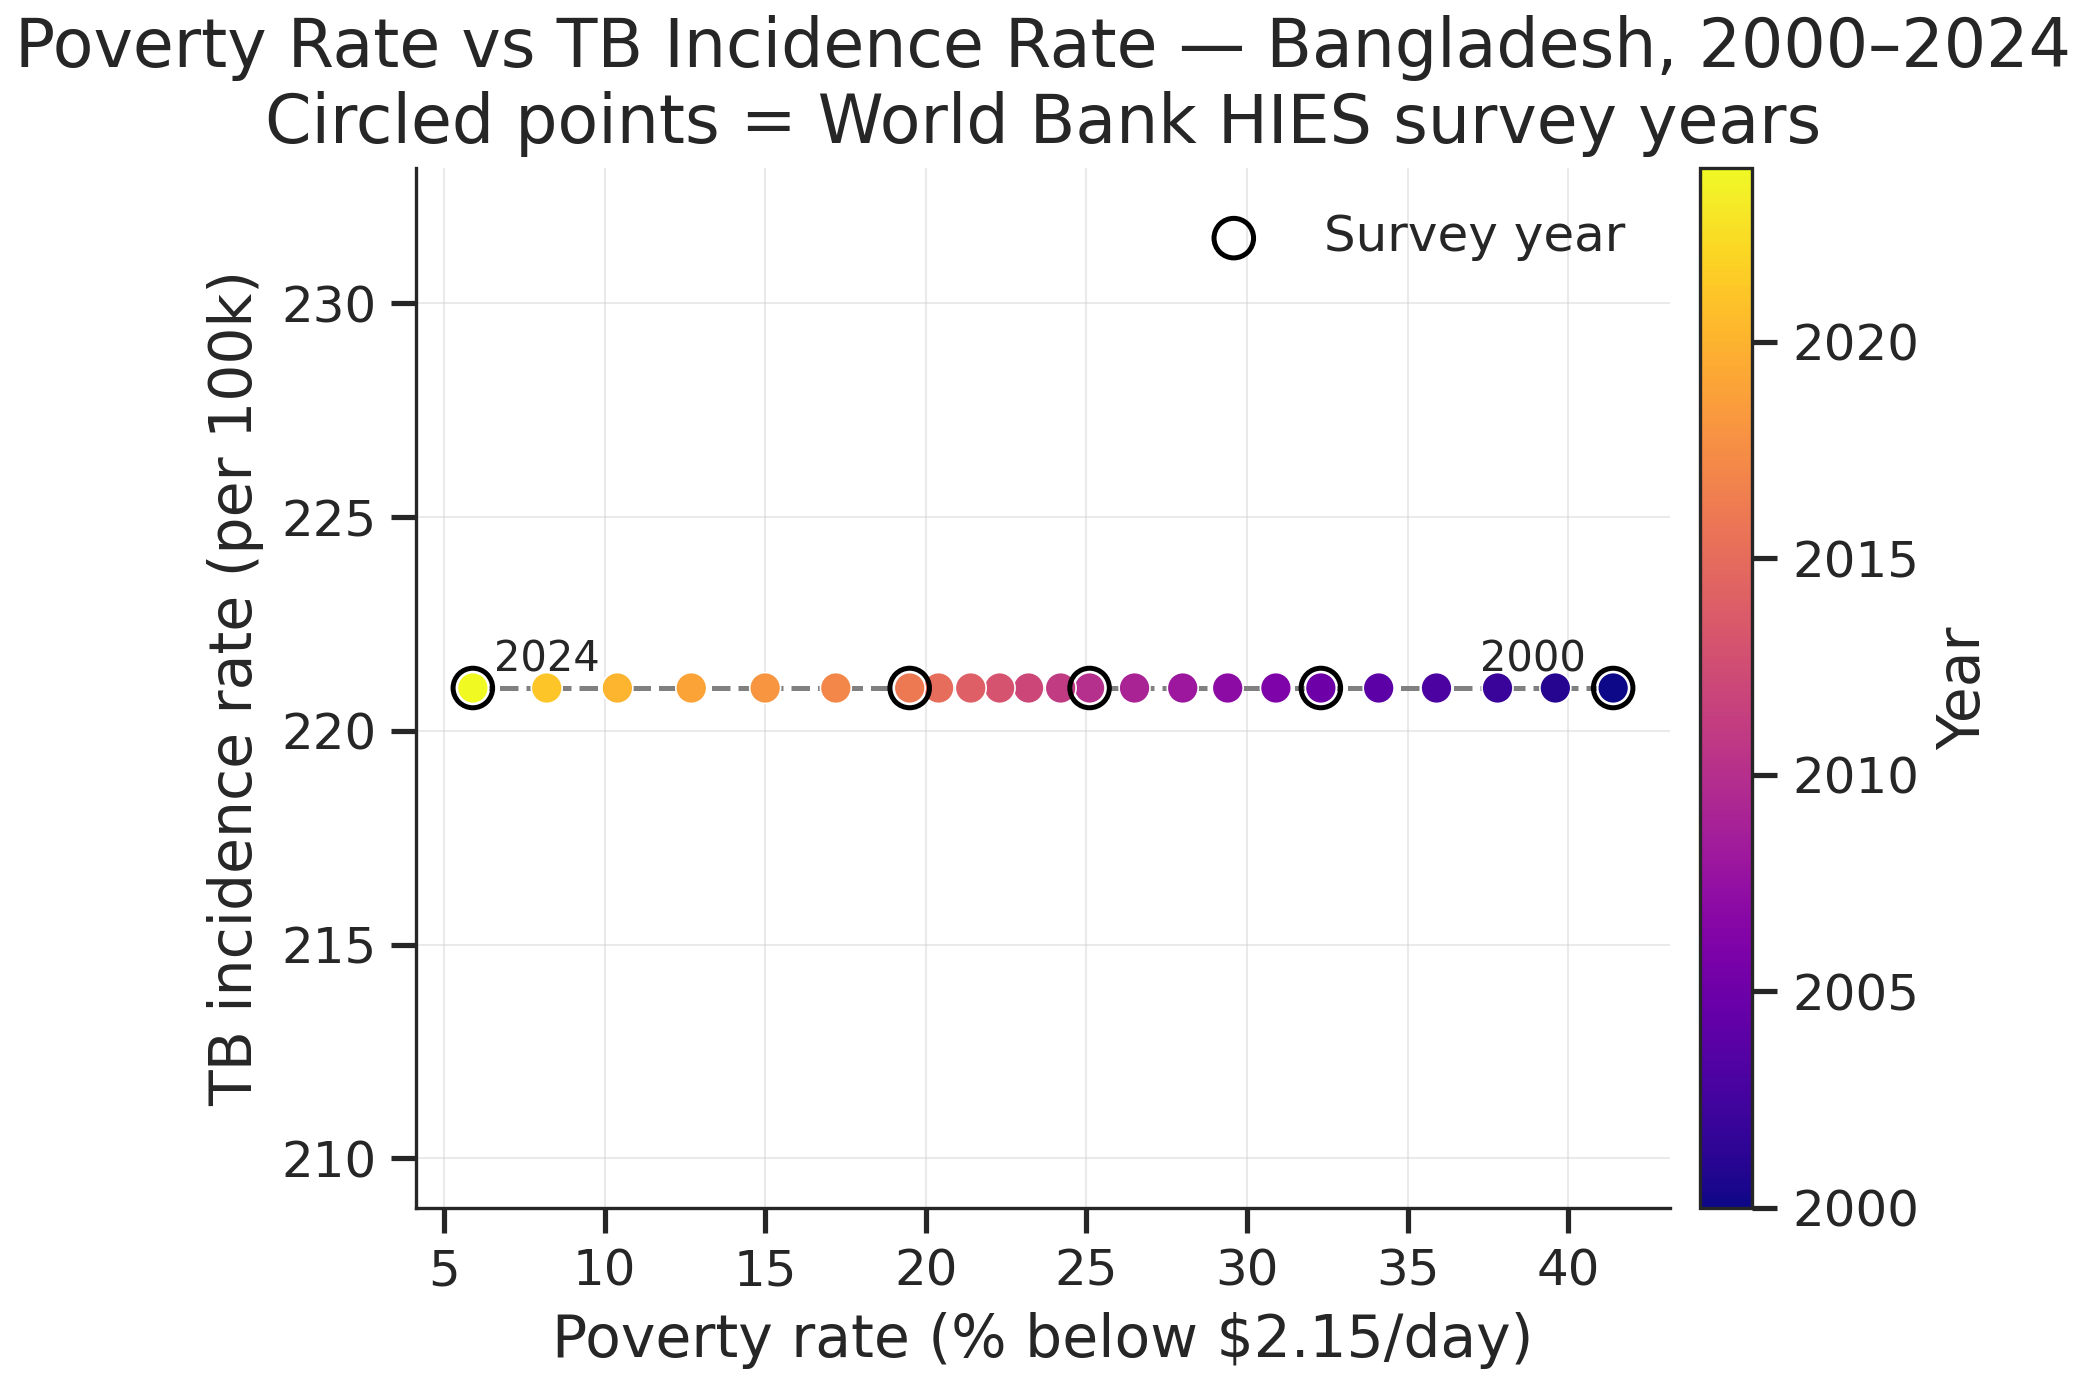
\includegraphics[width=\textwidth]{fig11_poverty_vs_tb}
    \subcaption{Poverty rate vs.\ TB incidence rate, 2000--2024.
      Each point is one year, colour-coded by calendar year;
      circled points are World Bank HIES survey years.
      The near-horizontal scatter reveals that TB incidence
      has remained remarkably flat ($\sim$220 per 100\,000) even as poverty
      fell from 41\,\% to $<$6\,\%, suggesting that detection improvements
      have kept notified incidence stable as the true burden declined.}
    \label{fig:10a}
  \end{subfigure}
  \hfill
  \begin{subfigure}[t]{0.54\textwidth}
    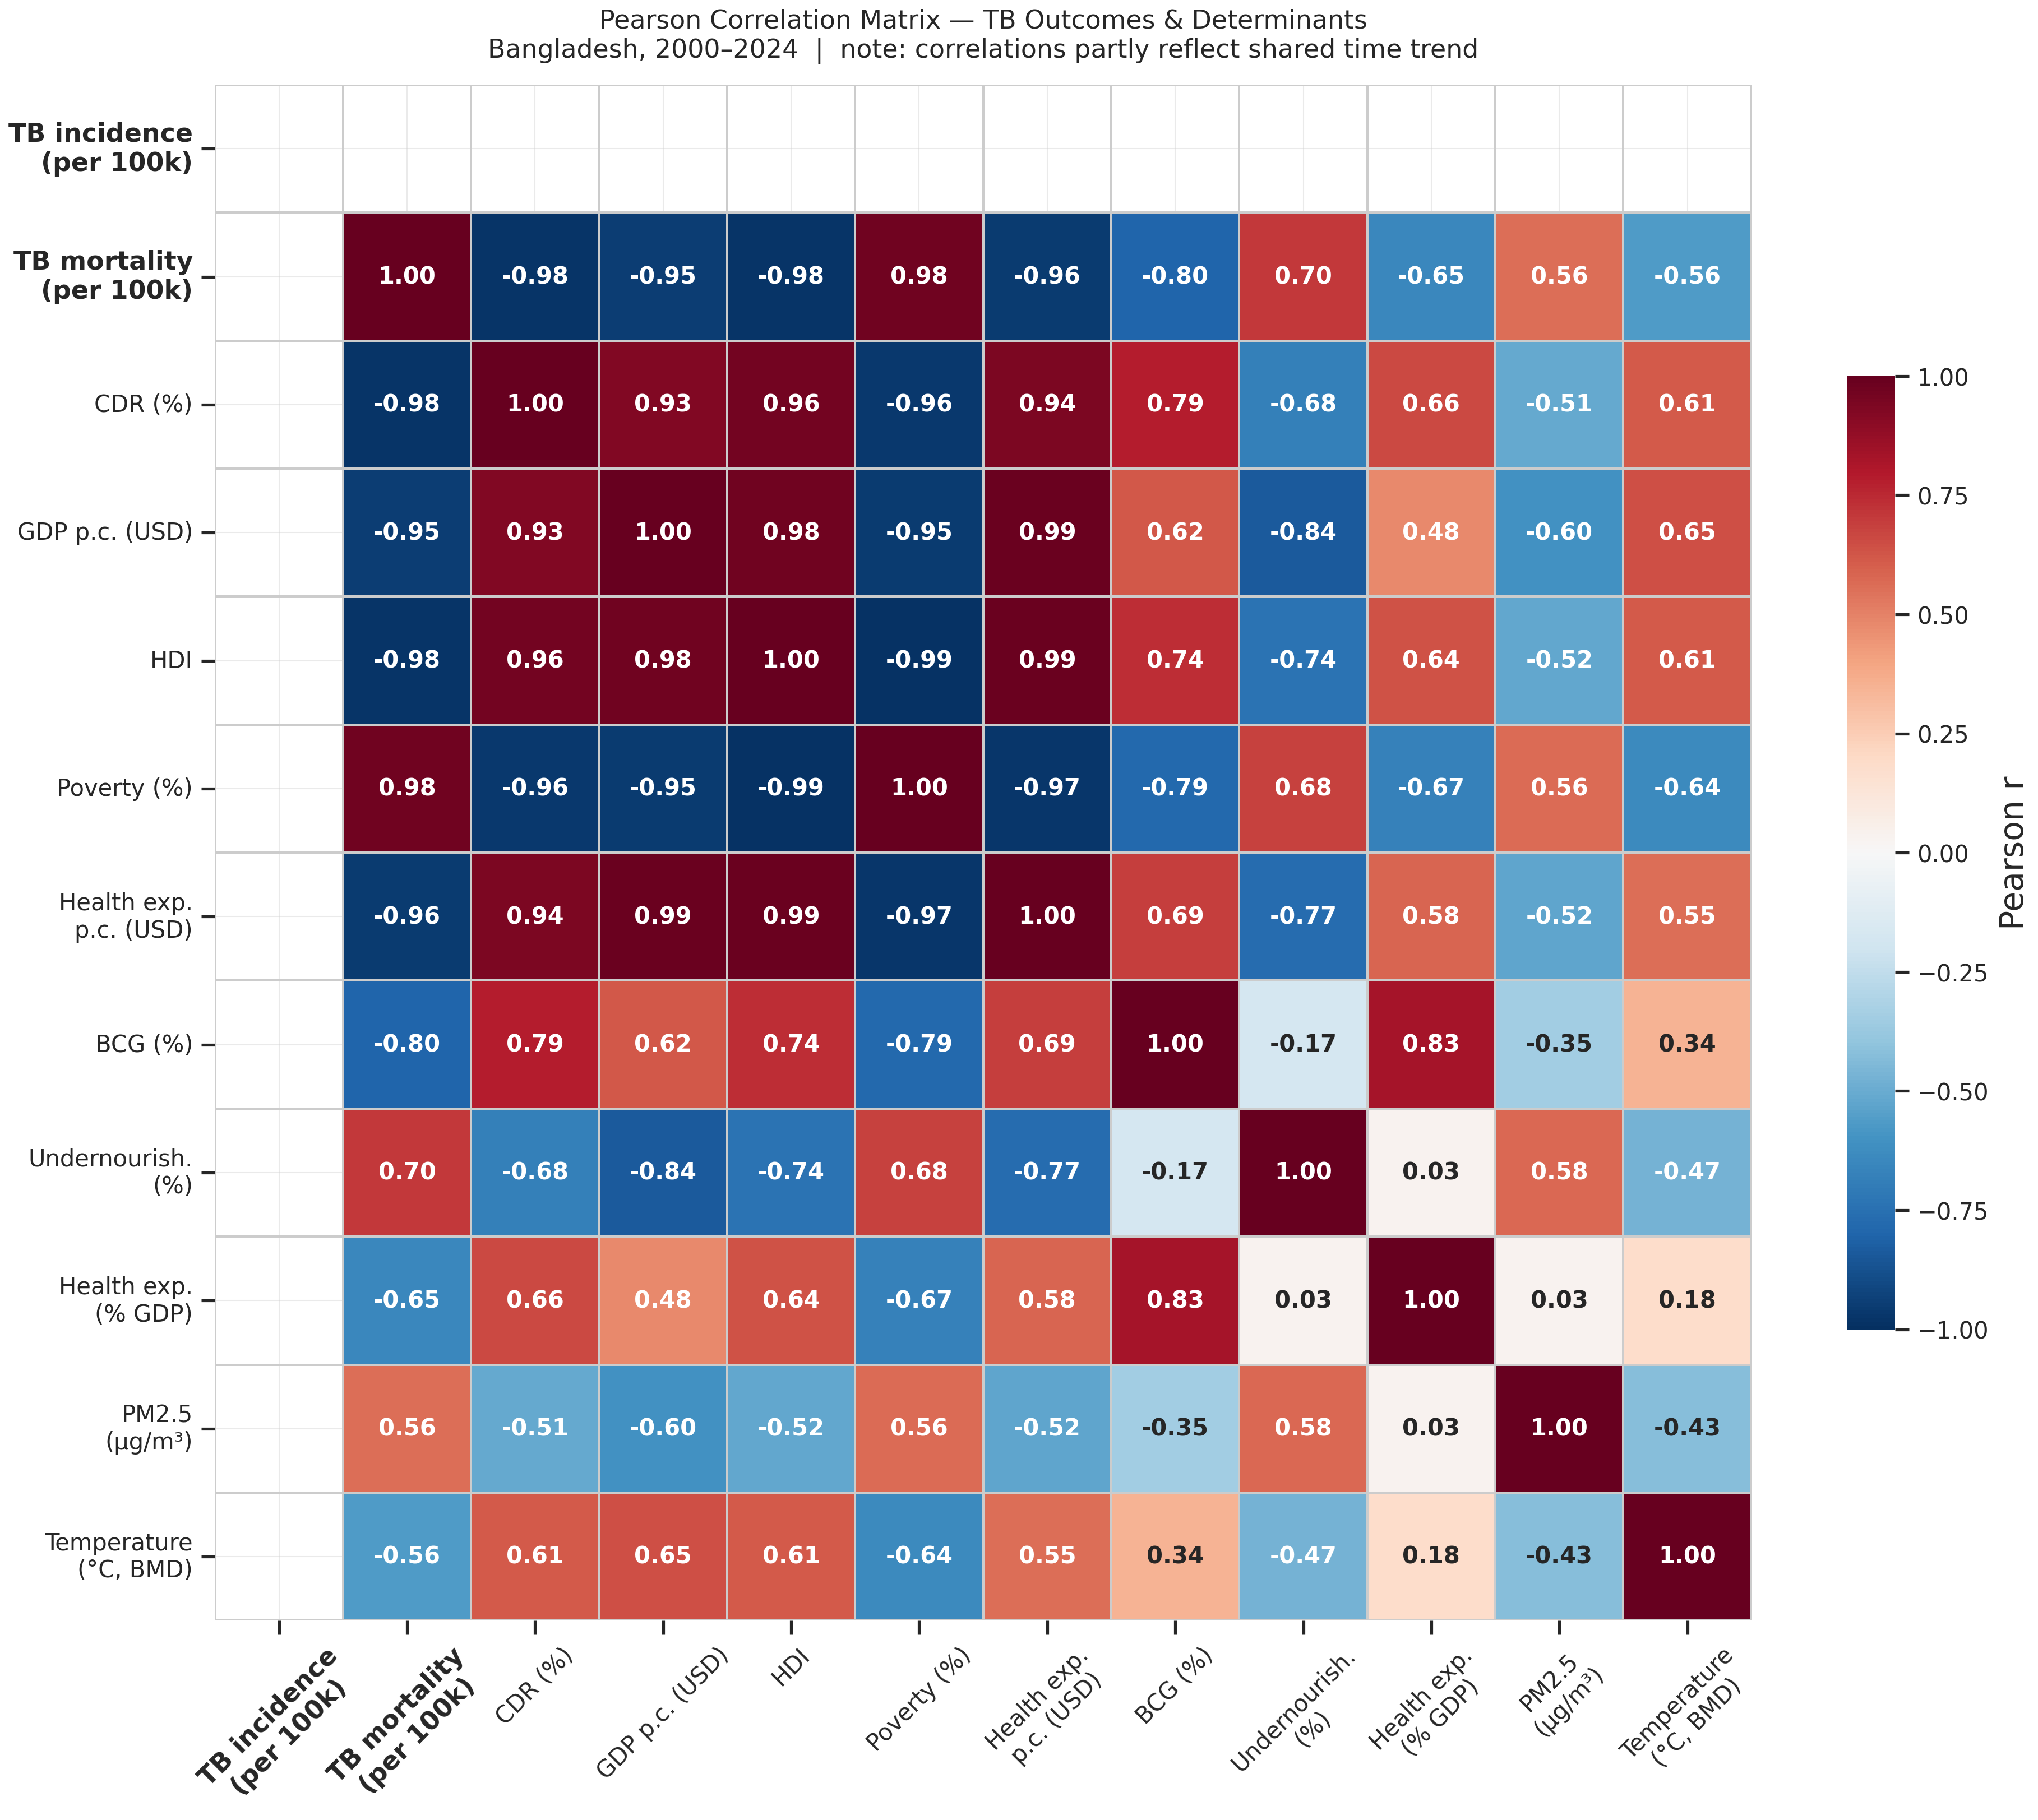
\includegraphics[width=\textwidth]{fig14_correlation_matrix}
    \subcaption{Pearson correlation matrix of TB outcomes and determinants.
      TB incidence and mortality (bold labels) show strong negative correlations
      with CDR, HDI, GDP and health expenditure ($r < -0.95$),
      and strong positive correlations with poverty ($r > +0.95$).
      Correlations partly reflect shared secular time trends;
      causal inference requires covariate adjustment.}
    \label{fig:10b}
  \end{subfigure}
  \caption{\textbf{Statistical associations between TB outcomes and key determinants ---
    Bangladesh, 2000--2024.}
    Panel~(A) illustrates the decoupling of poverty reduction from notified TB incidence,
    consistent with rising case detection masking a declining true burden.
    Panel~(B) provides a system-level view: virtually all socioeconomic and
    programme indicators correlate at $|r| > 0.9$ with TB outcomes,
    underscoring the multi-factorial nature of the epidemic and the importance
    of addressing poverty, nutrition, environment and health-system capacity simultaneously.
    \textit{Sources: WHO Global TB Programme; World Bank Open Data; UNDP; BMD.}}
  \label{fig:stats}
\end{figure}
\clearpage

%% Figure 11 ─────────────────────────────────────────────────────────────────
\begin{figure}[htbp]
  \centering
  \includegraphics[width=\textwidth]{fig15_pairplot}
  \caption{\textbf{Pairplot of TB outcomes against key determinants ---
    Bangladesh, 2000--2024.}
    Each of the 64 cells shows the bivariate relationship between one pair of
    the eight variables: TB incidence rate, TB mortality rate, GDP per capita,
    Human Development Index, poverty rate, undernourishment, BCG coverage,
    and PM\textsubscript{2.5} concentration.
    Points are colour-coded by time period:
    2000--08 (blue), 2009--16 (green), 2017--24 (red).
    Diagonal cells show kernel density estimates for each variable;
    lower-triangle cells show scatter plots; upper-triangle cells show scatter overlays.
    TB incidence and mortality labels are \textbf{bold}.
    The clear period-based clustering confirms the structural shift in Bangladesh's
    TB epidemiology across three phases of the national response.
    \textit{Sources: WHO Global TB Programme; World Bank Open Data; UNDP; BMD.}}
  \label{fig:pairplot}
\end{figure}

\end{document}
